\batchmode
\documentclass{book}
\usepackage[a4paper,top=2.5cm,bottom=2.5cm,left=2.5cm,right=2.5cm]{geometry}
\usepackage{makeidx}
\usepackage{natbib}
\usepackage{graphicx}
\usepackage{multicol}
\usepackage{float}
\usepackage{listings}
\usepackage{color}
\usepackage{ifthen}
\usepackage[table]{xcolor}
\usepackage{textcomp}
\usepackage{alltt}
\usepackage[utf8]{inputenc}
\usepackage{mathptmx}
\usepackage[scaled=.90]{helvet}
\usepackage{courier}
\usepackage{sectsty}
\usepackage{amssymb}
\usepackage[titles]{tocloft}
\usepackage{doxygen}
\lstset{language=C++,inputencoding=utf8,basicstyle=\footnotesize,breaklines=true,breakatwhitespace=true,tabsize=8,numbers=left }
\makeindex
\setcounter{tocdepth}{3}
\renewcommand{\footrulewidth}{0.4pt}
\renewcommand{\familydefault}{\sfdefault}
\hfuzz=15pt
\setlength{\emergencystretch}{15pt}
\hbadness=750
\tolerance=750
\begin{document}
\begin{titlepage}
\vspace*{7cm}
\begin{center}
{\Large Out\-\_\-\-Of\-\_\-\-Core \\[1ex]\large v1.\-0 }\\
\vspace*{1cm}
{\large 制作者 Doxygen 1.8.1.2}\\
\vspace*{0.5cm}
{\small 2012年 八月 5日 星期日 16:53:56}\\
\end{center}
\end{titlepage}
\clearemptydoublepage
\pagenumbering{roman}
\tableofcontents
\clearemptydoublepage
\pagenumbering{arabic}
\chapter{Out Of Core Image Processing Liabary}
\label{index}\section{介绍}\label{index_intro_sec}
通常的图像处理是基于内存进行的,但在图像数据非常大导致无法将数据全部装入内存处理的时候,基于内存的处理方法就会失效。\par
 Out Of Core技术就是用来解决这个问题。当数据很大的时候,实际的数据存放在硬盘上,在需要获取或者处理数据的时候, 再动态的从磁盘中加载数据到内存进行处理。\par


主要实现了下面几个类:
\begin{DoxyItemize}
\item \doxyref{Blockwise\-Image}{p.}{class_blockwise_image} 可以容纳大型的数据数据储存,提供对图像处理的通用性接口,同时可以将图像数据写入到磁盘中以备后续处理。
\item \doxyref{Hierarchical\-Image}{p.}{class_hierarchical_image} 继承自\-Blockwise\-Image,提供一致的图像处理接口,但在保存到磁盘时,将提取不同的层级的图像数据并写入磁盘,这样方便以后提取 不同分辨率下的图像数据。
\item \doxyref{Disk\-Big\-Image}{p.}{class_disk_big_image} 用来对由\-Blockwise\-Image和\-Hierarchical\-Image写入到磁盘中的图像数据进行动态的读写操作。
\end{DoxyItemize}

几个工程文件说明:
\begin{DoxyItemize}
\item Reading\-Big\-Image 图像浏览器的初步实现。
\item Test 对\-Blockwise\-Image的图像处理接口和\-Disk\-Big\-Image的读写接口进行了测试,还有一部分是关于不同索引方法的测试。
\item Write\-Block\-Wise\-Image 使用\-Blockwise\-Image写入图像数据
\item Write\-Hierarchical\-Image 使用\-Hierarchical\-Image写入图像数据
\item Time\-Consume\-Test 对\-Disk\-Big\-Image类的get\-\_\-pixels\-\_\-by\-\_\-level\-\_\-fast和get\-\_\-pixels\-\_\-by\-\_\-level速度上进行的测试。 \par

\end{DoxyItemize}\section{安装}\label{index_setup_sec}
\subsection{相关库}\label{index_libary_sec}

\begin{DoxyPre}
 {\bfseries 1. boost}
 使用到了boost的下面相关子库:
 data\_time iostreams filesystem system thread
 需要编译好上面的静态库\end{DoxyPre}



\begin{DoxyPre} {\bfseries 2. stxxl}
 是一个提供了基于stl的容器接口,同时将容器数据存放在硬盘中的库。
 Website : {\tt http://stxxl.sourceforge.net/} 
 安装说明:
 (1)将/SharedLibrary/stxxl/include 设置为头文件包含的地址
 (2)将/SharedLibrary/stxxl/lib 设置为lib包含的地址 
 (3)在工程文件中设置下面的command line (前提配置好了boost, 在链接 stxxl的库的时候, 会自动去链接boost的相关库)\end{DoxyPre}



\begin{DoxyPre} {\bfseries Debug :}
 C/C++ -- Command Line :
 -D\_FILE\_OFFSET\_BITS=64 -D\_LARGEFILE\_SOURCE -D\_LARGEFILE64\_SOURCE -D\_SECURE\_SCL=0 /Od /MDd /ZI -D\_RTLDLL -DBOOST\_LIB\_DIAGNOSTIC -DSTXXL\_BOOST\_TIMESTAMP -DSTXXL\_BOOST\_CONFIG -DSTXXL\_BOOST\_FILESYSTEM -DSTXXL\_BOOST\_THREADS -DSTXXL\_BOOST\_RANDOM /EHsc /EHs /wd4820 /wd4217 /wd4668 /wd4619 /wd4625 /wd4626 /wd4355 /wd4996 -D\_SCL\_SECURE\_NO\_DEPRECATE /F 16777216 /nologo /DSTXXL\_LIBNAME="stxxl\_debug"\end{DoxyPre}



\begin{DoxyPre} Linker -- Command Line :
 /STACK:16777216 /NOLOGO /DEBUG\end{DoxyPre}



\begin{DoxyPre} {\bfseries Release :}
 C/C++ -- Command Line :
 -D\_FILE\_OFFSET\_BITS=64 -D\_LARGEFILE\_SOURCE -D\_LARGEFILE64\_SOURCE -D\_SECURE\_SCL=0 /O2 /Ob2 /MD /DNDEBUG -D\_RTLDLL -DBOOST\_LIB\_DIAGNOSTIC -DSTXXL\_BOOST\_TIMESTAMP -DSTXXL\_BOOST\_CONFIG -DSTXXL\_BOOST\_FILESYSTEM -DSTXXL\_BOOST\_THREADS -DSTXXL\_BOOST\_RANDOM /EHsc /EHs /wd4820 /wd4217 /wd4668 /wd4619 /wd4625 /wd4626 /wd4355 /wd4996 -D\_SCL\_SECURE\_NO\_DEPRECATE /F 16777216 /nologo /DSTXXL\_LIBNAME="stxxl\_release"\end{DoxyPre}



\begin{DoxyPre} Linker -- Command Line :
 /STACK:16777216 /NOLOGO /OPT:REF\end{DoxyPre}



\begin{DoxyPre} (4)stxxl的配置文件,在代码运行的目录下面新建文件config.stxxl
 For example : #config.stxxl
 disk=c:,70000,wincall     
 disk=d:,70000,wincall
 disk=e:,70000,wincall
 #表示在在c,d,e中分别建立70000M大小的文件stxxl用来保存数据用。
 #对于Out\_Of\_Core模块而言,大小取决于图像的数据大小,比如一个102400*102400的图像而言,
 如果图像是RGB个格式,那么总大小为30G的图像。由于使用了zorder进行存储,存在数据冗余。
 使用zorder作为索引格式的话,最多是为原来大小的4倍,一般为2倍左右,所以分配60G到120G比较合适。\end{DoxyPre}



\begin{DoxyPre} {\bfseries 3. OpenCV}
 如果定义了宏 SAVE\_MINI\_IMAGE
 在将图像写入到磁盘中的时候,同时也会产生一张由用户指定分辨率大小的jpg格式图像文件,该文件是图像的缩略图用来方便得到显示效果
 将使用到了OpenCV的下面模块
 core highgui imgproc
 \end{DoxyPre}
 \begin{DoxyNote}{注解}
默认是没有定义\-S\-A\-V\-E\-\_\-\-M\-I\-N\-I\-\_\-\-I\-M\-A\-G\-E \par

\end{DoxyNote}
\section{Out Of Core模块代码}\label{index_src_sec}
所有代码都是模板类或者是放在.\-h文件中的inline函数,直接include到代码中编译即可。\par
 代码放在了/\-Platform/\-Out\-Of\-Core/include/ 文件夹下 
\chapter{类索引}
\section{类继承关系}
此继承关系列表按字典顺序粗略的排序\-: \begin{DoxyCompactList}
\item \contentsline{section}{Disk\-Big\-Image$<$ T $>$\-:\-:Data\-Index\-Info}{\pageref{struct_disk_big_image_1_1_data_index_info}}{}
\item \contentsline{section}{Disk\-Big\-Image\-Interface$<$ T $>$}{\pageref{class_disk_big_image_interface}}{}
\begin{DoxyCompactList}
\item \contentsline{section}{Disk\-Big\-Image$<$ T $>$}{\pageref{class_disk_big_image}}{}
\end{DoxyCompactList}
\item \contentsline{section}{Image\-File\-L\-R\-U$<$ T $>$}{\pageref{class_image_file_l_r_u}}{}
\item \contentsline{section}{Image\-Interface$<$ T $>$}{\pageref{class_image_interface}}{}
\begin{DoxyCompactList}
\item \contentsline{section}{Giant\-Image\-Interface$<$ T $>$}{\pageref{class_giant_image_interface}}{}
\begin{DoxyCompactList}
\item \contentsline{section}{Blockwise\-Image$<$ T, memory\-\_\-usage $>$}{\pageref{class_blockwise_image}}{}
\begin{DoxyCompactList}
\item \contentsline{section}{Hierarchical\-Image$<$ T, memory\-\_\-usage $>$}{\pageref{class_hierarchical_image}}{}
\end{DoxyCompactList}
\end{DoxyCompactList}
\end{DoxyCompactList}
\item \contentsline{section}{Index\-Method\-Interface}{\pageref{class_index_method_interface}}{}
\begin{DoxyCompactList}
\item \contentsline{section}{Block2\-D\-Index}{\pageref{class_block2_d_index}}{}
\item \contentsline{section}{Z\-Order\-Index}{\pageref{class_z_order_index}}{}
\item \contentsline{section}{Z\-Order\-Index\-Intuition}{\pageref{class_z_order_index_intuition}}{}
\end{DoxyCompactList}
\item \contentsline{section}{Pixel\-Element$<$ T $>$}{\pageref{struct_pixel_element}}{}
\item \contentsline{section}{Row\-Major\-Point}{\pageref{struct_row_major_point}}{}
\item \contentsline{section}{Size}{\pageref{struct_size}}{}
\end{DoxyCompactList}

\chapter{类索引}
\section{类列表}
这里列出了所有类、结构、联合以及接口定义等,并附带简要说明\-:\begin{DoxyCompactList}
\item\contentsline{section}{{\bf Block2\-D\-Index} }{\pageref{class_block2_d_index}}{}
\item\contentsline{section}{{\bf Blockwise\-Image$<$ T, memory\-\_\-usage $>$} \\*Derived from \doxyref{Giant\-Image\-Interface}{p.}{class_giant_image_interface}, support the big image operation, and saves the whole image into disk }{\pageref{class_blockwise_image}}{}
\item\contentsline{section}{{\bf Disk\-Big\-Image$<$ T $>$\-::\-Data\-Index\-Info} \\*This structure is used in the \doxyref{get\-\_\-pixels\-\_\-by\-\_\-level()}{p.}{class_disk_big_image_a9b8062ca60135249493571a6f47da1ef} function to sort the range data }{\pageref{struct_disk_big_image_1_1_data_index_info}}{}
\item\contentsline{section}{{\bf Disk\-Big\-Image$<$ T $>$} \\*Derived from \doxyref{Disk\-Big\-Image\-Interface}{p.}{class_disk_big_image_interface}, support for the reading and writing of the big image that was saved in the disk }{\pageref{class_disk_big_image}}{}
\item\contentsline{section}{{\bf Disk\-Big\-Image\-Interface$<$ T $>$} \\*The interface for accessing the big image files in the disk that were saved by \doxyref{Blockwise\-Image}{p.}{class_blockwise_image} and \doxyref{Hierarchical\-Image}{p.}{class_hierarchical_image} classes }{\pageref{class_disk_big_image_interface}}{}
\item\contentsline{section}{{\bf Giant\-Image\-Interface$<$ T $>$} \\*Derived form the \doxyref{Image\-Interface}{p.}{class_image_interface}, and defines the basic operations that restricted to the big image file accessing and operation }{\pageref{class_giant_image_interface}}{}
\item\contentsline{section}{{\bf Hierarchical\-Image$<$ T, memory\-\_\-usage $>$} \\*Derived from \doxyref{Blockwise\-Image}{p.}{class_blockwise_image}, support the big image operation, can save the image data in a hierarchical way }{\pageref{class_hierarchical_image}}{}
\item\contentsline{section}{{\bf Image\-File\-L\-R\-U$<$ T $>$} \\*Implement the saving the big image file cache in lru algorithm }{\pageref{class_image_file_l_r_u}}{}
\item\contentsline{section}{{\bf Image\-Interface$<$ T $>$} \\*The Basic Image Interface contains of several basic image processing functions }{\pageref{class_image_interface}}{}
\item\contentsline{section}{{\bf Index\-Method\-Interface} \\*The basic functions of the indexing method }{\pageref{class_index_method_interface}}{}
\item\contentsline{section}{{\bf Pixel\-Element$<$ T $>$} }{\pageref{struct_pixel_element}}{}
\item\contentsline{section}{{\bf Row\-Major\-Point} }{\pageref{struct_row_major_point}}{}
\item\contentsline{section}{{\bf Size} }{\pageref{struct_size}}{}
\item\contentsline{section}{{\bf Z\-Order\-Index} }{\pageref{class_z_order_index}}{}
\item\contentsline{section}{{\bf Z\-Order\-Index\-Intuition} }{\pageref{class_z_order_index_intuition}}{}
\end{DoxyCompactList}

\chapter{类说明}
\section{Block2\-D\-Index类 参考}
\label{class_block2_d_index}\index{Block2\-D\-Index@{Block2\-D\-Index}}


类 Block2\-D\-Index 继承关系图\-:\nopagebreak
\begin{figure}[H]
\begin{center}
\leavevmode
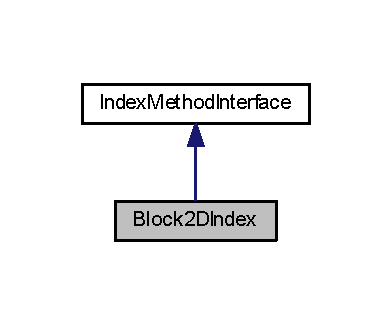
\includegraphics[width=188pt]{class_block2_d_index__inherit__graph}
\end{center}
\end{figure}


Block2\-D\-Index 的协作图\-:\nopagebreak
\begin{figure}[H]
\begin{center}
\leavevmode
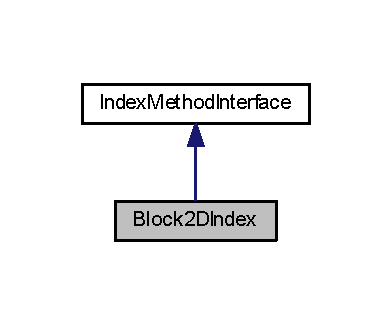
\includegraphics[width=188pt]{class_block2_d_index__coll__graph}
\end{center}
\end{figure}
\subsection*{Public 成员函数}
\begin{DoxyCompactItemize}
\item 
{\bf Block2\-D\-Index} ({\bf Index\-Type} row\-\_\-size, {\bf Index\-Type} col\-\_\-size, {\bf Index\-Type} block\-\_\-row\-\_\-size, {\bf Index\-Type} block\-\_\-col\-\_\-size=-\/1)
\item 
virtual {\bf Index\-Type} {\bf get\-\_\-index} ({\bf Row\-Major\-Index\-Type} row\-\_\-index, {\bf Row\-Major\-Index\-Type} col\-\_\-index) const \label{class_block2_d_index_a0dfd01476ef2edd3c827169460cd881f}

\begin{DoxyCompactList}\small\item\em get the index of row-\/major index (row, col) \end{DoxyCompactList}\item 
virtual {\bf Row\-Major\-Point} {\bf get\-\_\-origin\-\_\-index} ({\bf Index\-Type} index) const 
\begin{DoxyCompactList}\small\item\em get the original row-\/major index \end{DoxyCompactList}\item 
virtual {\bf Index\-Type} {\bf get\-\_\-row\-\_\-result} ({\bf Row\-Major\-Index\-Type} row\-\_\-index) const 
\begin{DoxyCompactList}\small\item\em get the row result from just the row index (for using row-\/major like loop). \end{DoxyCompactList}\item 
virtual {\bf Index\-Type} {\bf get\-\_\-index\-\_\-by\-\_\-row\-\_\-result} ({\bf Index\-Type} row\-\_\-result, {\bf Row\-Major\-Index\-Type} col\-\_\-index) const 
\begin{DoxyCompactList}\small\item\em get the index from row result and col index \end{DoxyCompactList}\item 
virtual {\bf Index\-Type} {\bf get\-\_\-max\-\_\-index} () const 
\begin{DoxyCompactList}\small\item\em get the maximum index, often used to ensure the size of the container \end{DoxyCompactList}\item 
virtual std\-::string {\bf get\-\_\-index\-\_\-method\-\_\-name} () const \label{class_block2_d_index_afc8180e499be3f40ff94ec4bbf2eeed2}

\begin{DoxyCompactList}\small\item\em get the index method name for identify different method \end{DoxyCompactList}\item 
{\bf Index\-Type} {\bfseries get\-Block\-Row\-Count} () const \label{class_block2_d_index_ac54aa06997034860186fb1e65e7a3ab2}

\item 
{\bf Index\-Type} {\bfseries get\-Block\-Col\-Count} () const \label{class_block2_d_index_a47dda65ea5127b752c1b021bb150bb0b}

\item 
{\bf Index\-Type} {\bfseries get\-Block\-Total\-Size} () const \label{class_block2_d_index_aa9b6423a81a8232212317c488c619cca}

\item 
{\bf Index\-Type} {\bfseries get\-Block\-Row\-Size} () const \label{class_block2_d_index_a2fd9216fdf64b7445845900845482392}

\item 
{\bf Index\-Type} {\bfseries get\-Block\-Col\-Size} () const \label{class_block2_d_index_a4581d3068dc26ff731557a418311549b}

\end{DoxyCompactItemize}
\subsection*{额外继承的成员函数}


\subsection{详细描述}
\begin{Desc}
\item[示例\-: ]\par
{\bf test\-Index\-Method.\-cpp}.\end{Desc}


在文件 {\bf Index\-Method.\-hpp} 第  行定义.



\subsection{构造及析构函数说明}
\index{Block2\-D\-Index@{Block2\-D\-Index}!Block2\-D\-Index@{Block2\-D\-Index}}
\index{Block2\-D\-Index@{Block2\-D\-Index}!Block2DIndex@{Block2\-D\-Index}}
\subsubsection[{Block2\-D\-Index}]{\setlength{\rightskip}{0pt plus 5cm}Block2\-D\-Index\-::\-Block2\-D\-Index (
\begin{DoxyParamCaption}
\item[{{\bf Index\-Type}}]{row\-\_\-size, }
\item[{{\bf Index\-Type}}]{col\-\_\-size, }
\item[{{\bf Index\-Type}}]{block\-\_\-row\-\_\-size, }
\item[{{\bf Index\-Type}}]{block\-\_\-col\-\_\-size = {\ttfamily -\/1}}
\end{DoxyParamCaption}
)\hspace{0.3cm}{\ttfamily [inline]}}\label{class_block2_d_index_a976f95172bf060f3abd3c4f776069d72}

\begin{DoxyParams}{参数}
{\em row\-\_\-size} & the row size of the image \\
\hline
{\em col\-\_\-size} & the col size of the image \\
\hline
{\em block\-\_\-row\-\_\-size} & the row size of the block in the unit of 2$^\wedge$n, \\
\hline
{\em block\-\_\-col\-\_\-size} & the col size of the block in the unit of 2$^\wedge$n. If n = 2, then the block size is 4 \\
\hline
\end{DoxyParams}


在文件 {\bf Index\-Method.\-hpp} 第  行定义.



\subsection{成员函数说明}
\index{Block2\-D\-Index@{Block2\-D\-Index}!get\-\_\-index\-\_\-by\-\_\-row\-\_\-result@{get\-\_\-index\-\_\-by\-\_\-row\-\_\-result}}
\index{get\-\_\-index\-\_\-by\-\_\-row\-\_\-result@{get\-\_\-index\-\_\-by\-\_\-row\-\_\-result}!Block2DIndex@{Block2\-D\-Index}}
\subsubsection[{get\-\_\-index\-\_\-by\-\_\-row\-\_\-result}]{\setlength{\rightskip}{0pt plus 5cm}virtual {\bf Index\-Type} Block2\-D\-Index\-::get\-\_\-index\-\_\-by\-\_\-row\-\_\-result (
\begin{DoxyParamCaption}
\item[{{\bf Index\-Type}}]{row\-\_\-result, }
\item[{{\bf Row\-Major\-Index\-Type}}]{col\-\_\-index}
\end{DoxyParamCaption}
) const\hspace{0.3cm}{\ttfamily [inline]}, {\ttfamily [virtual]}}\label{class_block2_d_index_a3ead3723b1619b13e20a4ed14469a32d}


get the index from row result and col index 


\begin{DoxyParams}{参数}
{\em row\-\_\-result} & the result get from the \doxyref{get\-\_\-row\-\_\-result()}{p.}{class_block2_d_index_a96c5893d835bf952463cef1398654361} method \\
\hline
{\em col\-\_\-index} & the index of col in the row-\/major format \\
\hline
\end{DoxyParams}
\begin{DoxyReturn}{返回}
the index result combined both the row and col 
\end{DoxyReturn}


实现了 {\bf Index\-Method\-Interface} \doxyref{}{p.}{class_index_method_interface_af6fda6db139d00aa3e722fcd20945322}.

\begin{Desc}
\item[示例\-: ]\par
{\bf test\-Index\-Method.\-cpp}.\end{Desc}


在文件 {\bf Index\-Method.\-hpp} 第  行定义.

\index{Block2\-D\-Index@{Block2\-D\-Index}!get\-\_\-max\-\_\-index@{get\-\_\-max\-\_\-index}}
\index{get\-\_\-max\-\_\-index@{get\-\_\-max\-\_\-index}!Block2DIndex@{Block2\-D\-Index}}
\subsubsection[{get\-\_\-max\-\_\-index}]{\setlength{\rightskip}{0pt plus 5cm}virtual {\bf Index\-Type} Block2\-D\-Index\-::get\-\_\-max\-\_\-index (
\begin{DoxyParamCaption}
{}
\end{DoxyParamCaption}
) const\hspace{0.3cm}{\ttfamily [inline]}, {\ttfamily [virtual]}}\label{class_block2_d_index_a1cdb7f2f1ca93be4e14cee70f4038160}


get the maximum index, often used to ensure the size of the container 

\begin{DoxyReturn}{返回}
the maximum index get from the this indexing method 
\end{DoxyReturn}


实现了 {\bf Index\-Method\-Interface} \doxyref{}{p.}{class_index_method_interface_ad2e684fc1ef5ea505ccbc23278977478}.

\begin{Desc}
\item[示例\-: ]\par
{\bf test\-Index\-Method.\-cpp}.\end{Desc}


在文件 {\bf Index\-Method.\-hpp} 第  行定义.

\index{Block2\-D\-Index@{Block2\-D\-Index}!get\-\_\-origin\-\_\-index@{get\-\_\-origin\-\_\-index}}
\index{get\-\_\-origin\-\_\-index@{get\-\_\-origin\-\_\-index}!Block2DIndex@{Block2\-D\-Index}}
\subsubsection[{get\-\_\-origin\-\_\-index}]{\setlength{\rightskip}{0pt plus 5cm}virtual {\bf Row\-Major\-Point} Block2\-D\-Index\-::get\-\_\-origin\-\_\-index (
\begin{DoxyParamCaption}
\item[{{\bf Index\-Type}}]{index}
\end{DoxyParamCaption}
) const\hspace{0.3cm}{\ttfamily [inline]}, {\ttfamily [virtual]}}\label{class_block2_d_index_a95e1c7406cabbcf2decde099128a6fa5}


get the original row-\/major index 


\begin{DoxyParams}{参数}
{\em index} & the index calculated from \doxyref{get\-\_\-index()}{p.}{class_block2_d_index_a0dfd01476ef2edd3c827169460cd881f} method \\
\hline
\end{DoxyParams}
\begin{DoxyReturn}{返回}
the row-\/major index (row, col) format 
\end{DoxyReturn}


实现了 {\bf Index\-Method\-Interface} \doxyref{}{p.}{class_index_method_interface_a44f4553bd06c787d4523c37a9a15fdd3}.

\begin{Desc}
\item[示例\-: ]\par
{\bf test\-Index\-Method.\-cpp}.\end{Desc}


在文件 {\bf Index\-Method.\-hpp} 第  行定义.

\index{Block2\-D\-Index@{Block2\-D\-Index}!get\-\_\-row\-\_\-result@{get\-\_\-row\-\_\-result}}
\index{get\-\_\-row\-\_\-result@{get\-\_\-row\-\_\-result}!Block2DIndex@{Block2\-D\-Index}}
\subsubsection[{get\-\_\-row\-\_\-result}]{\setlength{\rightskip}{0pt plus 5cm}virtual {\bf Index\-Type} Block2\-D\-Index\-::get\-\_\-row\-\_\-result (
\begin{DoxyParamCaption}
\item[{{\bf Row\-Major\-Index\-Type}}]{row\-\_\-index}
\end{DoxyParamCaption}
) const\hspace{0.3cm}{\ttfamily [inline]}, {\ttfamily [virtual]}}\label{class_block2_d_index_a96c5893d835bf952463cef1398654361}


get the row result from just the row index (for using row-\/major like loop). 


\begin{DoxyPre}
Using this method for some kind of optimization when using row-major like loop 
for example:    
for(size\_t row = 0; row < rows; ++row) \{ 
        IndexType row\_result = get\_row\_result(row);
        for(size\_t col = 0; col < cols; ++col) \{ 
                IndexType index = get\_index\_by\_row\_result(row\_result, col); 
        \} 
\} 
\end{DoxyPre}



\begin{DoxyParams}{参数}
{\em row\-\_\-index} & the index of row in the row-\/major format \\
\hline
\end{DoxyParams}
\begin{DoxyReturn}{返回}
the row result 
\end{DoxyReturn}


实现了 {\bf Index\-Method\-Interface} \doxyref{}{p.}{class_index_method_interface_aab87157a6dcd40f8d249616829f7ec97}.

\begin{Desc}
\item[示例\-: ]\par
{\bf test\-Index\-Method.\-cpp}.\end{Desc}


在文件 {\bf Index\-Method.\-hpp} 第  行定义.



该类的文档由以下文件生成\-:\begin{DoxyCompactItemize}
\item 
D\-:/\-Out\-\_\-\-Of\-\_\-\-Core\-\_\-\-Git/src/Index\-Method.\-hpp\end{DoxyCompactItemize}

\section{Blockwise\-Image$<$ T, memory\-\_\-usage $>$ 模板类 参考}
\label{class_blockwise_image}\index{Blockwise\-Image$<$ T, memory\-\_\-usage $>$@{Blockwise\-Image$<$ T, memory\-\_\-usage $>$}}


Derived from \doxyref{Giant\-Image\-Interface}{p.}{class_giant_image_interface}, support the big image operation, and saves the whole image into disk.  




{\ttfamily \#include $<$Blockwise\-Image.\-h$>$}



类 Blockwise\-Image$<$ T, memory\-\_\-usage $>$ 继承关系图\-:\nopagebreak
\begin{figure}[H]
\begin{center}
\leavevmode
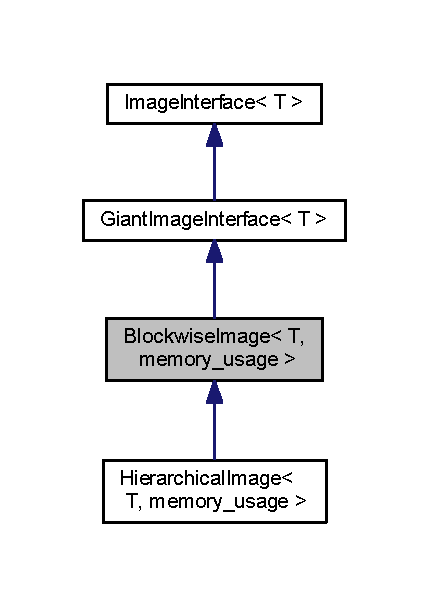
\includegraphics[width=206pt]{class_blockwise_image__inherit__graph}
\end{center}
\end{figure}


Blockwise\-Image$<$ T, memory\-\_\-usage $>$ 的协作图\-:\nopagebreak
\begin{figure}[H]
\begin{center}
\leavevmode
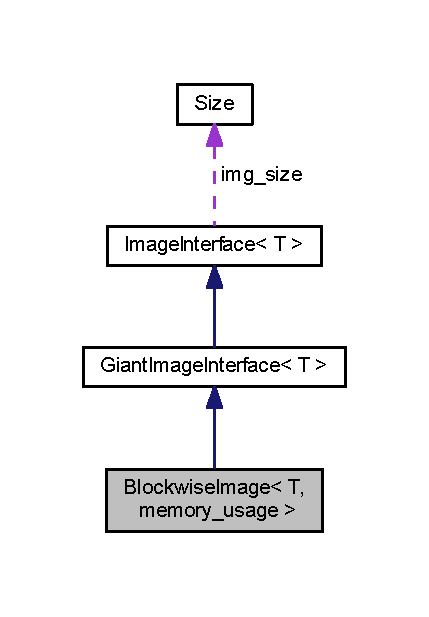
\includegraphics[width=206pt]{class_blockwise_image__coll__graph}
\end{center}
\end{figure}
\subsection*{Public 成员函数}
\begin{DoxyCompactItemize}
\item 
{\bf Blockwise\-Image} (int rows, int cols, int mini\-\_\-rows, int mini\-\_\-cols, boost\-::shared\-\_\-ptr$<$ {\bf Index\-Method\-Interface} $>$ method=boost\-::shared\-\_\-ptr$<$ {\bf Index\-Method\-Interface} $>$())
\begin{DoxyCompactList}\small\item\em get the blockwise image container according to the image size. \end{DoxyCompactList}\item 
virtual bool {\bf init} (int rows, int cols)
\begin{DoxyCompactList}\small\item\em Initialize the image size, and allocate the memory for saving the image. \end{DoxyCompactList}\item 
virtual bool {\bf reset} ()\label{class_blockwise_image_ac83f27ff25be2a0c5ba9b1e8c5494846}

\begin{DoxyCompactList}\small\item\em Clear the image data. \end{DoxyCompactList}\item 
virtual bool {\bf write\-\_\-image} (const char $\ast$file\-\_\-name)
\item 
virtual bool {\bfseries write\-\_\-image} (const std\-::string \&file\-\_\-name)\label{class_blockwise_image_a6f0b01bdb2ed0bd2db958a64a789c037}

\item 
virtual T \& {\bf get\-\_\-pixel} (int row, int col)
\begin{DoxyCompactList}\small\item\em Get the pixel of the point (row, col), or just write code like image(row, col) to get the image pixel. \end{DoxyCompactList}\item 
virtual const T \& {\bfseries get\-\_\-pixel} (int row, int col) const \label{class_blockwise_image_a045e63f79945bb116b30a8b5af7f7f9f}

\item 
virtual T \& {\bfseries operator()} (int row, int col)\label{class_blockwise_image_a36d10d899536d963b826458e01220aba}

\item 
virtual const T \& {\bfseries operator()} (int row, int col) const \label{class_blockwise_image_ad244c3ec3b36090f3ec51b350c792b79}

\item 
virtual bool {\bf get\-\_\-pixels} (int start\-\_\-row, int start\-\_\-col, int rows, int cols, std\-::vector$<$ T $>$ \&data) const 
\begin{DoxyCompactList}\small\item\em Get the range image data. \end{DoxyCompactList}\item 
virtual bool {\bfseries set\-\_\-pixels} (int start\-\_\-row, int start\-\_\-col, int rows, int cols, const std\-::vector$<$ T $>$ \&data)\label{class_blockwise_image_a70d170f7869795a2453504ddc07a6e1b}

\item 
virtual bool {\bf set\-\_\-pixels} (int start\-\_\-row, int start\-\_\-col, int rows, int cols, const T clear\-\_\-value)
\begin{DoxyCompactList}\small\item\em set the range image data with a const value \end{DoxyCompactList}\item 
virtual T \& {\bf at} ({\bf Index\-Method\-Interface\-::\-Index\-Type} index)
\begin{DoxyCompactList}\small\item\em get the element by the one dimension index \end{DoxyCompactList}\item 
virtual const T \& {\bfseries at} ({\bf Index\-Method\-Interface\-::\-Index\-Type} index) const \label{class_blockwise_image_a4c30fa98f972a78b6d36c3960b6dc286}

\item 
size\-\_\-t {\bf get\-\_\-minimal\-\_\-image\-\_\-rows} () const \label{class_blockwise_image_ad9853076b2ab7449a6084e4816d1dad0}

\begin{DoxyCompactList}\small\item\em \-: get the minimum image size \end{DoxyCompactList}\item 
size\-\_\-t {\bfseries get\-\_\-minimal\-\_\-image\-\_\-cols} () const \label{class_blockwise_image_a2bf6dda12d1b1dafd5ee347ba42e35a3}

\item 
size\-\_\-t {\bf get\-\_\-max\-\_\-image\-\_\-level} () const \label{class_blockwise_image_aeb1827b1d6fb7df33b52ca25e3707a18}

\begin{DoxyCompactList}\small\item\em \-: get the maximum image level \end{DoxyCompactList}\end{DoxyCompactItemize}
\subsection*{Protected 类型}
\begin{DoxyCompactItemize}
\item 
typedef stxxl\-::vector$<$ T, \\*
4, stxxl\-::lru\-\_\-pager\\*
$<$(memory\-\_\-usage $>$$>$ 3)$>$ $>$ {\bf Container\-Type}
\begin{DoxyCompactList}\small\item\em saves the image data in the disk. \end{DoxyCompactList}\end{DoxyCompactItemize}
\subsection*{Protected 成员函数}
\begin{DoxyCompactItemize}
\item 
bool {\bf write\-\_\-image\-\_\-head\-\_\-file} (const char $\ast$file\-\_\-name)\label{class_blockwise_image_ad77dc700826b65cb0d4b3ca0ea586b2a}

\begin{DoxyCompactList}\small\item\em \-: write the image head info before write the actual image data \end{DoxyCompactList}\item 
void {\bf set\-\_\-minimal\-\_\-resolution} (int rows, int cols, int mini\-\_\-rows, int mini\-\_\-cols)
\begin{DoxyCompactList}\small\item\em \-: set the minimum image size according to the image size (rows, cols). \end{DoxyCompactList}\item 
virtual bool {\bf save\-\_\-mini\-\_\-image} (const char $\ast$file\-\_\-name)
\begin{DoxyCompactList}\small\item\em save the mini size image as a jpg file for observation \end{DoxyCompactList}\end{DoxyCompactItemize}
\subsection*{Protected 属性}
\begin{DoxyCompactItemize}
\item 
{\bf Container\-Type} {\bfseries img\-\_\-container}\label{class_blockwise_image_aec3ffc3c2e93dd905001c396de5a0631}

\item 
size\-\_\-t {\bfseries m\-\_\-mini\-\_\-rows}\label{class_blockwise_image_a5dfb1d1e5a4f25973024064eaef2b30b}

\item 
size\-\_\-t {\bfseries m\-\_\-mini\-\_\-cols}\label{class_blockwise_image_a7759da621d38319d1135acc5bfb1d37a}

\item 
size\-\_\-t {\bfseries m\-\_\-max\-\_\-level}\label{class_blockwise_image_a0d45e5ad80f47684727df0d8021b7050}

\end{DoxyCompactItemize}
\subsection*{相关函数}
(请注意\-: 这些不是成员函数.) \begin{DoxyCompactItemize}
\item 
{\footnotesize template$<$typename T $>$ }\\boost\-::shared\-\_\-ptr\\*
$<$ {\bf Giant\-Image\-Interface}$<$ T $>$ $>$ {\bf get\-\_\-block\-\_\-wise\-\_\-image\-\_\-by\-\_\-meomory\-\_\-usage} (unsigned memory\-\_\-usage, size\-\_\-t rows, size\-\_\-t cols, size\-\_\-t mini\-\_\-rows, size\-\_\-t mini\-\_\-cols, boost\-::shared\-\_\-ptr$<$ {\bf Index\-Method\-Interface} $>$ method=boost\-::shared\-\_\-ptr$<$ {\bf Index\-Method\-Interface} $>$())
\begin{DoxyCompactList}\small\item\em return the block wise image by memroy\-\_\-usage, maximum support 4\-G. \end{DoxyCompactList}\end{DoxyCompactItemize}


\subsection{详细描述}
\subsubsection*{template$<$typename T, unsigned memory\-\_\-usage = 64$>$class Blockwise\-Image$<$ T, memory\-\_\-usage $>$}

Derived from \doxyref{Giant\-Image\-Interface}{p.}{class_giant_image_interface}, support the big image operation, and saves the whole image into disk. 

\doxyref{Blockwise\-Image}{p.}{class_blockwise_image} can support very big image processing and storing, and can be wrote into the disk in a non compressed way.


\begin{DoxyTemplParams}{Template Parameters}
{\em T} & The type of the image cell \\
\hline
{\em memory\-\_\-usage} & The memory usage used as a I/\-O cache in the main memory, and it must be bigger than 8 (in the unit of M). By default, memory\-\_\-usage is set to 64\-M \\
\hline
\end{DoxyTemplParams}
\begin{Desc}
\item[示例\-: ]\par
{\bf Write\-Block\-Wise\-Image.\-cpp}.\end{Desc}


在文件 {\bf Blockwise\-Image.\-h} 第  行定义.



\subsection{成员类型定义说明}
\index{Blockwise\-Image@{Blockwise\-Image}!Container\-Type@{Container\-Type}}
\index{Container\-Type@{Container\-Type}!BlockwiseImage@{Blockwise\-Image}}
\subsubsection[{Container\-Type}]{\setlength{\rightskip}{0pt plus 5cm}template$<$typename T , unsigned memory\-\_\-usage = 64$>$ typedef stxxl\-::vector$<$T, 4, stxxl\-::lru\-\_\-pager$<$(memory\-\_\-usage $>$$>$ 3)$>$ $>$ {\bf Blockwise\-Image}$<$ T, memory\-\_\-usage $>$\-::{\bf Container\-Type}\hspace{0.3cm}{\ttfamily [protected]}}\label{class_blockwise_image_a3bc3cd5a61a801c45fa6523f2865d056}


saves the image data in the disk. 

4 means a page has 4 blocks lru\-\_\-pages$<$n$>$ \-: n means the number of pages in memory each block is 2\-M , thus total memroy usage = 8\-M $\ast$ (number of pages) , thus why right shift 3 bit 

在文件 {\bf Blockwise\-Image.\-h} 第  行定义.



\subsection{构造及析构函数说明}
\index{Blockwise\-Image@{Blockwise\-Image}!Blockwise\-Image@{Blockwise\-Image}}
\index{Blockwise\-Image@{Blockwise\-Image}!BlockwiseImage@{Blockwise\-Image}}
\subsubsection[{Blockwise\-Image}]{\setlength{\rightskip}{0pt plus 5cm}template$<$typename T , unsigned memory\-\_\-usage$>$ {\bf Blockwise\-Image}$<$ T, memory\-\_\-usage $>$\-::{\bf Blockwise\-Image} (
\begin{DoxyParamCaption}
\item[{int}]{rows, }
\item[{int}]{cols, }
\item[{int}]{mini\-\_\-rows, }
\item[{int}]{mini\-\_\-cols, }
\item[{boost\-::shared\-\_\-ptr$<$ {\bf Index\-Method\-Interface} $>$}]{method = {\ttfamily boost\-:\-:shared\-\_\-ptr$<${\bf Index\-Method\-Interface}$>$()}}
\end{DoxyParamCaption}
)}\label{class_blockwise_image_a47d9836eb6f1544d5557234f2616c757}


get the blockwise image container according to the image size. 

After write the image into the filesystem, a minimum size image will be saved in the disk as a jpg file format, so the constructor needs the minimum image size information


\begin{DoxyParams}{参数}
{\em rows} & the image rows \\
\hline
{\em cols} & the image cols \\
\hline
{\em mini\-\_\-rows} & the minimum rows of the image \\
\hline
{\em mini\-\_\-cols} & the minimum cols of the image \\
\hline
{\em method} & the index method shared\-\_\-ptr object(default is zorder index method) \\
\hline
\end{DoxyParams}


在文件 {\bf Blockwise\-Image.\-hpp} 第  行定义.



函数调用图\-:\nopagebreak
\begin{figure}[H]
\begin{center}
\leavevmode
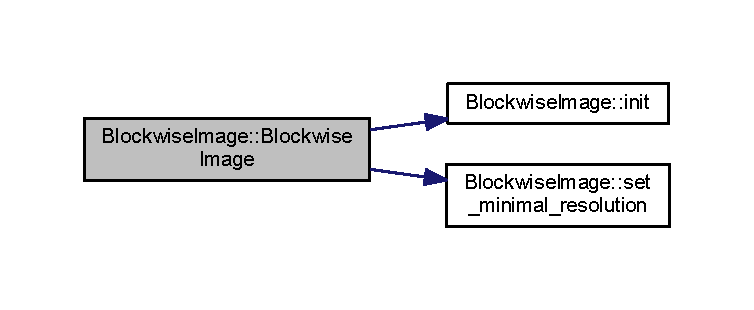
\includegraphics[width=350pt]{class_blockwise_image_a47d9836eb6f1544d5557234f2616c757_cgraph}
\end{center}
\end{figure}




\subsection{成员函数说明}
\index{Blockwise\-Image@{Blockwise\-Image}!at@{at}}
\index{at@{at}!BlockwiseImage@{Blockwise\-Image}}
\subsubsection[{at}]{\setlength{\rightskip}{0pt plus 5cm}template$<$typename T , unsigned memory\-\_\-usage$>$ T \& {\bf Blockwise\-Image}$<$ T, memory\-\_\-usage $>$\-::at (
\begin{DoxyParamCaption}
\item[{{\bf Index\-Method\-Interface\-::\-Index\-Type}}]{index}
\end{DoxyParamCaption}
)\hspace{0.3cm}{\ttfamily [virtual]}}\label{class_blockwise_image_ab0cf952a4b988f8735dc770d9b0c787b}


get the element by the one dimension index 


\begin{DoxyParams}{参数}
{\em index} & one dimension index \\
\hline
\end{DoxyParams}


实现了 {\bf Giant\-Image\-Interface$<$ T $>$} \doxyref{}{p.}{class_giant_image_interface_a1f98aece25249d626e60ebb9b0f05111}.



在文件 {\bf Blockwise\-Image.\-hpp} 第  行定义.

\index{Blockwise\-Image@{Blockwise\-Image}!get\-\_\-pixel@{get\-\_\-pixel}}
\index{get\-\_\-pixel@{get\-\_\-pixel}!BlockwiseImage@{Blockwise\-Image}}
\subsubsection[{get\-\_\-pixel}]{\setlength{\rightskip}{0pt plus 5cm}template$<$typename T , unsigned memory\-\_\-usage$>$ T \& {\bf Blockwise\-Image}$<$ T, memory\-\_\-usage $>$\-::get\-\_\-pixel (
\begin{DoxyParamCaption}
\item[{int}]{row, }
\item[{int}]{col}
\end{DoxyParamCaption}
)\hspace{0.3cm}{\ttfamily [virtual]}}\label{class_blockwise_image_a110d2b1c0d6ac08cb8e66f74b32bd72d}


Get the pixel of the point (row, col), or just write code like image(row, col) to get the image pixel. 

\begin{DoxyReturn}{返回}
The reference of the image pixel 
\end{DoxyReturn}
\begin{DoxyWarning}{警告}
In release mode, the row and col param must be valid, otherwise there will be an exception 
\end{DoxyWarning}


实现了 {\bf Image\-Interface$<$ T $>$} \doxyref{}{p.}{class_image_interface_af5fc491e3c7bb401a3591de26049bc7d}.



在文件 {\bf Blockwise\-Image.\-hpp} 第  行定义.

\index{Blockwise\-Image@{Blockwise\-Image}!get\-\_\-pixels@{get\-\_\-pixels}}
\index{get\-\_\-pixels@{get\-\_\-pixels}!BlockwiseImage@{Blockwise\-Image}}
\subsubsection[{get\-\_\-pixels}]{\setlength{\rightskip}{0pt plus 5cm}template$<$typename T , unsigned memory\-\_\-usage$>$ bool {\bf Blockwise\-Image}$<$ T, memory\-\_\-usage $>$\-::get\-\_\-pixels (
\begin{DoxyParamCaption}
\item[{int}]{start\-\_\-row, }
\item[{int}]{start\-\_\-col, }
\item[{int}]{rows, }
\item[{int}]{cols, }
\item[{std\-::vector$<$ T $>$ \&}]{data}
\end{DoxyParamCaption}
) const\hspace{0.3cm}{\ttfamily [virtual]}}\label{class_blockwise_image_a91c1d0be2ef9ab54f1a5f9e706e13174}


Get the range image data. 


\begin{DoxyParams}{参数}
{\em start\-\_\-row} & The left-\/corner point row \\
\hline
{\em start\-\_\-col} & The left-\/corner point col \\
\hline
{\em rows} & The row scope of the range, thus the rows get is [start\-\_\-row, start\-\_\-row + rows) \\
\hline
{\em cols} & The col scope of the range \\
\hline
{\em data} & [Out] Returns the image data vector \\
\hline
\end{DoxyParams}
\begin{DoxyNote}{注解}
the data doesn't need to allocate any memory 
\end{DoxyNote}
\begin{DoxyReturn}{返回}
Whether get the data successfully 
\end{DoxyReturn}


实现了 {\bf Image\-Interface$<$ T $>$} \doxyref{}{p.}{class_image_interface_a2a2254be220b4a4bb6effed70d61c6df}.



在文件 {\bf Blockwise\-Image.\-hpp} 第  行定义.

\index{Blockwise\-Image@{Blockwise\-Image}!init@{init}}
\index{init@{init}!BlockwiseImage@{Blockwise\-Image}}
\subsubsection[{init}]{\setlength{\rightskip}{0pt plus 5cm}template$<$typename T , unsigned memory\-\_\-usage$>$ bool {\bf Blockwise\-Image}$<$ T, memory\-\_\-usage $>$\-::init (
\begin{DoxyParamCaption}
\item[{int}]{rows, }
\item[{int}]{cols}
\end{DoxyParamCaption}
)\hspace{0.3cm}{\ttfamily [virtual]}}\label{class_blockwise_image_a9bbeb6df0a51caf818d100c3e869f45b}


Initialize the image size, and allocate the memory for saving the image. 

\begin{DoxyReturn}{返回}
Whether initialize successfully 
\end{DoxyReturn}


实现了 {\bf Image\-Interface$<$ T $>$} \doxyref{}{p.}{class_image_interface_a6f59d1e81ab88e0ca2c5d4b6a2e98ae5}.



在文件 {\bf Blockwise\-Image.\-hpp} 第  行定义.



这是这个函数的调用关系图\-:\nopagebreak
\begin{figure}[H]
\begin{center}
\leavevmode
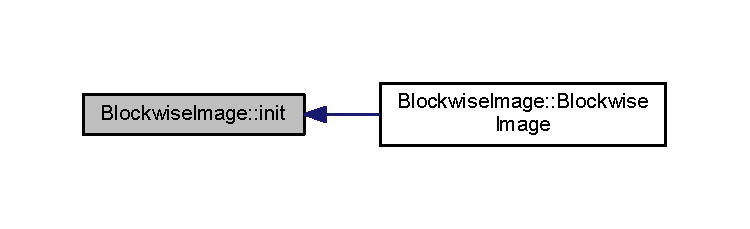
\includegraphics[width=350pt]{class_blockwise_image_a9bbeb6df0a51caf818d100c3e869f45b_icgraph}
\end{center}
\end{figure}


\index{Blockwise\-Image@{Blockwise\-Image}!save\-\_\-mini\-\_\-image@{save\-\_\-mini\-\_\-image}}
\index{save\-\_\-mini\-\_\-image@{save\-\_\-mini\-\_\-image}!BlockwiseImage@{Blockwise\-Image}}
\subsubsection[{save\-\_\-mini\-\_\-image}]{\setlength{\rightskip}{0pt plus 5cm}template$<$typename T , unsigned memory\-\_\-usage$>$ bool {\bf Blockwise\-Image}$<$ T, memory\-\_\-usage $>$\-::save\-\_\-mini\-\_\-image (
\begin{DoxyParamCaption}
\item[{const char $\ast$}]{file\-\_\-name}
\end{DoxyParamCaption}
)\hspace{0.3cm}{\ttfamily [protected]}, {\ttfamily [virtual]}}\label{class_blockwise_image_a47ca8a383348f9cc527365977e9d721b}


save the mini size image as a jpg file for observation 


\begin{DoxyParams}{参数}
{\em file\-\_\-name} & the bigimage file name ($\ast$.bigimage) \\
\hline
\end{DoxyParams}
\begin{DoxyNote}{注解}
if not defined the S\-A\-V\-E\-\_\-\-M\-I\-N\-I\-\_\-\-I\-M\-A\-G\-E macro, this function will do nothing 
\end{DoxyNote}


被 {\bf Hierarchical\-Image$<$ T, memory\-\_\-usage $>$} \doxyref{}{p.}{class_hierarchical_image_ad4c49535e55585ed7726856d8c65ef6e} 重载.



在文件 {\bf Blockwise\-Image.\-hpp} 第  行定义.

\index{Blockwise\-Image@{Blockwise\-Image}!set\-\_\-minimal\-\_\-resolution@{set\-\_\-minimal\-\_\-resolution}}
\index{set\-\_\-minimal\-\_\-resolution@{set\-\_\-minimal\-\_\-resolution}!BlockwiseImage@{Blockwise\-Image}}
\subsubsection[{set\-\_\-minimal\-\_\-resolution}]{\setlength{\rightskip}{0pt plus 5cm}template$<$typename T , unsigned memory\-\_\-usage$>$ void {\bf Blockwise\-Image}$<$ T, memory\-\_\-usage $>$\-::set\-\_\-minimal\-\_\-resolution (
\begin{DoxyParamCaption}
\item[{int}]{rows, }
\item[{int}]{cols, }
\item[{int}]{mini\-\_\-rows, }
\item[{int}]{mini\-\_\-cols}
\end{DoxyParamCaption}
)\hspace{0.3cm}{\ttfamily [protected]}}\label{class_blockwise_image_a24fcb54429ce4d5df42532115b17d3ec}


\-: set the minimum image size according to the image size (rows, cols). 

The minimum image size is set according to the principle \-: the mini image size$\ast$2$^\wedge$n = total image size


\begin{DoxyParams}{参数}
{\em rows} & the image rows \\
\hline
{\em cols} & the image cols \\
\hline
{\em mini\-\_\-rows} & the minimum rows of the image \\
\hline
{\em mini\-\_\-cols} & the minimum cols of the image \\
\hline
\end{DoxyParams}


在文件 {\bf Blockwise\-Image.\-hpp} 第  行定义.



这是这个函数的调用关系图\-:\nopagebreak
\begin{figure}[H]
\begin{center}
\leavevmode
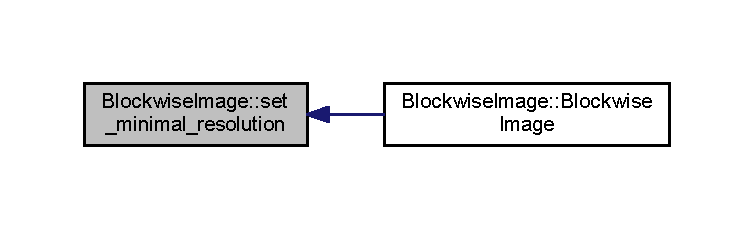
\includegraphics[width=350pt]{class_blockwise_image_a24fcb54429ce4d5df42532115b17d3ec_icgraph}
\end{center}
\end{figure}


\index{Blockwise\-Image@{Blockwise\-Image}!set\-\_\-pixels@{set\-\_\-pixels}}
\index{set\-\_\-pixels@{set\-\_\-pixels}!BlockwiseImage@{Blockwise\-Image}}
\subsubsection[{set\-\_\-pixels}]{\setlength{\rightskip}{0pt plus 5cm}template$<$typename T , unsigned memory\-\_\-usage$>$ bool {\bf Blockwise\-Image}$<$ T, memory\-\_\-usage $>$\-::set\-\_\-pixels (
\begin{DoxyParamCaption}
\item[{int}]{start\-\_\-row, }
\item[{int}]{start\-\_\-col, }
\item[{int}]{rows, }
\item[{int}]{cols, }
\item[{const T}]{clear\-\_\-value}
\end{DoxyParamCaption}
)\hspace{0.3cm}{\ttfamily [virtual]}}\label{class_blockwise_image_ac4da5390aa20631c1f0e88b6a93cfead}


set the range image data with a const value 


\begin{DoxyParams}{参数}
{\em start\-\_\-row} & The left-\/corner point row \\
\hline
{\em start\-\_\-col} & The left-\/corner point col \\
\hline
{\em rows} & The row scope of the range, thus the rows get is [start\-\_\-row, start\-\_\-row + rows) \\
\hline
{\em cols} & The col scope of the range \\
\hline
{\em clear\-\_\-value} & the value that with to fill the image range \\
\hline
\end{DoxyParams}
\begin{DoxyReturn}{返回}
Whether set successfully 
\end{DoxyReturn}


实现了 {\bf Image\-Interface$<$ T $>$} \doxyref{}{p.}{class_image_interface_aa35f6a2c062df7a9796fc672b16cafc8}.



在文件 {\bf Blockwise\-Image.\-hpp} 第  行定义.

\index{Blockwise\-Image@{Blockwise\-Image}!write\-\_\-image@{write\-\_\-image}}
\index{write\-\_\-image@{write\-\_\-image}!BlockwiseImage@{Blockwise\-Image}}
\subsubsection[{write\-\_\-image}]{\setlength{\rightskip}{0pt plus 5cm}template$<$typename T , unsigned memory\-\_\-usage$>$ bool {\bf Blockwise\-Image}$<$ T, memory\-\_\-usage $>$\-::write\-\_\-image (
\begin{DoxyParamCaption}
\item[{const char $\ast$}]{file\-\_\-name}
\end{DoxyParamCaption}
)\hspace{0.3cm}{\ttfamily [virtual]}}\label{class_blockwise_image_a64f3e966d516c8b039bd9f4c8685055c}
\begin{DoxyNote}{注解}
file\-\_\-name must has the extension \char`\"{}.\-bigimage\char`\"{} 
\end{DoxyNote}


实现了 {\bf Image\-Interface$<$ T $>$} \doxyref{}{p.}{class_image_interface_ad5c2431a4b31bcb600ba996858efa620}.



被 {\bf Hierarchical\-Image$<$ T, memory\-\_\-usage $>$} \doxyref{}{p.}{class_hierarchical_image_a6ade13ae295516b5a899498c6800451d} 重载.



在文件 {\bf Blockwise\-Image.\-hpp} 第  行定义.



\subsection{友元及相关函数文档}
\index{Blockwise\-Image@{Blockwise\-Image}!get\-\_\-block\-\_\-wise\-\_\-image\-\_\-by\-\_\-meomory\-\_\-usage@{get\-\_\-block\-\_\-wise\-\_\-image\-\_\-by\-\_\-meomory\-\_\-usage}}
\index{get\-\_\-block\-\_\-wise\-\_\-image\-\_\-by\-\_\-meomory\-\_\-usage@{get\-\_\-block\-\_\-wise\-\_\-image\-\_\-by\-\_\-meomory\-\_\-usage}!BlockwiseImage@{Blockwise\-Image}}
\subsubsection[{get\-\_\-block\-\_\-wise\-\_\-image\-\_\-by\-\_\-meomory\-\_\-usage}]{\setlength{\rightskip}{0pt plus 5cm}template$<$typename T $>$ boost\-::shared\-\_\-ptr$<$ {\bf Giant\-Image\-Interface}$<$ T $>$ $>$ get\-\_\-block\-\_\-wise\-\_\-image\-\_\-by\-\_\-meomory\-\_\-usage (
\begin{DoxyParamCaption}
\item[{unsigned}]{memory\-\_\-usage, }
\item[{size\-\_\-t}]{rows, }
\item[{size\-\_\-t}]{cols, }
\item[{size\-\_\-t}]{mini\-\_\-rows, }
\item[{size\-\_\-t}]{mini\-\_\-cols, }
\item[{boost\-::shared\-\_\-ptr$<$ {\bf Index\-Method\-Interface} $>$}]{method = {\ttfamily boost\-:\-:shared\-\_\-ptr$<${\bf Index\-Method\-Interface}$>$()}}
\end{DoxyParamCaption}
)\hspace{0.3cm}{\ttfamily [related]}}\label{class_blockwise_image_a12ef92ad5f3db77d8a170a491675aeb6}


return the block wise image by memroy\-\_\-usage, maximum support 4\-G. 


\begin{DoxyParams}{参数}
{\em memory\-\_\-usage} & the memory usage of the main memory \\
\hline
{\em method} & the index method shared\-\_\-ptr object \\
\hline
{\em rows} & the image total rows \\
\hline
{\em cols} & the image total cols \\
\hline
{\em mini\-\_\-rows} & the minimum size image rows \\
\hline
{\em mini\-\_\-cols} & the minimum size image cols \\
\hline
\end{DoxyParams}
\begin{DoxyReturn}{返回}
the shared\-\_\-ptr of the \doxyref{Giant\-Image\-Interface}{p.}{class_giant_image_interface} object which indeed is a \doxyref{Blockwise\-Image}{p.}{class_blockwise_image} object 
\end{DoxyReturn}


在文件 {\bf Blockwise\-Image.\-h} 第  行定义.



该类的文档由以下文件生成\-:\begin{DoxyCompactItemize}
\item 
D\-:/\-Out\-\_\-\-Of\-\_\-\-Core\-\_\-\-Git/src/Blockwise\-Image.\-h\item 
D\-:/\-Out\-\_\-\-Of\-\_\-\-Core\-\_\-\-Git/src/Blockwise\-Image.\-hpp\end{DoxyCompactItemize}

\section{Disk\-Big\-Image$<$ T $>$\-:\-:Data\-Index\-Info结构体 参考}
\label{struct_disk_big_image_1_1_data_index_info}\index{Disk\-Big\-Image$<$ T $>$\-::\-Data\-Index\-Info@{Disk\-Big\-Image$<$ T $>$\-::\-Data\-Index\-Info}}


This structure is used in the \doxyref{get\-\_\-pixels\-\_\-by\-\_\-level()}{p.}{class_disk_big_image_a9b8062ca60135249493571a6f47da1ef} function to sort the range data.  




{\ttfamily \#include $<$Disk\-Big\-Image.\-h$>$}

\subsection*{Public 属性}
\begin{DoxyCompactItemize}
\item 
int64 {\bf index}
\item 
int64 {\bf zorder\-\_\-index}
\end{DoxyCompactItemize}
\subsection*{友元}
\begin{DoxyCompactItemize}
\item 
bool {\bfseries operator$<$} (const {\bf Data\-Index\-Info} \&lhs, const {\bf Data\-Index\-Info} \&rhs)\label{struct_disk_big_image_1_1_data_index_info_a9dd7e2e7b19c99173bd6005919cf100e}

\end{DoxyCompactItemize}


\subsection{详细描述}
\subsubsection*{template$<$typename T$>$struct Disk\-Big\-Image$<$ T $>$\-::\-Data\-Index\-Info}

This structure is used in the \doxyref{get\-\_\-pixels\-\_\-by\-\_\-level()}{p.}{class_disk_big_image_a9b8062ca60135249493571a6f47da1ef} function to sort the range data. 

\begin{DoxySeeAlso}{参见}
\doxyref{get\-\_\-pixels\-\_\-by\-\_\-level()}{p.}{class_disk_big_image_a9b8062ca60135249493571a6f47da1ef} 
\end{DoxySeeAlso}


在文件 {\bf Disk\-Big\-Image.\-h} 第  行定义.



\subsection{类成员变量说明}
\index{Disk\-Big\-Image\-::\-Data\-Index\-Info@{Disk\-Big\-Image\-::\-Data\-Index\-Info}!index@{index}}
\index{index@{index}!DiskBigImage::DataIndexInfo@{Disk\-Big\-Image\-::\-Data\-Index\-Info}}
\subsubsection[{index}]{\setlength{\rightskip}{0pt plus 5cm}template$<$typename T $>$ int64 {\bf Disk\-Big\-Image}$<$ T $>$\-::Data\-Index\-Info\-::index}\label{struct_disk_big_image_1_1_data_index_info_ad760985b453c8b1ade15c006e023598a}
keeps the original index (in row-\/major order) 

在文件 {\bf Disk\-Big\-Image.\-h} 第  行定义.

\index{Disk\-Big\-Image\-::\-Data\-Index\-Info@{Disk\-Big\-Image\-::\-Data\-Index\-Info}!zorder\-\_\-index@{zorder\-\_\-index}}
\index{zorder\-\_\-index@{zorder\-\_\-index}!DiskBigImage::DataIndexInfo@{Disk\-Big\-Image\-::\-Data\-Index\-Info}}
\subsubsection[{zorder\-\_\-index}]{\setlength{\rightskip}{0pt plus 5cm}template$<$typename T $>$ int64 {\bf Disk\-Big\-Image}$<$ T $>$\-::Data\-Index\-Info\-::zorder\-\_\-index}\label{struct_disk_big_image_1_1_data_index_info_a0d07c93d352f673fd9eda3447972875c}
keeps the zorder index according to the row-\/major index 

在文件 {\bf Disk\-Big\-Image.\-h} 第  行定义.



该结构体的文档由以下文件生成\-:\begin{DoxyCompactItemize}
\item 
D\-:/\-Out\-\_\-\-Of\-\_\-\-Core\-\_\-\-Git/src/Disk\-Big\-Image.\-h\end{DoxyCompactItemize}

\section{Disk\-Big\-Image$<$ T $>$ 模板类 参考}
\label{class_disk_big_image}\index{Disk\-Big\-Image$<$ T $>$@{Disk\-Big\-Image$<$ T $>$}}


Derived from \doxyref{Disk\-Big\-Image\-Interface}{p.}{class_disk_big_image_interface}, support for the reading and writing of the big image that was saved in the disk.  




{\ttfamily \#include $<$Disk\-Big\-Image.\-h$>$}



类 Disk\-Big\-Image$<$ T $>$ 继承关系图\-:\nopagebreak
\begin{figure}[H]
\begin{center}
\leavevmode
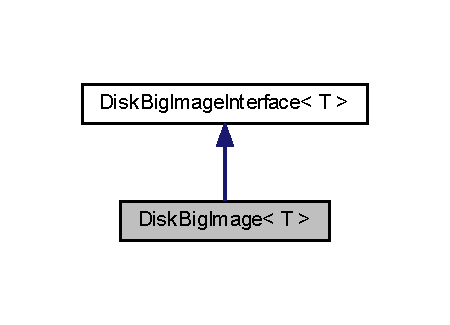
\includegraphics[width=216pt]{class_disk_big_image__inherit__graph}
\end{center}
\end{figure}


Disk\-Big\-Image$<$ T $>$ 的协作图\-:\nopagebreak
\begin{figure}[H]
\begin{center}
\leavevmode
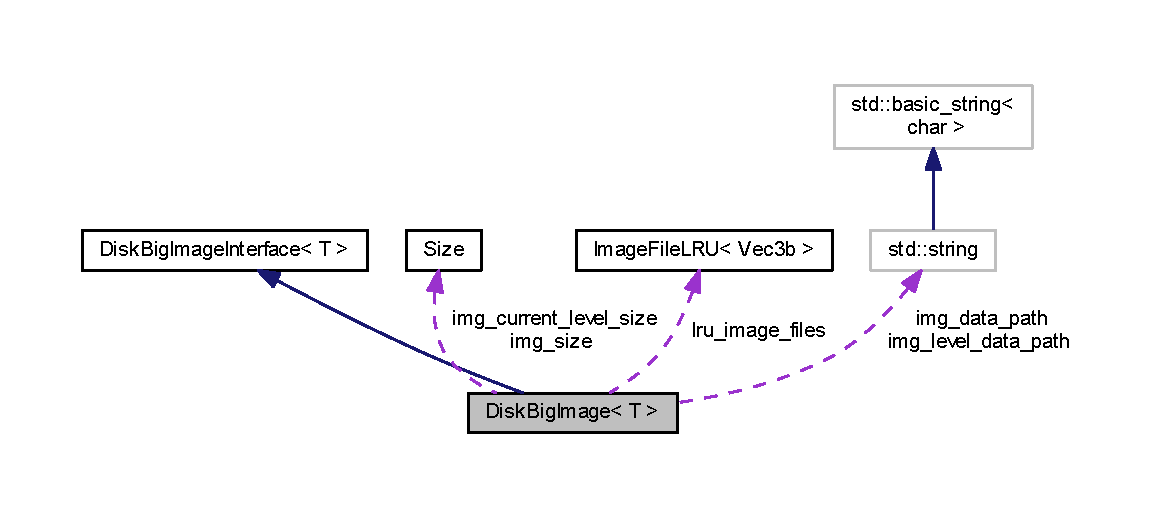
\includegraphics[width=350pt]{class_disk_big_image__coll__graph}
\end{center}
\end{figure}
\subsection*{类}
\begin{DoxyCompactItemize}
\item 
struct {\bf Data\-Index\-Info}
\begin{DoxyCompactList}\small\item\em This structure is used in the \doxyref{get\-\_\-pixels\-\_\-by\-\_\-level()}{p.}{class_disk_big_image_a9b8062ca60135249493571a6f47da1ef} function to sort the range data. \end{DoxyCompactList}\end{DoxyCompactItemize}
\subsection*{Public 成员函数}
\begin{DoxyCompactItemize}
\item 
virtual bool {\bf get\-\_\-pixels\-\_\-by\-\_\-level} (int level, int start\-\_\-row, int start\-\_\-col, int rows, int cols, std\-::vector$<$ T $>$ \&vec)
\begin{DoxyCompactList}\small\item\em Get the the specific range area image data from the bigimage files, but first specific which level data you want to get. \end{DoxyCompactList}\item 
virtual bool {\bfseries set\-\_\-pixel\-\_\-by\-\_\-level} (int level, int start\-\_\-row, int start\-\_\-col, int rows, int cols, const std\-::vector$<$ T $>$ \&vec)\label{class_disk_big_image_adb18569f0434d28df54056ba5a46128b}

\item 
virtual bool {\bfseries get\-\_\-pixels\-\_\-by\-\_\-level\-\_\-fast} (int level, int \&start\-\_\-row, int \&start\-\_\-col, int \&rows, int \&cols, std\-::vector$<$ T $>$ \&vec)\label{class_disk_big_image_a0f2ab14d3ee9d1b5214c95bf20c1559c}

\item 
virtual bool {\bf set\-\_\-current\-\_\-level} (int level)\label{class_disk_big_image_a721b35955145235b188b54e964b9df7c}

\begin{DoxyCompactList}\small\item\em set the image current level before any access to the hierarchical image data \end{DoxyCompactList}\item 
virtual size\-\_\-t {\bfseries get\-\_\-current\-\_\-level} () const \label{class_disk_big_image_ae2197d930170ed4cd012b43e74d0a487}

\item 
virtual size\-\_\-t {\bf get\-\_\-current\-\_\-level\-\_\-image\-\_\-rows} () const \label{class_disk_big_image_a0069752abef86aca7017c480fbd74f60}

\begin{DoxyCompactList}\small\item\em get the current level image rows after calling the set\-\_\-current\-\_\-level function \end{DoxyCompactList}\item 
virtual size\-\_\-t {\bf get\-\_\-current\-\_\-level\-\_\-image\-\_\-cols} () const \label{class_disk_big_image_a2a81a18bdf3fe321125b780f02c8d3ef}

\begin{DoxyCompactList}\small\item\em get the current level image cols after calling the set\-\_\-current\-\_\-level function \end{DoxyCompactList}\item 
virtual bool {\bf set\-\_\-file\-\_\-cache\-\_\-number} (int \-\_\-file\-\_\-cache\-\_\-number)\label{class_disk_big_image_a20d09cacae5a25b71c716563451c05aa}

\begin{DoxyCompactList}\small\item\em set the file cache number when loading image data since the image from disk is too large so when load data from disk, using several file caches to save the image data for improving I/\-O. \end{DoxyCompactList}\item 
virtual size\-\_\-t {\bf get\-\_\-max\-\_\-image\-\_\-level} () const \label{class_disk_big_image_a3d58d791486db6c65b56a46256ef2b36}

\begin{DoxyCompactList}\small\item\em get the maximum image level thus the minimal size image's scale level \end{DoxyCompactList}\item 
size\-\_\-t {\bf get\-\_\-minimal\-\_\-image\-\_\-rows} () const 
\begin{DoxyCompactList}\small\item\em get the minimal\-\_\-image size. \end{DoxyCompactList}\item 
size\-\_\-t {\bfseries get\-\_\-minimal\-\_\-image\-\_\-cols} () const \label{class_disk_big_image_a34d024eb203ee99749d9344ce81129ff}

\item 
size\-\_\-t {\bf get\-\_\-image\-\_\-rows} () const 
\begin{DoxyCompactList}\small\item\em get the total image size. \end{DoxyCompactList}\item 
size\-\_\-t {\bfseries get\-\_\-image\-\_\-cols} () const \label{class_disk_big_image_a95dfc7852db1866614a64b1edfa38e74}

\end{DoxyCompactItemize}
\subsection*{Protected 成员函数}
\begin{DoxyCompactItemize}
\item 
bool {\bf read\-\_\-from\-\_\-index\-\_\-range} (size\-\_\-t front, size\-\_\-t tail, {\bf Z\-Order\-Index\-::\-Index\-Type} start\-\_\-index, const std\-::vector$<$ {\bf Data\-Index\-Info} $>$ \&index\-\_\-info\-\_\-vector, std\-::vector$<$ T $>$ \&data\-\_\-vector)\label{class_disk_big_image_a23754f55994fd2e7761ad1c437a5642d}

\begin{DoxyCompactList}\small\item\em read out the [front, tail) range cells in the index\-\_\-info\-\_\-vector, write the data into the data\-\_\-vector, which keeps the row-\/major format image data that comes to be the result of \doxyref{get\-\_\-pixels\-\_\-by\-\_\-level()}{p.}{class_disk_big_image_a9b8062ca60135249493571a6f47da1ef} function. \end{DoxyCompactList}\item 
bool {\bf check\-\_\-para\-\_\-validation} (int level, int start\-\_\-row, int start\-\_\-col, int rows, int cols)\label{class_disk_big_image_a2c98bd73bd9046c5b24a0a10cf318eb7}

\begin{DoxyCompactList}\small\item\em checks the parameter invalidation before calling the \doxyref{get\-\_\-pixels\-\_\-by\-\_\-level()}{p.}{class_disk_big_image_a9b8062ca60135249493571a6f47da1ef} function \end{DoxyCompactList}\item 
bool {\bf load\-\_\-image\-\_\-head\-\_\-file} (const char $\ast$file\-\_\-name)\label{class_disk_big_image_a69e29d2fca837ffb8c453b0630a6b988}

\begin{DoxyCompactList}\small\item\em load the image head file before load image \end{DoxyCompactList}\item 
void {\bf set\-\_\-image\-\_\-data\-\_\-path} (const char $\ast$file\-\_\-name)\label{class_disk_big_image_a7edcce6b2059844d395ef86ae241eb31}

\begin{DoxyCompactList}\small\item\em get he image data path form the file\-\_\-name($\ast$.bigimage) \end{DoxyCompactList}\item 
{\bf Disk\-Big\-Image} ()
\begin{DoxyCompactList}\small\item\em \doxyref{Disk\-Big\-Image}{p.}{class_disk_big_image} can only be constructed in the subclass or friend function. Main used in the load\-\_\-disk\-\_\-image function to get a new object from the big image file. \end{DoxyCompactList}\end{DoxyCompactItemize}
\subsection*{Protected 属性}
\begin{DoxyCompactItemize}
\item 
{\bf Size} {\bf img\-\_\-size}
\item 
int64 {\bf file\-\_\-node\-\_\-size}
\item 
int64 {\bf file\-\_\-node\-\_\-shift\-\_\-num}
\item 
boost\-::shared\-\_\-ptr\\*
$<$ {\bf Index\-Method\-Interface} $>$ {\bf index\-\_\-method}
\item 
size\-\_\-t {\bf m\-\_\-mini\-\_\-rows}
\item 
size\-\_\-t {\bfseries m\-\_\-mini\-\_\-cols}\label{class_disk_big_image_af953d4d9f81bfb39ab537e94782889b9}

\item 
size\-\_\-t {\bf m\-\_\-max\-\_\-level}
\item 
{\bf Size} {\bf img\-\_\-current\-\_\-level\-\_\-size}
\item 
size\-\_\-t {\bf m\-\_\-current\-\_\-level}
\item 
std\-::string {\bf img\-\_\-data\-\_\-path}
\item 
std\-::string {\bf img\-\_\-level\-\_\-data\-\_\-path}
\item 
size\-\_\-t {\bf file\-\_\-cache\-\_\-number}
\item 
{\bf Image\-File\-L\-R\-U}$<$ {\bf Vec3b} $>$ {\bf lru\-\_\-image\-\_\-files}
\end{DoxyCompactItemize}
\subsection*{友元}
\begin{DoxyCompactItemize}
\item 
{\footnotesize template$<$typename T $>$ }\\boost\-::shared\-\_\-ptr\\*
$<$ {\bf Disk\-Big\-Image}$<$ T $>$ $>$ {\bf load\-\_\-disk\-\_\-image} (const char $\ast$file\-\_\-name)
\begin{DoxyCompactList}\small\item\em The main function to load a big image file from disk. \end{DoxyCompactList}\end{DoxyCompactItemize}


\subsection{详细描述}
\subsubsection*{template$<$typename T$>$class Disk\-Big\-Image$<$ T $>$}

Derived from \doxyref{Disk\-Big\-Image\-Interface}{p.}{class_disk_big_image_interface}, support for the reading and writing of the big image that was saved in the disk. 

The big image saved in the disk comes from the \doxyref{Blockwise\-Image}{p.}{class_blockwise_image} class or \doxyref{Hierarchical\-Image}{p.}{class_hierarchical_image} class. This class is used to access the image data in the disk at a low cost of using memory usage. When access the image data, the last frequently used image data will be save in the memory, and the none frequently used image data will be swap out to the disk.


\begin{DoxyTemplParams}{Template Parameters}
{\em T} & The type of the image cell \\
\hline
\end{DoxyTemplParams}
\begin{Desc}
\item[示例\-: ]\par
{\bf test\-Image\-Containter.\-cpp}.\end{Desc}


在文件 {\bf Disk\-Big\-Image.\-h} 第  行定义.



\subsection{构造及析构函数说明}
\index{Disk\-Big\-Image@{Disk\-Big\-Image}!Disk\-Big\-Image@{Disk\-Big\-Image}}
\index{Disk\-Big\-Image@{Disk\-Big\-Image}!DiskBigImage@{Disk\-Big\-Image}}
\subsubsection[{Disk\-Big\-Image}]{\setlength{\rightskip}{0pt plus 5cm}template$<$typename T $>$ {\bf Disk\-Big\-Image}$<$ T $>$\-::{\bf Disk\-Big\-Image} (
\begin{DoxyParamCaption}
{}
\end{DoxyParamCaption}
)\hspace{0.3cm}{\ttfamily [inline]}, {\ttfamily [protected]}}\label{class_disk_big_image_a9e922356e4dc2b5f8f15350b077a8bd3}


\doxyref{Disk\-Big\-Image}{p.}{class_disk_big_image} can only be constructed in the subclass or friend function. Main used in the load\-\_\-disk\-\_\-image function to get a new object from the big image file. 

\begin{DoxySeeAlso}{参见}
\doxyref{load\-\_\-disk\-\_\-image()}{p.}{class_disk_big_image_a290d5c0bf83af4cf17fe0b7eb1abd3bb} 
\end{DoxySeeAlso}


在文件 {\bf Disk\-Big\-Image.\-h} 第  行定义.



\subsection{成员函数说明}
\index{Disk\-Big\-Image@{Disk\-Big\-Image}!get\-\_\-image\-\_\-rows@{get\-\_\-image\-\_\-rows}}
\index{get\-\_\-image\-\_\-rows@{get\-\_\-image\-\_\-rows}!DiskBigImage@{Disk\-Big\-Image}}
\subsubsection[{get\-\_\-image\-\_\-rows}]{\setlength{\rightskip}{0pt plus 5cm}template$<$typename T $>$ size\-\_\-t {\bf Disk\-Big\-Image}$<$ T $>$\-::get\-\_\-image\-\_\-rows (
\begin{DoxyParamCaption}
{}
\end{DoxyParamCaption}
) const\hspace{0.3cm}{\ttfamily [inline]}}\label{class_disk_big_image_a068e610d1db01a4d8ee93a1cbab0c99d}


get the total image size. 

The size info can also be got by calling such functions. 1) set\-\_\-current\-\_\-level(0); 2) \doxyref{get\-\_\-current\-\_\-level\-\_\-image\-\_\-rows()}{p.}{class_disk_big_image_a0069752abef86aca7017c480fbd74f60} \&\& \doxyref{get\-\_\-current\-\_\-level\-\_\-image\-\_\-cols()}{p.}{class_disk_big_image_a2a81a18bdf3fe321125b780f02c8d3ef} 

在文件 {\bf Disk\-Big\-Image.\-h} 第  行定义.

\index{Disk\-Big\-Image@{Disk\-Big\-Image}!get\-\_\-minimal\-\_\-image\-\_\-rows@{get\-\_\-minimal\-\_\-image\-\_\-rows}}
\index{get\-\_\-minimal\-\_\-image\-\_\-rows@{get\-\_\-minimal\-\_\-image\-\_\-rows}!DiskBigImage@{Disk\-Big\-Image}}
\subsubsection[{get\-\_\-minimal\-\_\-image\-\_\-rows}]{\setlength{\rightskip}{0pt plus 5cm}template$<$typename T $>$ size\-\_\-t {\bf Disk\-Big\-Image}$<$ T $>$\-::get\-\_\-minimal\-\_\-image\-\_\-rows (
\begin{DoxyParamCaption}
{}
\end{DoxyParamCaption}
) const\hspace{0.3cm}{\ttfamily [inline]}}\label{class_disk_big_image_ad89988c077d526505993a82477ccdc13}


get the minimal\-\_\-image size. 

The size info can also be got by calling such functions. 1) set\-\_\-current\-\_\-level(\doxyref{get\-\_\-max\-\_\-image\-\_\-level()}{p.}{class_disk_big_image_a3d58d791486db6c65b56a46256ef2b36}); 2) \doxyref{get\-\_\-current\-\_\-level\-\_\-image\-\_\-rows()}{p.}{class_disk_big_image_a0069752abef86aca7017c480fbd74f60} \&\& \doxyref{get\-\_\-current\-\_\-level\-\_\-image\-\_\-cols()}{p.}{class_disk_big_image_a2a81a18bdf3fe321125b780f02c8d3ef} 

在文件 {\bf Disk\-Big\-Image.\-h} 第  行定义.

\index{Disk\-Big\-Image@{Disk\-Big\-Image}!get\-\_\-pixels\-\_\-by\-\_\-level@{get\-\_\-pixels\-\_\-by\-\_\-level}}
\index{get\-\_\-pixels\-\_\-by\-\_\-level@{get\-\_\-pixels\-\_\-by\-\_\-level}!DiskBigImage@{Disk\-Big\-Image}}
\subsubsection[{get\-\_\-pixels\-\_\-by\-\_\-level}]{\setlength{\rightskip}{0pt plus 5cm}template$<$typename T $>$ bool {\bf Disk\-Big\-Image}$<$ T $>$\-::get\-\_\-pixels\-\_\-by\-\_\-level (
\begin{DoxyParamCaption}
\item[{int}]{level, }
\item[{int}]{start\-\_\-row, }
\item[{int}]{start\-\_\-col, }
\item[{int}]{rows, }
\item[{int}]{cols, }
\item[{std\-::vector$<$ T $>$ \&}]{vec}
\end{DoxyParamCaption}
)\hspace{0.3cm}{\ttfamily [virtual]}}\label{class_disk_big_image_a9b8062ca60135249493571a6f47da1ef}


Get the the specific range area image data from the bigimage files, but first specific which level data you want to get. 


\begin{DoxyParams}{参数}
{\em level} & The specific level \\
\hline
{\em start\-\_\-row} & The left-\/corner point row \\
\hline
{\em start\-\_\-col} & The left-\/corner point col \\
\hline
{\em rows} & The row scope of the range, thus the rows get is [start\-\_\-row, start\-\_\-row + rows) \\
\hline
{\em cols} & The col scope of the range \\
\hline
{\em vec} & [Out] Saves the image data get from the bigimage files \\
\hline
\end{DoxyParams}
\begin{DoxyReturn}{返回}
whether get the data successfully 
\end{DoxyReturn}


实现了 {\bf Disk\-Big\-Image\-Interface$<$ T $>$} \doxyref{}{p.}{class_disk_big_image_interface_a1f9a1750bc7f2da534310958e89c64b5}.



在文件 {\bf Disk\-Big\-Image.\-hpp} 第  行定义.



\subsection{友元及相关函数文档}
\index{Disk\-Big\-Image@{Disk\-Big\-Image}!load\-\_\-disk\-\_\-image@{load\-\_\-disk\-\_\-image}}
\index{load\-\_\-disk\-\_\-image@{load\-\_\-disk\-\_\-image}!DiskBigImage@{Disk\-Big\-Image}}
\subsubsection[{load\-\_\-disk\-\_\-image}]{\setlength{\rightskip}{0pt plus 5cm}template$<$typename T $>$ template$<$typename T $>$ boost\-::shared\-\_\-ptr$<${\bf Disk\-Big\-Image}$<$T$>$ $>$ load\-\_\-disk\-\_\-image (
\begin{DoxyParamCaption}
\item[{const char $\ast$}]{file\-\_\-name}
\end{DoxyParamCaption}
)\hspace{0.3cm}{\ttfamily [friend]}}\label{class_disk_big_image_a290d5c0bf83af4cf17fe0b7eb1abd3bb}


The main function to load a big image file from disk. 

file\-\_\-name The file name of the big image header file (the extension is .bigimage) \begin{DoxyReturn}{返回}
the shared\-\_\-ptr of the big image object \doxyref{Disk\-Big\-Image}{p.}{class_disk_big_image} 
\end{DoxyReturn}


在文件 {\bf Disk\-Big\-Image.\-hpp} 第  行定义.



\subsection{类成员变量说明}
\index{Disk\-Big\-Image@{Disk\-Big\-Image}!file\-\_\-cache\-\_\-number@{file\-\_\-cache\-\_\-number}}
\index{file\-\_\-cache\-\_\-number@{file\-\_\-cache\-\_\-number}!DiskBigImage@{Disk\-Big\-Image}}
\subsubsection[{file\-\_\-cache\-\_\-number}]{\setlength{\rightskip}{0pt plus 5cm}template$<$typename T $>$ size\-\_\-t {\bf Disk\-Big\-Image}$<$ T $>$\-::file\-\_\-cache\-\_\-number\hspace{0.3cm}{\ttfamily [protected]}}\label{class_disk_big_image_a993a1b7f4a08dcff802e0895c4cc0d9d}
the number of cache file number for lru manager 

在文件 {\bf Disk\-Big\-Image.\-h} 第  行定义.

\index{Disk\-Big\-Image@{Disk\-Big\-Image}!file\-\_\-node\-\_\-shift\-\_\-num@{file\-\_\-node\-\_\-shift\-\_\-num}}
\index{file\-\_\-node\-\_\-shift\-\_\-num@{file\-\_\-node\-\_\-shift\-\_\-num}!DiskBigImage@{Disk\-Big\-Image}}
\subsubsection[{file\-\_\-node\-\_\-shift\-\_\-num}]{\setlength{\rightskip}{0pt plus 5cm}template$<$typename T $>$ int64 {\bf Disk\-Big\-Image}$<$ T $>$\-::file\-\_\-node\-\_\-shift\-\_\-num\hspace{0.3cm}{\ttfamily [protected]}}\label{class_disk_big_image_ab081b11ac1701d751c31a48388fd17d7}
the shift number of file\-\_\-node\-\_\-size 

在文件 {\bf Disk\-Big\-Image.\-h} 第  行定义.

\index{Disk\-Big\-Image@{Disk\-Big\-Image}!file\-\_\-node\-\_\-size@{file\-\_\-node\-\_\-size}}
\index{file\-\_\-node\-\_\-size@{file\-\_\-node\-\_\-size}!DiskBigImage@{Disk\-Big\-Image}}
\subsubsection[{file\-\_\-node\-\_\-size}]{\setlength{\rightskip}{0pt plus 5cm}template$<$typename T $>$ int64 {\bf Disk\-Big\-Image}$<$ T $>$\-::file\-\_\-node\-\_\-size\hspace{0.3cm}{\ttfamily [protected]}}\label{class_disk_big_image_a6cea55287b598387220c2de1372e8f1e}
the number of cells in individual file 

在文件 {\bf Disk\-Big\-Image.\-h} 第  行定义.

\index{Disk\-Big\-Image@{Disk\-Big\-Image}!img\-\_\-current\-\_\-level\-\_\-size@{img\-\_\-current\-\_\-level\-\_\-size}}
\index{img\-\_\-current\-\_\-level\-\_\-size@{img\-\_\-current\-\_\-level\-\_\-size}!DiskBigImage@{Disk\-Big\-Image}}
\subsubsection[{img\-\_\-current\-\_\-level\-\_\-size}]{\setlength{\rightskip}{0pt plus 5cm}template$<$typename T $>$ {\bf Size} {\bf Disk\-Big\-Image}$<$ T $>$\-::img\-\_\-current\-\_\-level\-\_\-size\hspace{0.3cm}{\ttfamily [protected]}}\label{class_disk_big_image_afdecdad1aa6fe0aef3532126a13c7bde}
the image current level 

在文件 {\bf Disk\-Big\-Image.\-h} 第  行定义.

\index{Disk\-Big\-Image@{Disk\-Big\-Image}!img\-\_\-data\-\_\-path@{img\-\_\-data\-\_\-path}}
\index{img\-\_\-data\-\_\-path@{img\-\_\-data\-\_\-path}!DiskBigImage@{Disk\-Big\-Image}}
\subsubsection[{img\-\_\-data\-\_\-path}]{\setlength{\rightskip}{0pt plus 5cm}template$<$typename T $>$ std\-::string {\bf Disk\-Big\-Image}$<$ T $>$\-::img\-\_\-data\-\_\-path\hspace{0.3cm}{\ttfamily [protected]}}\label{class_disk_big_image_a3b1f866ae3a06ac5a54372d714bd66de}
the path of the image data in filesystem 

在文件 {\bf Disk\-Big\-Image.\-h} 第  行定义.

\index{Disk\-Big\-Image@{Disk\-Big\-Image}!img\-\_\-level\-\_\-data\-\_\-path@{img\-\_\-level\-\_\-data\-\_\-path}}
\index{img\-\_\-level\-\_\-data\-\_\-path@{img\-\_\-level\-\_\-data\-\_\-path}!DiskBigImage@{Disk\-Big\-Image}}
\subsubsection[{img\-\_\-level\-\_\-data\-\_\-path}]{\setlength{\rightskip}{0pt plus 5cm}template$<$typename T $>$ std\-::string {\bf Disk\-Big\-Image}$<$ T $>$\-::img\-\_\-level\-\_\-data\-\_\-path\hspace{0.3cm}{\ttfamily [protected]}}\label{class_disk_big_image_a4cd979aed67cc7fe4cbd25ea8515426e}
the specific level image data path 

在文件 {\bf Disk\-Big\-Image.\-h} 第  行定义.

\index{Disk\-Big\-Image@{Disk\-Big\-Image}!img\-\_\-size@{img\-\_\-size}}
\index{img\-\_\-size@{img\-\_\-size}!DiskBigImage@{Disk\-Big\-Image}}
\subsubsection[{img\-\_\-size}]{\setlength{\rightskip}{0pt plus 5cm}template$<$typename T $>$ {\bf Size} {\bf Disk\-Big\-Image}$<$ T $>$\-::img\-\_\-size\hspace{0.3cm}{\ttfamily [protected]}}\label{class_disk_big_image_adbef855945a2d4bf0d3f191930f7bafe}
saves the whole size of the image 

在文件 {\bf Disk\-Big\-Image.\-h} 第  行定义.

\index{Disk\-Big\-Image@{Disk\-Big\-Image}!index\-\_\-method@{index\-\_\-method}}
\index{index\-\_\-method@{index\-\_\-method}!DiskBigImage@{Disk\-Big\-Image}}
\subsubsection[{index\-\_\-method}]{\setlength{\rightskip}{0pt plus 5cm}template$<$typename T $>$ boost\-::shared\-\_\-ptr$<${\bf Index\-Method\-Interface}$>$ {\bf Disk\-Big\-Image}$<$ T $>$\-::index\-\_\-method\hspace{0.3cm}{\ttfamily [protected]}}\label{class_disk_big_image_ab33f5cec593d48264ffd7ae50eb52c18}
the shared\-\_\-ptr of index method 

在文件 {\bf Disk\-Big\-Image.\-h} 第  行定义.

\index{Disk\-Big\-Image@{Disk\-Big\-Image}!lru\-\_\-image\-\_\-files@{lru\-\_\-image\-\_\-files}}
\index{lru\-\_\-image\-\_\-files@{lru\-\_\-image\-\_\-files}!DiskBigImage@{Disk\-Big\-Image}}
\subsubsection[{lru\-\_\-image\-\_\-files}]{\setlength{\rightskip}{0pt plus 5cm}template$<$typename T $>$ {\bf Image\-File\-L\-R\-U}$<${\bf Vec3b}$>$ {\bf Disk\-Big\-Image}$<$ T $>$\-::lru\-\_\-image\-\_\-files\hspace{0.3cm}{\ttfamily [protected]}}\label{class_disk_big_image_a67a35f40b6b24062385ef6ea78d74128}
the lru image files manager 

在文件 {\bf Disk\-Big\-Image.\-h} 第  行定义.

\index{Disk\-Big\-Image@{Disk\-Big\-Image}!m\-\_\-current\-\_\-level@{m\-\_\-current\-\_\-level}}
\index{m\-\_\-current\-\_\-level@{m\-\_\-current\-\_\-level}!DiskBigImage@{Disk\-Big\-Image}}
\subsubsection[{m\-\_\-current\-\_\-level}]{\setlength{\rightskip}{0pt plus 5cm}template$<$typename T $>$ size\-\_\-t {\bf Disk\-Big\-Image}$<$ T $>$\-::m\-\_\-current\-\_\-level\hspace{0.3cm}{\ttfamily [protected]}}\label{class_disk_big_image_aafa946f7ccf8e4fe4f874137c391a938}
the current level for reading and writing 

在文件 {\bf Disk\-Big\-Image.\-h} 第  行定义.

\index{Disk\-Big\-Image@{Disk\-Big\-Image}!m\-\_\-max\-\_\-level@{m\-\_\-max\-\_\-level}}
\index{m\-\_\-max\-\_\-level@{m\-\_\-max\-\_\-level}!DiskBigImage@{Disk\-Big\-Image}}
\subsubsection[{m\-\_\-max\-\_\-level}]{\setlength{\rightskip}{0pt plus 5cm}template$<$typename T $>$ size\-\_\-t {\bf Disk\-Big\-Image}$<$ T $>$\-::m\-\_\-max\-\_\-level\hspace{0.3cm}{\ttfamily [protected]}}\label{class_disk_big_image_ae415c0b60a45c251dc3914595c0fce2a}
the max image hierarchical level level = 0 \-: means no scale level = n \-: means scale 1/2$^\wedge$n of original image 

在文件 {\bf Disk\-Big\-Image.\-h} 第  行定义.

\index{Disk\-Big\-Image@{Disk\-Big\-Image}!m\-\_\-mini\-\_\-rows@{m\-\_\-mini\-\_\-rows}}
\index{m\-\_\-mini\-\_\-rows@{m\-\_\-mini\-\_\-rows}!DiskBigImage@{Disk\-Big\-Image}}
\subsubsection[{m\-\_\-mini\-\_\-rows}]{\setlength{\rightskip}{0pt plus 5cm}template$<$typename T $>$ size\-\_\-t {\bf Disk\-Big\-Image}$<$ T $>$\-::m\-\_\-mini\-\_\-rows\hspace{0.3cm}{\ttfamily [protected]}}\label{class_disk_big_image_ab90ffbe6abf10151593240f789922693}
size of the minimum size image 

在文件 {\bf Disk\-Big\-Image.\-h} 第  行定义.



该类的文档由以下文件生成\-:\begin{DoxyCompactItemize}
\item 
D\-:/\-Out\-\_\-\-Of\-\_\-\-Core\-\_\-\-Git/src/Disk\-Big\-Image.\-h\item 
D\-:/\-Out\-\_\-\-Of\-\_\-\-Core\-\_\-\-Git/src/Disk\-Big\-Image.\-hpp\end{DoxyCompactItemize}

\section{Disk\-Big\-Image\-Interface$<$ T $>$ 模板类 参考}
\label{class_disk_big_image_interface}\index{Disk\-Big\-Image\-Interface$<$ T $>$@{Disk\-Big\-Image\-Interface$<$ T $>$}}


The interface for accessing the big image files in the disk that were saved by \doxyref{Blockwise\-Image}{p.}{class_blockwise_image} and \doxyref{Hierarchical\-Image}{p.}{class_hierarchical_image} classes.  




{\ttfamily \#include $<$Disk\-Big\-Image\-Interface.\-h$>$}



类 Disk\-Big\-Image\-Interface$<$ T $>$ 继承关系图\-:\nopagebreak
\begin{figure}[H]
\begin{center}
\leavevmode
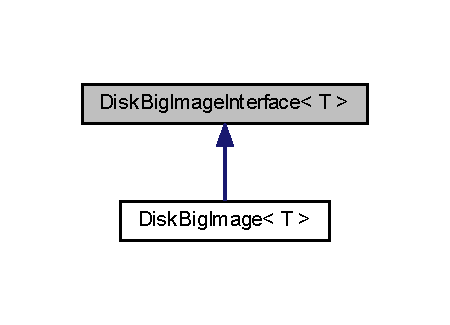
\includegraphics[width=216pt]{class_disk_big_image_interface__inherit__graph}
\end{center}
\end{figure}
\subsection*{Public 成员函数}
\begin{DoxyCompactItemize}
\item 
virtual bool {\bf get\-\_\-pixels\-\_\-by\-\_\-level} (int level, int start\-\_\-row, int start\-\_\-col, int rows, int cols, std\-::vector$<$ T $>$ \&vec)=0
\begin{DoxyCompactList}\small\item\em Get the the specific range area image data from the bigimage files, but first specific which level data you want to get. \end{DoxyCompactList}\item 
virtual bool {\bfseries set\-\_\-pixel\-\_\-by\-\_\-level} (int level, int start\-\_\-row, int start\-\_\-col, int rows, int cols, const std\-::vector$<$ T $>$ \&vec)=0\label{class_disk_big_image_interface_a8b119a9f7e1a73bb70f972e611579bec}

\item 
virtual bool {\bfseries get\-\_\-pixels\-\_\-by\-\_\-level\-\_\-fast} (int level, int \&start\-\_\-row, int \&start\-\_\-col, int \&rows, int \&cols, std\-::vector$<$ T $>$ \&vec)=0\label{class_disk_big_image_interface_a5ae50afa549df2025b0c0e8f2d9068cc}

\item 
virtual size\-\_\-t {\bf get\-\_\-current\-\_\-level\-\_\-image\-\_\-rows} () const =0\label{class_disk_big_image_interface_a908a572de60515e185b73d31baa5c48a}

\begin{DoxyCompactList}\small\item\em get the current level image rows after calling the set\-\_\-current\-\_\-level function \end{DoxyCompactList}\item 
virtual size\-\_\-t {\bf get\-\_\-current\-\_\-level\-\_\-image\-\_\-cols} () const =0\label{class_disk_big_image_interface_a05575b463c8d540eae947a70a1fa4101}

\begin{DoxyCompactList}\small\item\em get the current level image cols after calling the set\-\_\-current\-\_\-level function \end{DoxyCompactList}\item 
virtual bool {\bf set\-\_\-current\-\_\-level} (int level)=0\label{class_disk_big_image_interface_a81f77d04f54038b375fc4a9966db2223}

\begin{DoxyCompactList}\small\item\em set the image current level before any access to the hierarchical image data \end{DoxyCompactList}\item 
virtual size\-\_\-t {\bfseries get\-\_\-current\-\_\-level} () const =0\label{class_disk_big_image_interface_ac9c4da53d9e1d3b252bd48b4ba09516e}

\item 
virtual bool {\bf set\-\_\-file\-\_\-cache\-\_\-number} (int \-\_\-file\-\_\-cache\-\_\-number)=0\label{class_disk_big_image_interface_a56acf6b10340ce229a47044947409966}

\begin{DoxyCompactList}\small\item\em set the file cache number when loading image data since the image from disk is too large so when load data from disk, using several file caches to save the image data for improving I/\-O. \end{DoxyCompactList}\item 
virtual size\-\_\-t {\bf get\-\_\-max\-\_\-image\-\_\-level} () const =0\label{class_disk_big_image_interface_a120ee4945cf3fc38c21dad526128afc5}

\begin{DoxyCompactList}\small\item\em get the maximum image level thus the minimal size image's scale level \end{DoxyCompactList}\end{DoxyCompactItemize}


\subsection{详细描述}
\subsubsection*{template$<$typename T$>$class Disk\-Big\-Image\-Interface$<$ T $>$}

The interface for accessing the big image files in the disk that were saved by \doxyref{Blockwise\-Image}{p.}{class_blockwise_image} and \doxyref{Hierarchical\-Image}{p.}{class_hierarchical_image} classes. 


\begin{DoxyTemplParams}{Template Parameters}
{\em T} & The type of the image cells \\
\hline
\end{DoxyTemplParams}


在文件 {\bf Disk\-Big\-Image\-Interface.\-h} 第  行定义.



\subsection{成员函数说明}
\index{Disk\-Big\-Image\-Interface@{Disk\-Big\-Image\-Interface}!get\-\_\-pixels\-\_\-by\-\_\-level@{get\-\_\-pixels\-\_\-by\-\_\-level}}
\index{get\-\_\-pixels\-\_\-by\-\_\-level@{get\-\_\-pixels\-\_\-by\-\_\-level}!DiskBigImageInterface@{Disk\-Big\-Image\-Interface}}
\subsubsection[{get\-\_\-pixels\-\_\-by\-\_\-level}]{\setlength{\rightskip}{0pt plus 5cm}template$<$typename T $>$ virtual bool {\bf Disk\-Big\-Image\-Interface}$<$ T $>$\-::get\-\_\-pixels\-\_\-by\-\_\-level (
\begin{DoxyParamCaption}
\item[{int}]{level, }
\item[{int}]{start\-\_\-row, }
\item[{int}]{start\-\_\-col, }
\item[{int}]{rows, }
\item[{int}]{cols, }
\item[{std\-::vector$<$ T $>$ \&}]{vec}
\end{DoxyParamCaption}
)\hspace{0.3cm}{\ttfamily [pure virtual]}}\label{class_disk_big_image_interface_a1f9a1750bc7f2da534310958e89c64b5}


Get the the specific range area image data from the bigimage files, but first specific which level data you want to get. 


\begin{DoxyParams}{参数}
{\em level} & The specific level \\
\hline
{\em start\-\_\-row} & The left-\/corner point row \\
\hline
{\em start\-\_\-col} & The left-\/corner point col \\
\hline
{\em rows} & The row scope of the range, thus the rows get is [start\-\_\-row, start\-\_\-row + rows) \\
\hline
{\em cols} & The col scope of the range \\
\hline
{\em vec} & [Out] Saves the image data get from the bigimage files \\
\hline
\end{DoxyParams}
\begin{DoxyReturn}{返回}
whether get the data successfully 
\end{DoxyReturn}


在 {\bf Disk\-Big\-Image$<$ T $>$} \doxyref{}{p.}{class_disk_big_image_a9b8062ca60135249493571a6f47da1ef} 内被实现.



该类的文档由以下文件生成\-:\begin{DoxyCompactItemize}
\item 
D\-:/\-Out\-\_\-\-Of\-\_\-\-Core\-\_\-\-Git/src/Disk\-Big\-Image\-Interface.\-h\end{DoxyCompactItemize}

\section{Giant\-Image\-Interface$<$ T $>$ 模板类 参考}
\label{class_giant_image_interface}\index{Giant\-Image\-Interface$<$ T $>$@{Giant\-Image\-Interface$<$ T $>$}}


Derived form the \doxyref{Image\-Interface}{p.}{class_image_interface}, and defines the basic operations that restricted to the big image file accessing and operation.  




{\ttfamily \#include $<$Giant\-Image\-Interface.\-h$>$}



类 Giant\-Image\-Interface$<$ T $>$ 继承关系图\-:\nopagebreak
\begin{figure}[H]
\begin{center}
\leavevmode
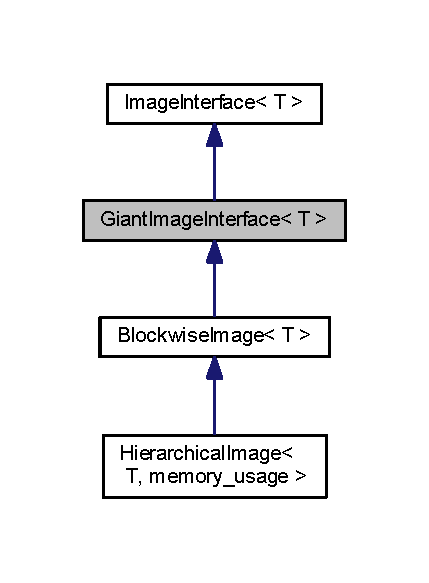
\includegraphics[width=206pt]{class_giant_image_interface__inherit__graph}
\end{center}
\end{figure}


Giant\-Image\-Interface$<$ T $>$ 的协作图\-:\nopagebreak
\begin{figure}[H]
\begin{center}
\leavevmode
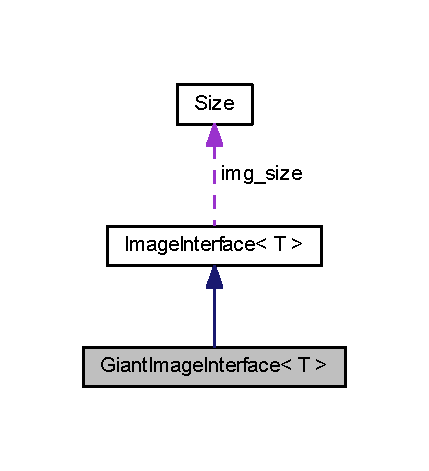
\includegraphics[width=206pt]{class_giant_image_interface__coll__graph}
\end{center}
\end{figure}
\subsection*{Public 成员函数}
\begin{DoxyCompactItemize}
\item 
{\bf Giant\-Image\-Interface} (boost\-::shared\-\_\-ptr$<$ {\bf Index\-Method\-Interface} $>$ method)
\item 
void {\bf set\-\_\-file\-\_\-node\-\_\-size} (int64 size)
\begin{DoxyCompactList}\small\item\em Set the size of each image data file (big image will be saved as many small image data files) \end{DoxyCompactList}\item 
int64 {\bfseries get\-\_\-file\-\_\-node\-\_\-size} () const \label{class_giant_image_interface_ada6eb717c2769231d4afad89eb5543a9}

\item 
void {\bf set\-\_\-index\-\_\-method} (boost\-::shared\-\_\-ptr$<$ {\bf Index\-Method\-Interface} $>$ method)
\begin{DoxyCompactList}\small\item\em set the new index object for internal indexing \end{DoxyCompactList}\item 
boost\-::shared\-\_\-ptr\\*
$<$ {\bf Index\-Method\-Interface} $>$ {\bfseries get\-\_\-index\-\_\-method} () const \label{class_giant_image_interface_a0a024409687eab4e31914a4f97a57d94}

\item 
virtual T \& {\bf at} ({\bf Index\-Method\-Interface\-::\-Index\-Type} index)=0
\begin{DoxyCompactList}\small\item\em get the element by the one dimension index \end{DoxyCompactList}\item 
virtual const T \& {\bfseries at} ({\bf Index\-Method\-Interface\-::\-Index\-Type} index) const =0\label{class_giant_image_interface_ab2416bbaab4b0cb63668d9d196b8a474}

\end{DoxyCompactItemize}
\subsection*{Protected 属性}
\begin{DoxyCompactItemize}
\item 
int64 {\bf file\-\_\-node\-\_\-size}
\item 
int64 {\bf file\-\_\-node\-\_\-shift\-\_\-num}
\item 
boost\-::shared\-\_\-ptr\\*
$<$ {\bf Index\-Method\-Interface} $>$ {\bf index\-\_\-method}
\end{DoxyCompactItemize}


\subsection{详细描述}
\subsubsection*{template$<$typename T$>$class Giant\-Image\-Interface$<$ T $>$}

Derived form the \doxyref{Image\-Interface}{p.}{class_image_interface}, and defines the basic operations that restricted to the big image file accessing and operation. 


\begin{DoxyTemplParams}{Template Parameters}
{\em The} & type of image cell \\
\hline
\end{DoxyTemplParams}
\begin{Desc}
\item[示例\-: ]\par
{\bf test\-Image\-Containter.\-cpp}.\end{Desc}


在文件 {\bf Giant\-Image\-Interface.\-h} 第  行定义.



\subsection{构造及析构函数说明}
\index{Giant\-Image\-Interface@{Giant\-Image\-Interface}!Giant\-Image\-Interface@{Giant\-Image\-Interface}}
\index{Giant\-Image\-Interface@{Giant\-Image\-Interface}!GiantImageInterface@{Giant\-Image\-Interface}}
\subsubsection[{Giant\-Image\-Interface}]{\setlength{\rightskip}{0pt plus 5cm}template$<$typename T $>$ {\bf Giant\-Image\-Interface}$<$ T $>$\-::{\bf Giant\-Image\-Interface} (
\begin{DoxyParamCaption}
\item[{boost\-::shared\-\_\-ptr$<$ {\bf Index\-Method\-Interface} $>$}]{method}
\end{DoxyParamCaption}
)\hspace{0.3cm}{\ttfamily [inline]}}\label{class_giant_image_interface_a29020cb121269a5343b1496f05cfc7b1}

\begin{DoxyParams}{参数}
{\em method} & the index method object for internal indexing \\
\hline
\end{DoxyParams}


在文件 {\bf Giant\-Image\-Interface.\-h} 第  行定义.



\subsection{成员函数说明}
\index{Giant\-Image\-Interface@{Giant\-Image\-Interface}!at@{at}}
\index{at@{at}!GiantImageInterface@{Giant\-Image\-Interface}}
\subsubsection[{at}]{\setlength{\rightskip}{0pt plus 5cm}template$<$typename T $>$ virtual T\& {\bf Giant\-Image\-Interface}$<$ T $>$\-::at (
\begin{DoxyParamCaption}
\item[{{\bf Index\-Method\-Interface\-::\-Index\-Type}}]{index}
\end{DoxyParamCaption}
)\hspace{0.3cm}{\ttfamily [pure virtual]}}\label{class_giant_image_interface_a1f98aece25249d626e60ebb9b0f05111}


get the element by the one dimension index 


\begin{DoxyParams}{参数}
{\em index} & one dimension index \\
\hline
\end{DoxyParams}


在 {\bf Blockwise\-Image$<$ T, memory\-\_\-usage $>$} \doxyref{}{p.}{class_blockwise_image_ab0cf952a4b988f8735dc770d9b0c787b} 内被实现.

\index{Giant\-Image\-Interface@{Giant\-Image\-Interface}!set\-\_\-file\-\_\-node\-\_\-size@{set\-\_\-file\-\_\-node\-\_\-size}}
\index{set\-\_\-file\-\_\-node\-\_\-size@{set\-\_\-file\-\_\-node\-\_\-size}!GiantImageInterface@{Giant\-Image\-Interface}}
\subsubsection[{set\-\_\-file\-\_\-node\-\_\-size}]{\setlength{\rightskip}{0pt plus 5cm}template$<$typename T $>$ void {\bf Giant\-Image\-Interface}$<$ T $>$\-::set\-\_\-file\-\_\-node\-\_\-size (
\begin{DoxyParamCaption}
\item[{int64}]{size}
\end{DoxyParamCaption}
)\hspace{0.3cm}{\ttfamily [inline]}}\label{class_giant_image_interface_aaa0c4aa9132cf27baa0d2ca5c22106f2}


Set the size of each image data file (big image will be saved as many small image data files) 


\begin{DoxyParams}{参数}
{\em size} & The file size in unit of byte \\
\hline
\end{DoxyParams}
make size the multiple of image cell's type

shift number \-: size == 2$^\wedge$(file\-\_\-node\-\_\-shift\-\_\-num) 

在文件 {\bf Giant\-Image\-Interface.\-h} 第  行定义.

\index{Giant\-Image\-Interface@{Giant\-Image\-Interface}!set\-\_\-index\-\_\-method@{set\-\_\-index\-\_\-method}}
\index{set\-\_\-index\-\_\-method@{set\-\_\-index\-\_\-method}!GiantImageInterface@{Giant\-Image\-Interface}}
\subsubsection[{set\-\_\-index\-\_\-method}]{\setlength{\rightskip}{0pt plus 5cm}template$<$typename T $>$ void {\bf Giant\-Image\-Interface}$<$ T $>$\-::set\-\_\-index\-\_\-method (
\begin{DoxyParamCaption}
\item[{boost\-::shared\-\_\-ptr$<$ {\bf Index\-Method\-Interface} $>$}]{method}
\end{DoxyParamCaption}
)\hspace{0.3cm}{\ttfamily [inline]}}\label{class_giant_image_interface_a64053aab159fe5bcdd6f9c4edf398bc4}


set the new index object for internal indexing 


\begin{DoxyParams}{参数}
{\em method} & the index object \\
\hline
\end{DoxyParams}


在文件 {\bf Giant\-Image\-Interface.\-h} 第  行定义.



\subsection{类成员变量说明}
\index{Giant\-Image\-Interface@{Giant\-Image\-Interface}!file\-\_\-node\-\_\-shift\-\_\-num@{file\-\_\-node\-\_\-shift\-\_\-num}}
\index{file\-\_\-node\-\_\-shift\-\_\-num@{file\-\_\-node\-\_\-shift\-\_\-num}!GiantImageInterface@{Giant\-Image\-Interface}}
\subsubsection[{file\-\_\-node\-\_\-shift\-\_\-num}]{\setlength{\rightskip}{0pt plus 5cm}template$<$typename T $>$ int64 {\bf Giant\-Image\-Interface}$<$ T $>$\-::file\-\_\-node\-\_\-shift\-\_\-num\hspace{0.3cm}{\ttfamily [protected]}}\label{class_giant_image_interface_a02542feca74e68b63faec27dea6f6495}
the shift number of file\-\_\-node\-\_\-size 

在文件 {\bf Giant\-Image\-Interface.\-h} 第  行定义.

\index{Giant\-Image\-Interface@{Giant\-Image\-Interface}!file\-\_\-node\-\_\-size@{file\-\_\-node\-\_\-size}}
\index{file\-\_\-node\-\_\-size@{file\-\_\-node\-\_\-size}!GiantImageInterface@{Giant\-Image\-Interface}}
\subsubsection[{file\-\_\-node\-\_\-size}]{\setlength{\rightskip}{0pt plus 5cm}template$<$typename T $>$ int64 {\bf Giant\-Image\-Interface}$<$ T $>$\-::file\-\_\-node\-\_\-size\hspace{0.3cm}{\ttfamily [protected]}}\label{class_giant_image_interface_a6e5f77de8944d9cf12220ae56af530fd}
the number of cells in individual file 

在文件 {\bf Giant\-Image\-Interface.\-h} 第  行定义.

\index{Giant\-Image\-Interface@{Giant\-Image\-Interface}!index\-\_\-method@{index\-\_\-method}}
\index{index\-\_\-method@{index\-\_\-method}!GiantImageInterface@{Giant\-Image\-Interface}}
\subsubsection[{index\-\_\-method}]{\setlength{\rightskip}{0pt plus 5cm}template$<$typename T $>$ boost\-::shared\-\_\-ptr$<${\bf Index\-Method\-Interface}$>$ {\bf Giant\-Image\-Interface}$<$ T $>$\-::index\-\_\-method\hspace{0.3cm}{\ttfamily [protected]}}\label{class_giant_image_interface_a42a95ed630071f83b0e67756d3b759f5}
the shared\-\_\-ptr of index method 

在文件 {\bf Giant\-Image\-Interface.\-h} 第  行定义.



该类的文档由以下文件生成\-:\begin{DoxyCompactItemize}
\item 
D\-:/\-Out\-\_\-\-Of\-\_\-\-Core\-\_\-\-Git/src/Giant\-Image\-Interface.\-h\end{DoxyCompactItemize}

\section{Hierarchical\-Image$<$ T, memory\-\_\-usage $>$ 模板类 参考}
\label{class_hierarchical_image}\index{Hierarchical\-Image$<$ T, memory\-\_\-usage $>$@{Hierarchical\-Image$<$ T, memory\-\_\-usage $>$}}


Derived from \doxyref{Blockwise\-Image}{p.}{class_blockwise_image}, support the big image operation, can save the image data in a hierarchical way.  




{\ttfamily \#include $<$Hierarchical\-Image.\-h$>$}



类 Hierarchical\-Image$<$ T, memory\-\_\-usage $>$ 继承关系图\-:\nopagebreak
\begin{figure}[H]
\begin{center}
\leavevmode
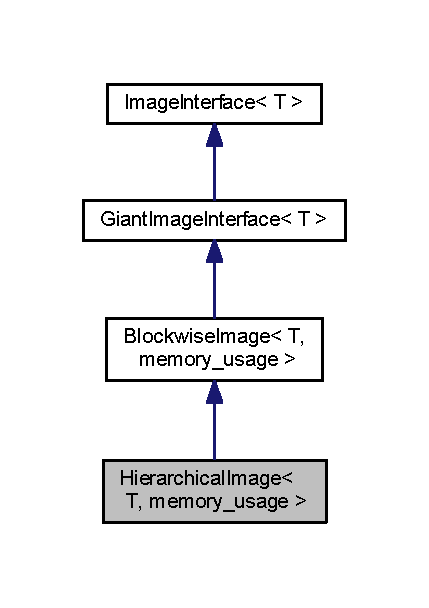
\includegraphics[width=206pt]{class_hierarchical_image__inherit__graph}
\end{center}
\end{figure}


Hierarchical\-Image$<$ T, memory\-\_\-usage $>$ 的协作图\-:\nopagebreak
\begin{figure}[H]
\begin{center}
\leavevmode
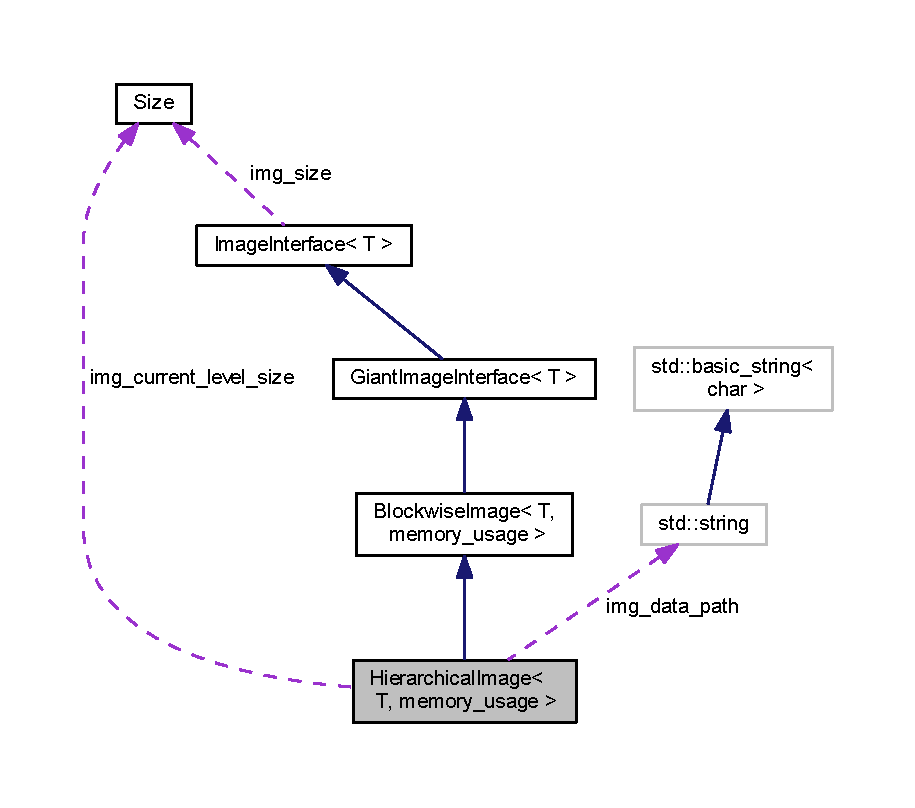
\includegraphics[width=350pt]{class_hierarchical_image__coll__graph}
\end{center}
\end{figure}
\subsection*{Public 成员函数}
\begin{DoxyCompactItemize}
\item 
{\bf Hierarchical\-Image} (size\-\_\-t rows, size\-\_\-t cols, size\-\_\-t mini\-\_\-rows, size\-\_\-t mini\-\_\-cols, boost\-::shared\-\_\-ptr$<$ {\bf Index\-Method\-Interface} $>$ method=boost\-::shared\-\_\-ptr$<$ {\bf Index\-Method\-Interface} $>$())
\item 
virtual bool {\bf write\-\_\-image} (const char $\ast$file\-\_\-name)
\item 
virtual bool {\bfseries write\-\_\-image} (const std\-::string \&file\-\_\-name)\label{class_hierarchical_image_a983ac78f154c2459eae807a740c5a4f2}

\item 
virtual bool {\bf save\-\_\-mini\-\_\-image} (const char $\ast$file\-\_\-name)
\begin{DoxyCompactList}\small\item\em save the mini size image as a jpg file for observation \end{DoxyCompactList}\item 
void {\bf set\-\_\-mutliply\-\_\-ways\-\_\-writing\-\_\-number} (size\-\_\-t number)
\begin{DoxyCompactList}\small\item\em set the number for writing image files concurrently \end{DoxyCompactList}\end{DoxyCompactItemize}
\subsection*{Protected 成员函数}
\begin{DoxyCompactItemize}
\item 
void {\bf set\-\_\-image\-\_\-data\-\_\-path} (const char $\ast$file\-\_\-name)
\begin{DoxyCompactList}\small\item\em set the image data path from the big image file name. \end{DoxyCompactList}\item 
bool {\bf write\-\_\-image\-\_\-head\-\_\-file} (const char $\ast$file\-\_\-name)\label{class_hierarchical_image_a4b34e191a90baabf547bc899a2822b0d}

\begin{DoxyCompactList}\small\item\em write the image head file \end{DoxyCompactList}\item 
bool {\bf write\-\_\-image\-\_\-inner\-\_\-loop} (size\-\_\-t start\-\_\-level, size\-\_\-t merge\-\_\-number, const boost\-::filesystem3\-::path \&data\-\_\-path, const int64 \&file\-\_\-number)\label{class_hierarchical_image_a2c2c982991f2f28cbf54f15266f507e5}

\begin{DoxyCompactList}\small\item\em write the start\-\_\-level image data in the write image inner loop \end{DoxyCompactList}\end{DoxyCompactItemize}
\subsection*{Protected 属性}
\begin{DoxyCompactItemize}
\item 
size\-\_\-t {\bf concurrent\-\_\-number}
\item 
std\-::string {\bf img\-\_\-data\-\_\-path}
\item 
{\bf Size} {\bf img\-\_\-current\-\_\-level\-\_\-size}
\end{DoxyCompactItemize}
\subsection*{相关函数}
(请注意\-: 这些不是成员函数.) \begin{DoxyCompactItemize}
\item 
{\footnotesize template$<$typename T $>$ }\\boost\-::shared\-\_\-ptr\\*
$<$ {\bf Giant\-Image\-Interface}$<$ T $>$ $>$ {\bf get\-\_\-hierarchical\-\_\-image\-\_\-by\-\_\-meomory\-\_\-usage} (unsigned memory\-\_\-usage, size\-\_\-t rows, size\-\_\-t cols, size\-\_\-t mini\-\_\-rows, size\-\_\-t mini\-\_\-cols, boost\-::shared\-\_\-ptr$<$ {\bf Index\-Method\-Interface} $>$ method=boost\-::shared\-\_\-ptr$<$ {\bf Index\-Method\-Interface} $>$())
\begin{DoxyCompactList}\small\item\em return the hierarchical image by memroy\-\_\-usage, maximum support 4\-G \end{DoxyCompactList}\end{DoxyCompactItemize}
\subsection*{额外继承的成员函数}


\subsection{详细描述}
\subsubsection*{template$<$typename T, size\-\_\-t memory\-\_\-usage = 64$>$class Hierarchical\-Image$<$ T, memory\-\_\-usage $>$}

Derived from \doxyref{Blockwise\-Image}{p.}{class_blockwise_image}, support the big image operation, can save the image data in a hierarchical way. 

\doxyref{Hierarchical\-Image}{p.}{class_hierarchical_image} can support very big image processing and storing, different with the \doxyref{Blockwise\-Image}{p.}{class_blockwise_image}, \doxyref{Hierarchical\-Image}{p.}{class_hierarchical_image} can write the image into different levels, but the \doxyref{Blockwise\-Image}{p.}{class_blockwise_image} can only save the full size of the image.


\begin{DoxyTemplParams}{Template Parameters}
{\em T} & The type of the image cell \\
\hline
{\em memory\-\_\-usage} & The memory usage used as a I/\-O cache in the main memory, and it must be bigger than 8 (in the unit of M). By default, memory\-\_\-usage is set to 64\-M \\
\hline
\end{DoxyTemplParams}
\begin{Desc}
\item[示例\-: ]\par
{\bf Write\-Hierarchical\-Image.\-cpp}.\end{Desc}


在文件 {\bf Hierarchical\-Image.\-h} 第  行定义.



\subsection{构造及析构函数说明}
\index{Hierarchical\-Image@{Hierarchical\-Image}!Hierarchical\-Image@{Hierarchical\-Image}}
\index{Hierarchical\-Image@{Hierarchical\-Image}!HierarchicalImage@{Hierarchical\-Image}}
\subsubsection[{Hierarchical\-Image}]{\setlength{\rightskip}{0pt plus 5cm}template$<$typename T , size\-\_\-t memory\-\_\-usage$>$ {\bf Hierarchical\-Image}$<$ T, memory\-\_\-usage $>$\-::{\bf Hierarchical\-Image} (
\begin{DoxyParamCaption}
\item[{size\-\_\-t}]{rows, }
\item[{size\-\_\-t}]{cols, }
\item[{size\-\_\-t}]{mini\-\_\-rows, }
\item[{size\-\_\-t}]{mini\-\_\-cols, }
\item[{boost\-::shared\-\_\-ptr$<$ {\bf Index\-Method\-Interface} $>$}]{method = {\ttfamily boost\-:\-:shared\-\_\-ptr$<${\bf Index\-Method\-Interface}$>$()}}
\end{DoxyParamCaption}
)}\label{class_hierarchical_image_a10037544868f5d2efc66993f8ddc23b0}

\begin{DoxyParams}{参数}
{\em rows} & the image total rows \\
\hline
{\em cols} & the image total cols \\
\hline
{\em mini\-\_\-rows} & the minimum size image rows \\
\hline
{\em mini\-\_\-cols} & the minimum size image cols \\
\hline
{\em method} & \-: the index method shared\-\_\-ptr object(default is zorder index method) \\
\hline
\end{DoxyParams}


在文件 {\bf Hierarchical\-Image.\-hpp} 第  行定义.



函数调用图\-:\nopagebreak
\begin{figure}[H]
\begin{center}
\leavevmode
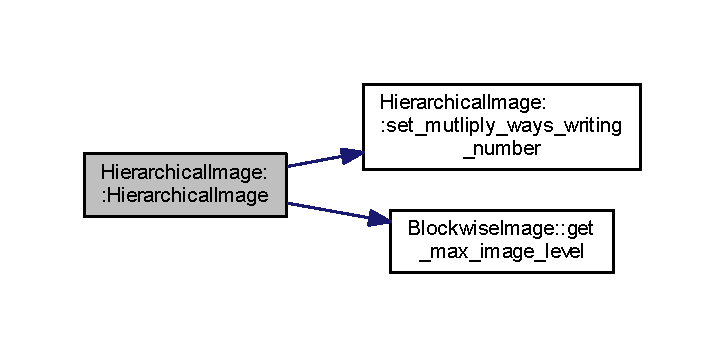
\includegraphics[width=348pt]{class_hierarchical_image_a10037544868f5d2efc66993f8ddc23b0_cgraph}
\end{center}
\end{figure}




\subsection{成员函数说明}
\index{Hierarchical\-Image@{Hierarchical\-Image}!save\-\_\-mini\-\_\-image@{save\-\_\-mini\-\_\-image}}
\index{save\-\_\-mini\-\_\-image@{save\-\_\-mini\-\_\-image}!HierarchicalImage@{Hierarchical\-Image}}
\subsubsection[{save\-\_\-mini\-\_\-image}]{\setlength{\rightskip}{0pt plus 5cm}template$<$typename T , size\-\_\-t memory\-\_\-usage$>$ bool {\bf Hierarchical\-Image}$<$ T, memory\-\_\-usage $>$\-::save\-\_\-mini\-\_\-image (
\begin{DoxyParamCaption}
\item[{const char $\ast$}]{file\-\_\-name}
\end{DoxyParamCaption}
)\hspace{0.3cm}{\ttfamily [virtual]}}\label{class_hierarchical_image_ad4c49535e55585ed7726856d8c65ef6e}


save the mini size image as a jpg file for observation 


\begin{DoxyParams}{参数}
{\em file\-\_\-name} & the bigimage file name ($\ast$.bigimage) \\
\hline
\end{DoxyParams}
\begin{DoxyNote}{注解}
if not defined the S\-A\-V\-E\-\_\-\-M\-I\-N\-I\-\_\-\-I\-M\-A\-G\-E macro, this function will do nothing 
\end{DoxyNote}


重载 {\bf Blockwise\-Image$<$ T, memory\-\_\-usage $>$} \doxyref{}{p.}{class_blockwise_image_a47ca8a383348f9cc527365977e9d721b} .



在文件 {\bf Hierarchical\-Image.\-hpp} 第  行定义.

\index{Hierarchical\-Image@{Hierarchical\-Image}!set\-\_\-image\-\_\-data\-\_\-path@{set\-\_\-image\-\_\-data\-\_\-path}}
\index{set\-\_\-image\-\_\-data\-\_\-path@{set\-\_\-image\-\_\-data\-\_\-path}!HierarchicalImage@{Hierarchical\-Image}}
\subsubsection[{set\-\_\-image\-\_\-data\-\_\-path}]{\setlength{\rightskip}{0pt plus 5cm}template$<$typename T , size\-\_\-t memory\-\_\-usage$>$ void {\bf Hierarchical\-Image}$<$ T, memory\-\_\-usage $>$\-::set\-\_\-image\-\_\-data\-\_\-path (
\begin{DoxyParamCaption}
\item[{const char $\ast$}]{file\-\_\-name}
\end{DoxyParamCaption}
)\hspace{0.3cm}{\ttfamily [inline]}, {\ttfamily [protected]}}\label{class_hierarchical_image_ae827b72365d1e8b65af0bf5c10a197d0}


set the image data path from the big image file name. 

For example \-: the file\-\_\-name is /a/x.bigimage then the data\-\_\-path is /a/x/ 

在文件 {\bf Hierarchical\-Image.\-h} 第  行定义.

\index{Hierarchical\-Image@{Hierarchical\-Image}!set\-\_\-mutliply\-\_\-ways\-\_\-writing\-\_\-number@{set\-\_\-mutliply\-\_\-ways\-\_\-writing\-\_\-number}}
\index{set\-\_\-mutliply\-\_\-ways\-\_\-writing\-\_\-number@{set\-\_\-mutliply\-\_\-ways\-\_\-writing\-\_\-number}!HierarchicalImage@{Hierarchical\-Image}}
\subsubsection[{set\-\_\-mutliply\-\_\-ways\-\_\-writing\-\_\-number}]{\setlength{\rightskip}{0pt plus 5cm}template$<$typename T , size\-\_\-t memory\-\_\-usage$>$ void {\bf Hierarchical\-Image}$<$ T, memory\-\_\-usage $>$\-::set\-\_\-mutliply\-\_\-ways\-\_\-writing\-\_\-number (
\begin{DoxyParamCaption}
\item[{size\-\_\-t}]{number}
\end{DoxyParamCaption}
)\hspace{0.3cm}{\ttfamily [inline]}}\label{class_hierarchical_image_a2f5b6691db32f8af8fff11a4982e88b9}


set the number for writing image files concurrently 

If the image has n levels(thus max level is n-\/1), then when write the image data in a hierarchical way into disk the maximum concurrent number is n. 

在文件 {\bf Hierarchical\-Image.\-h} 第  行定义.



这是这个函数的调用关系图\-:\nopagebreak
\begin{figure}[H]
\begin{center}
\leavevmode
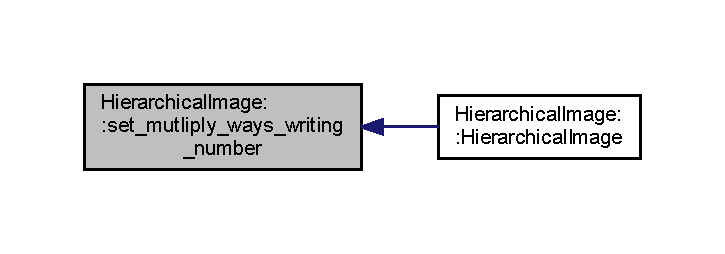
\includegraphics[width=348pt]{class_hierarchical_image_a2f5b6691db32f8af8fff11a4982e88b9_icgraph}
\end{center}
\end{figure}


\index{Hierarchical\-Image@{Hierarchical\-Image}!write\-\_\-image@{write\-\_\-image}}
\index{write\-\_\-image@{write\-\_\-image}!HierarchicalImage@{Hierarchical\-Image}}
\subsubsection[{write\-\_\-image}]{\setlength{\rightskip}{0pt plus 5cm}template$<$typename T , size\-\_\-t memory\-\_\-usage$>$ bool {\bf Hierarchical\-Image}$<$ T, memory\-\_\-usage $>$\-::write\-\_\-image (
\begin{DoxyParamCaption}
\item[{const char $\ast$}]{file\-\_\-name}
\end{DoxyParamCaption}
)\hspace{0.3cm}{\ttfamily [virtual]}}\label{class_hierarchical_image_a6ade13ae295516b5a899498c6800451d}
\begin{DoxyNote}{注解}
file\-\_\-name must has the extension \char`\"{}.\-bigimage\char`\"{} 
\end{DoxyNote}


重载 {\bf Blockwise\-Image$<$ T, memory\-\_\-usage $>$} \doxyref{}{p.}{class_blockwise_image_a64f3e966d516c8b039bd9f4c8685055c} .



在文件 {\bf Hierarchical\-Image.\-hpp} 第  行定义.



\subsection{友元及相关函数文档}
\index{Hierarchical\-Image@{Hierarchical\-Image}!get\-\_\-hierarchical\-\_\-image\-\_\-by\-\_\-meomory\-\_\-usage@{get\-\_\-hierarchical\-\_\-image\-\_\-by\-\_\-meomory\-\_\-usage}}
\index{get\-\_\-hierarchical\-\_\-image\-\_\-by\-\_\-meomory\-\_\-usage@{get\-\_\-hierarchical\-\_\-image\-\_\-by\-\_\-meomory\-\_\-usage}!HierarchicalImage@{Hierarchical\-Image}}
\subsubsection[{get\-\_\-hierarchical\-\_\-image\-\_\-by\-\_\-meomory\-\_\-usage}]{\setlength{\rightskip}{0pt plus 5cm}template$<$typename T $>$ boost\-::shared\-\_\-ptr$<$ {\bf Giant\-Image\-Interface}$<$ T $>$ $>$ get\-\_\-hierarchical\-\_\-image\-\_\-by\-\_\-meomory\-\_\-usage (
\begin{DoxyParamCaption}
\item[{unsigned}]{memory\-\_\-usage, }
\item[{size\-\_\-t}]{rows, }
\item[{size\-\_\-t}]{cols, }
\item[{size\-\_\-t}]{mini\-\_\-rows, }
\item[{size\-\_\-t}]{mini\-\_\-cols, }
\item[{boost\-::shared\-\_\-ptr$<$ {\bf Index\-Method\-Interface} $>$}]{method = {\ttfamily boost\-:\-:shared\-\_\-ptr$<${\bf Index\-Method\-Interface}$>$()}}
\end{DoxyParamCaption}
)\hspace{0.3cm}{\ttfamily [related]}}\label{class_hierarchical_image_a743b80da5ae98d79af3fd143a3a7fb18}


return the hierarchical image by memroy\-\_\-usage, maximum support 4\-G 


\begin{DoxyParams}{参数}
{\em memory\-\_\-usage} & the memory usage of the main memory \\
\hline
{\em method} & the index method shared\-\_\-ptr object \\
\hline
{\em rows} & the image total rows \\
\hline
{\em cols} & the image total cols \\
\hline
{\em mini\-\_\-rows} & the minimum size image rows \\
\hline
{\em mini\-\_\-cols} & the minimum size image cols \\
\hline
\end{DoxyParams}
\begin{DoxyReturn}{返回}
the shared\-\_\-ptr of the \doxyref{Giant\-Image\-Interface}{p.}{class_giant_image_interface} object which indeed is a \doxyref{Hierarchical\-Image}{p.}{class_hierarchical_image} object 
\end{DoxyReturn}


在文件 {\bf Hierarchical\-Image.\-h} 第  行定义.



\subsection{类成员变量说明}
\index{Hierarchical\-Image@{Hierarchical\-Image}!concurrent\-\_\-number@{concurrent\-\_\-number}}
\index{concurrent\-\_\-number@{concurrent\-\_\-number}!HierarchicalImage@{Hierarchical\-Image}}
\subsubsection[{concurrent\-\_\-number}]{\setlength{\rightskip}{0pt plus 5cm}template$<$typename T, size\-\_\-t memory\-\_\-usage = 64$>$ size\-\_\-t {\bf Hierarchical\-Image}$<$ T, memory\-\_\-usage $>$\-::concurrent\-\_\-number\hspace{0.3cm}{\ttfamily [protected]}}\label{class_hierarchical_image_a83791665a03876e2e0927035edb35823}
the number for writing image data files in concurrently 

在文件 {\bf Hierarchical\-Image.\-h} 第  行定义.

\index{Hierarchical\-Image@{Hierarchical\-Image}!img\-\_\-current\-\_\-level\-\_\-size@{img\-\_\-current\-\_\-level\-\_\-size}}
\index{img\-\_\-current\-\_\-level\-\_\-size@{img\-\_\-current\-\_\-level\-\_\-size}!HierarchicalImage@{Hierarchical\-Image}}
\subsubsection[{img\-\_\-current\-\_\-level\-\_\-size}]{\setlength{\rightskip}{0pt plus 5cm}template$<$typename T, size\-\_\-t memory\-\_\-usage = 64$>$ {\bf Size} {\bf Hierarchical\-Image}$<$ T, memory\-\_\-usage $>$\-::img\-\_\-current\-\_\-level\-\_\-size\hspace{0.3cm}{\ttfamily [protected]}}\label{class_hierarchical_image_a9a595586f85d45a1964600eb7ec4559f}
the image current level 

在文件 {\bf Hierarchical\-Image.\-h} 第  行定义.

\index{Hierarchical\-Image@{Hierarchical\-Image}!img\-\_\-data\-\_\-path@{img\-\_\-data\-\_\-path}}
\index{img\-\_\-data\-\_\-path@{img\-\_\-data\-\_\-path}!HierarchicalImage@{Hierarchical\-Image}}
\subsubsection[{img\-\_\-data\-\_\-path}]{\setlength{\rightskip}{0pt plus 5cm}template$<$typename T, size\-\_\-t memory\-\_\-usage = 64$>$ std\-::string {\bf Hierarchical\-Image}$<$ T, memory\-\_\-usage $>$\-::img\-\_\-data\-\_\-path\hspace{0.3cm}{\ttfamily [protected]}}\label{class_hierarchical_image_a79a42b409bae6f95caeddfe9bd20d3bf}
the data of the image file data 

在文件 {\bf Hierarchical\-Image.\-h} 第  行定义.



该类的文档由以下文件生成\-:\begin{DoxyCompactItemize}
\item 
D\-:/\-Out\-\_\-\-Of\-\_\-\-Core\-\_\-\-Git/src/Hierarchical\-Image.\-h\item 
D\-:/\-Out\-\_\-\-Of\-\_\-\-Core\-\_\-\-Git/src/Hierarchical\-Image.\-hpp\end{DoxyCompactItemize}

\section{Image\-File\-L\-R\-U$<$ T $>$ 模板类 参考}
\label{class_image_file_l_r_u}\index{Image\-File\-L\-R\-U$<$ T $>$@{Image\-File\-L\-R\-U$<$ T $>$}}


Implement the saving the big image file cache in lru algorithm.  




{\ttfamily \#include $<$Lru.\-hpp$>$}

\subsection*{类}
\begin{DoxyCompactItemize}
\item 
struct {\bfseries Value\-Type}
\end{DoxyCompactItemize}
\subsection*{Public 成员函数}
\begin{DoxyCompactItemize}
\item 
void {\bfseries init} (int \-\_\-file\-\_\-cell\-\_\-numbers, int \-\_\-file\-\_\-cache\-\_\-numbers)\label{class_image_file_l_r_u_ae4c6a31f48efd1b4c1d5b8af3f498a48}

\item 
{\bf Image\-File\-L\-R\-U} (int \-\_\-file\-\_\-cell\-\_\-numbers=0, int \-\_\-file\-\_\-cache\-\_\-numbers=16)
\begin{DoxyCompactList}\small\item\em initialize the lru manager \end{DoxyCompactList}\item 
bool {\bf exists} (const std\-::string \&file\-\_\-name) const \label{class_image_file_l_r_u_ac445f797cf8143332d66adac5ef952a8}

\begin{DoxyCompactList}\small\item\em checks whether the file\-\_\-name is in the file cache \end{DoxyCompactList}\item 
int {\bf find} (const std\-::string \&file\-\_\-name) const \label{class_image_file_l_r_u_ad7d29e17153c91e1c8a729a14d66d8de}

\begin{DoxyCompactList}\small\item\em find the index of the file\-\_\-name in the lru manager, if not exist, return npos \end{DoxyCompactList}\item 
int {\bf put\-\_\-into\-\_\-lru} (const std\-::string \&file\-\_\-name)
\begin{DoxyCompactList}\small\item\em put the file\-\_\-name into the lru manager, and return the index of the specific file\-\_\-name in the lru manager. \end{DoxyCompactList}\item 
bool {\bf write\-\_\-back\-\_\-data} (int index)
\begin{DoxyCompactList}\small\item\em write the index data into the file system \end{DoxyCompactList}\item 
void {\bf update\-\_\-count} (int index)\label{class_image_file_l_r_u_ae7d7d7d92658229946ab5d2ee31b86a8}

\begin{DoxyCompactList}\small\item\em update the count of all the file cache count, the specific index is set to zero \end{DoxyCompactList}\item 
const std\-::vector$<$ T $>$ \& {\bfseries get\-\_\-const\-\_\-data} (int index) const \label{class_image_file_l_r_u_a6cff9ae749d778bd9b36a4064b55bac5}

\item 
std\-::vector$<$ T $>$ \& {\bfseries get\-\_\-data} (int index)\label{class_image_file_l_r_u_a6dd8ca2125fc0212d4b4d56c7ade97b6}

\end{DoxyCompactItemize}
\subsection*{静态 Public 属性}
\begin{DoxyCompactItemize}
\item 
static const int {\bf npos} = -\/1
\end{DoxyCompactItemize}


\subsection{详细描述}
\subsubsection*{template$<$typename T$>$class Image\-File\-L\-R\-U$<$ T $>$}

Implement the saving the big image file cache in lru algorithm. 

\begin{DoxySeeAlso}{参见}
\doxyref{Disk\-Big\-Image}{p.}{class_disk_big_image}
\end{DoxySeeAlso}

\begin{DoxyTemplParams}{Template Parameters}
{\em T} & The type of the image cells \\
\hline
\end{DoxyTemplParams}


在文件 {\bf Lru.\-hpp} 第  行定义.



\subsection{构造及析构函数说明}
\index{Image\-File\-L\-R\-U@{Image\-File\-L\-R\-U}!Image\-File\-L\-R\-U@{Image\-File\-L\-R\-U}}
\index{Image\-File\-L\-R\-U@{Image\-File\-L\-R\-U}!ImageFileLRU@{Image\-File\-L\-R\-U}}
\subsubsection[{Image\-File\-L\-R\-U}]{\setlength{\rightskip}{0pt plus 5cm}template$<$typename T$>$ {\bf Image\-File\-L\-R\-U}$<$ T $>$\-::{\bf Image\-File\-L\-R\-U} (
\begin{DoxyParamCaption}
\item[{int}]{\-\_\-file\-\_\-cell\-\_\-numbers = {\ttfamily 0}, }
\item[{int}]{\-\_\-file\-\_\-cache\-\_\-numbers = {\ttfamily 16}}
\end{DoxyParamCaption}
)\hspace{0.3cm}{\ttfamily [inline]}}\label{class_image_file_l_r_u_abf84a19c79e7ee0644f1234047707075}


initialize the lru manager 


\begin{DoxyParams}{参数}
{\em \-\_\-file\-\_\-cell\-\_\-numbers} & the cell number in one file \\
\hline
{\em \-\_\-file\-\_\-cache\-\_\-numbers} & the file cache number \\
\hline
\end{DoxyParams}


在文件 {\bf Lru.\-hpp} 第  行定义.



\subsection{成员函数说明}
\index{Image\-File\-L\-R\-U@{Image\-File\-L\-R\-U}!put\-\_\-into\-\_\-lru@{put\-\_\-into\-\_\-lru}}
\index{put\-\_\-into\-\_\-lru@{put\-\_\-into\-\_\-lru}!ImageFileLRU@{Image\-File\-L\-R\-U}}
\subsubsection[{put\-\_\-into\-\_\-lru}]{\setlength{\rightskip}{0pt plus 5cm}template$<$typename T$>$ int {\bf Image\-File\-L\-R\-U}$<$ T $>$\-::put\-\_\-into\-\_\-lru (
\begin{DoxyParamCaption}
\item[{const std\-::string \&}]{file\-\_\-name}
\end{DoxyParamCaption}
)\hspace{0.3cm}{\ttfamily [inline]}}\label{class_image_file_l_r_u_a6f82c20ef87c11c8711b8d10f7c08704}


put the file\-\_\-name into the lru manager, and return the index of the specific file\-\_\-name in the lru manager. 

\begin{DoxyReturn}{返回}
the index of the image file. 
\end{DoxyReturn}
\begin{DoxyNote}{注解}
if fails to put the file into lru manager, the return value is \doxyref{Image\-File\-L\-R\-U\-::npos}{p.}{class_image_file_l_r_u_a883a4e3cf0cd1c9922c5185c6df850a6} 
\end{DoxyNote}


在文件 {\bf Lru.\-hpp} 第  行定义.

\index{Image\-File\-L\-R\-U@{Image\-File\-L\-R\-U}!write\-\_\-back\-\_\-data@{write\-\_\-back\-\_\-data}}
\index{write\-\_\-back\-\_\-data@{write\-\_\-back\-\_\-data}!ImageFileLRU@{Image\-File\-L\-R\-U}}
\subsubsection[{write\-\_\-back\-\_\-data}]{\setlength{\rightskip}{0pt plus 5cm}template$<$typename T$>$ bool {\bf Image\-File\-L\-R\-U}$<$ T $>$\-::write\-\_\-back\-\_\-data (
\begin{DoxyParamCaption}
\item[{int}]{index}
\end{DoxyParamCaption}
)\hspace{0.3cm}{\ttfamily [inline]}}\label{class_image_file_l_r_u_af0558f8a6e29adda0b155e1323626311}


write the index data into the file system 

\begin{DoxyReturn}{返回}
whether write successfully 
\end{DoxyReturn}


在文件 {\bf Lru.\-hpp} 第  行定义.



这是这个函数的调用关系图\-:\nopagebreak
\begin{figure}[H]
\begin{center}
\leavevmode
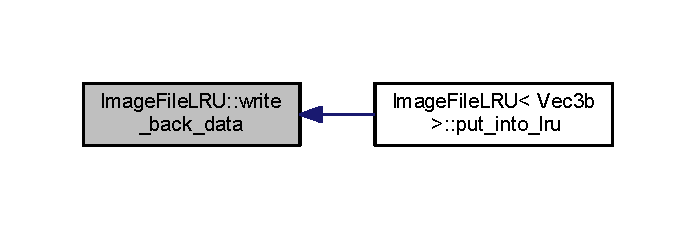
\includegraphics[width=334pt]{class_image_file_l_r_u_af0558f8a6e29adda0b155e1323626311_icgraph}
\end{center}
\end{figure}




\subsection{类成员变量说明}
\index{Image\-File\-L\-R\-U@{Image\-File\-L\-R\-U}!npos@{npos}}
\index{npos@{npos}!ImageFileLRU@{Image\-File\-L\-R\-U}}
\subsubsection[{npos}]{\setlength{\rightskip}{0pt plus 5cm}template$<$typename T$>$ const int {\bf Image\-File\-L\-R\-U}$<$ T $>$\-::npos = -\/1\hspace{0.3cm}{\ttfamily [static]}}\label{class_image_file_l_r_u_a883a4e3cf0cd1c9922c5185c6df850a6}
the npos means invalid index 

在文件 {\bf Lru.\-hpp} 第  行定义.



该类的文档由以下文件生成\-:\begin{DoxyCompactItemize}
\item 
D\-:/\-Out\-\_\-\-Of\-\_\-\-Core\-\_\-\-Git/src/Lru.\-hpp\end{DoxyCompactItemize}

\section{Image\-Interface$<$ T $>$ 模板类 参考}
\label{class_image_interface}\index{Image\-Interface$<$ T $>$@{Image\-Interface$<$ T $>$}}


The Basic Image Interface contains of several basic image processing functions.  




{\ttfamily \#include $<$Image\-Interface.\-h$>$}



类 Image\-Interface$<$ T $>$ 继承关系图\-:\nopagebreak
\begin{figure}[H]
\begin{center}
\leavevmode
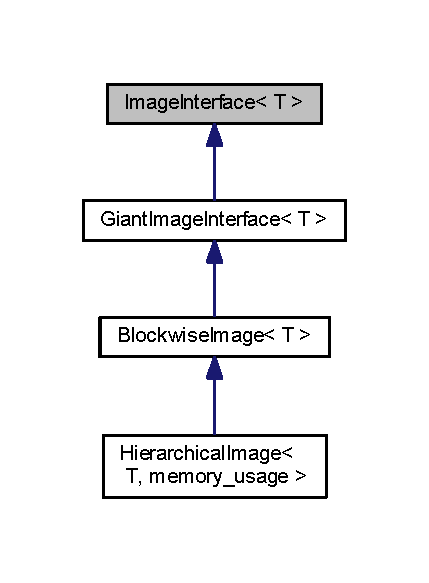
\includegraphics[width=206pt]{class_image_interface__inherit__graph}
\end{center}
\end{figure}


Image\-Interface$<$ T $>$ 的协作图\-:\nopagebreak
\begin{figure}[H]
\begin{center}
\leavevmode
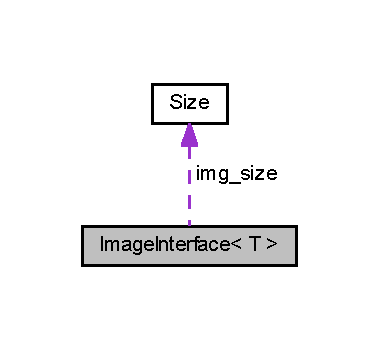
\includegraphics[width=182pt]{class_image_interface__coll__graph}
\end{center}
\end{figure}
\subsection*{Public 成员函数}
\begin{DoxyCompactItemize}
\item 
virtual bool {\bf init} (int rows, int cols)=0
\begin{DoxyCompactList}\small\item\em Initialize the image size, and allocate the memory for saving the image. \end{DoxyCompactList}\item 
virtual bool {\bf reset} ()=0\label{class_image_interface_a7c46834fca2a54671129e51035e4da82}

\begin{DoxyCompactList}\small\item\em Clear the image data. \end{DoxyCompactList}\item 
virtual bool {\bf write\-\_\-image} (const char $\ast$file\-\_\-name)=0
\begin{DoxyCompactList}\small\item\em Write the image to the disk. \end{DoxyCompactList}\item 
virtual bool {\bfseries write\-\_\-image} (const std\-::string \&file\-\_\-name)=0\label{class_image_interface_ad15d73a867929d830d66db206f418779}

\item 
virtual T \& {\bf get\-\_\-pixel} (int row, int col)=0
\begin{DoxyCompactList}\small\item\em Get the pixel of the point (row, col), or just write code like image(row, col) to get the image pixel. \end{DoxyCompactList}\item 
virtual const T \& {\bfseries get\-\_\-pixel} (int row, int col) const =0\label{class_image_interface_afde188c9465ecf66e7b736e03fb625c6}

\item 
virtual T \& {\bfseries operator()} (int row, int col)=0\label{class_image_interface_a15e127520b9b598db90f68453b18c678}

\item 
virtual const T \& {\bfseries operator()} (int row, int col) const =0\label{class_image_interface_abd4e6863efd75d01793072296cb59476}

\item 
virtual bool {\bf get\-\_\-pixels} (int start\-\_\-row, int start\-\_\-col, int rows, int cols, std\-::vector$<$ T $>$ \&data) const =0
\begin{DoxyCompactList}\small\item\em Get the range image data. \end{DoxyCompactList}\item 
virtual bool {\bfseries set\-\_\-pixels} (int start\-\_\-row, int start\-\_\-col, int rows, int cols, const std\-::vector$<$ T $>$ \&data)=0\label{class_image_interface_ae7af79229968b890b8e02431ccc7e9bb}

\item 
virtual bool {\bf set\-\_\-pixels} (int start\-\_\-row, int start\-\_\-col, int rows, int cols, const T clear\-\_\-value)=0
\begin{DoxyCompactList}\small\item\em set the range image data with a const value \end{DoxyCompactList}\item 
size\-\_\-t {\bfseries get\-\_\-image\-\_\-cols} () const \label{class_image_interface_a32131143cea03bf8717221d111107744}

\item 
size\-\_\-t {\bfseries get\-\_\-image\-\_\-rows} () const \label{class_image_interface_ac23652bfec86e2b16e645243e2f2de76}

\end{DoxyCompactItemize}
\subsection*{Protected 属性}
\begin{DoxyCompactItemize}
\item 
{\bf Size} {\bfseries img\-\_\-size}\label{class_image_interface_a2a9ef3aa0859982b8eb2b8e8f73ab8ed}

\end{DoxyCompactItemize}


\subsection{详细描述}
\subsubsection*{template$<$typename T$>$class Image\-Interface$<$ T $>$}

The Basic Image Interface contains of several basic image processing functions. 


\begin{DoxyTemplParams}{Template Parameters}
{\em T} & The type of the image cells \\
\hline
\end{DoxyTemplParams}


在文件 {\bf Image\-Interface.\-h} 第  行定义.



\subsection{成员函数说明}
\index{Image\-Interface@{Image\-Interface}!get\-\_\-pixel@{get\-\_\-pixel}}
\index{get\-\_\-pixel@{get\-\_\-pixel}!ImageInterface@{Image\-Interface}}
\subsubsection[{get\-\_\-pixel}]{\setlength{\rightskip}{0pt plus 5cm}template$<$typename T $>$ virtual T\& {\bf Image\-Interface}$<$ T $>$\-::get\-\_\-pixel (
\begin{DoxyParamCaption}
\item[{int}]{row, }
\item[{int}]{col}
\end{DoxyParamCaption}
)\hspace{0.3cm}{\ttfamily [pure virtual]}}\label{class_image_interface_af5fc491e3c7bb401a3591de26049bc7d}


Get the pixel of the point (row, col), or just write code like image(row, col) to get the image pixel. 

\begin{DoxyReturn}{返回}
The reference of the image pixel 
\end{DoxyReturn}
\begin{DoxyWarning}{警告}
In release mode, the row and col param must be valid, otherwise there will be an exception 
\end{DoxyWarning}


在 {\bf Blockwise\-Image$<$ T, memory\-\_\-usage $>$} \doxyref{}{p.}{class_blockwise_image_a110d2b1c0d6ac08cb8e66f74b32bd72d} 内被实现.

\index{Image\-Interface@{Image\-Interface}!get\-\_\-pixels@{get\-\_\-pixels}}
\index{get\-\_\-pixels@{get\-\_\-pixels}!ImageInterface@{Image\-Interface}}
\subsubsection[{get\-\_\-pixels}]{\setlength{\rightskip}{0pt plus 5cm}template$<$typename T $>$ virtual bool {\bf Image\-Interface}$<$ T $>$\-::get\-\_\-pixels (
\begin{DoxyParamCaption}
\item[{int}]{start\-\_\-row, }
\item[{int}]{start\-\_\-col, }
\item[{int}]{rows, }
\item[{int}]{cols, }
\item[{std\-::vector$<$ T $>$ \&}]{data}
\end{DoxyParamCaption}
) const\hspace{0.3cm}{\ttfamily [pure virtual]}}\label{class_image_interface_a2a2254be220b4a4bb6effed70d61c6df}


Get the range image data. 


\begin{DoxyParams}{参数}
{\em start\-\_\-row} & The left-\/corner point row \\
\hline
{\em start\-\_\-col} & The left-\/corner point col \\
\hline
{\em rows} & The row scope of the range, thus the rows get is [start\-\_\-row, start\-\_\-row + rows) \\
\hline
{\em cols} & The col scope of the range \\
\hline
{\em data} & [Out] Returns the image data vector \\
\hline
\end{DoxyParams}
\begin{DoxyNote}{注解}
the data doesn't need to allocate any memory 
\end{DoxyNote}
\begin{DoxyReturn}{返回}
Whether get the data successfully 
\end{DoxyReturn}


在 {\bf Blockwise\-Image$<$ T, memory\-\_\-usage $>$} \doxyref{}{p.}{class_blockwise_image_a91c1d0be2ef9ab54f1a5f9e706e13174} 内被实现.

\index{Image\-Interface@{Image\-Interface}!init@{init}}
\index{init@{init}!ImageInterface@{Image\-Interface}}
\subsubsection[{init}]{\setlength{\rightskip}{0pt plus 5cm}template$<$typename T $>$ virtual bool {\bf Image\-Interface}$<$ T $>$\-::init (
\begin{DoxyParamCaption}
\item[{int}]{rows, }
\item[{int}]{cols}
\end{DoxyParamCaption}
)\hspace{0.3cm}{\ttfamily [pure virtual]}}\label{class_image_interface_a6f59d1e81ab88e0ca2c5d4b6a2e98ae5}


Initialize the image size, and allocate the memory for saving the image. 

\begin{DoxyReturn}{返回}
Whether initialize successfully 
\end{DoxyReturn}


在 {\bf Blockwise\-Image$<$ T, memory\-\_\-usage $>$} \doxyref{}{p.}{class_blockwise_image_a9bbeb6df0a51caf818d100c3e869f45b} 内被实现.

\index{Image\-Interface@{Image\-Interface}!set\-\_\-pixels@{set\-\_\-pixels}}
\index{set\-\_\-pixels@{set\-\_\-pixels}!ImageInterface@{Image\-Interface}}
\subsubsection[{set\-\_\-pixels}]{\setlength{\rightskip}{0pt plus 5cm}template$<$typename T $>$ virtual bool {\bf Image\-Interface}$<$ T $>$\-::set\-\_\-pixels (
\begin{DoxyParamCaption}
\item[{int}]{start\-\_\-row, }
\item[{int}]{start\-\_\-col, }
\item[{int}]{rows, }
\item[{int}]{cols, }
\item[{const T}]{clear\-\_\-value}
\end{DoxyParamCaption}
)\hspace{0.3cm}{\ttfamily [pure virtual]}}\label{class_image_interface_aa35f6a2c062df7a9796fc672b16cafc8}


set the range image data with a const value 


\begin{DoxyParams}{参数}
{\em start\-\_\-row} & The left-\/corner point row \\
\hline
{\em start\-\_\-col} & The left-\/corner point col \\
\hline
{\em rows} & The row scope of the range, thus the rows get is [start\-\_\-row, start\-\_\-row + rows) \\
\hline
{\em cols} & The col scope of the range \\
\hline
{\em clear\-\_\-value} & the value that with to fill the image range \\
\hline
\end{DoxyParams}
\begin{DoxyReturn}{返回}
Whether set successfully 
\end{DoxyReturn}


在 {\bf Blockwise\-Image$<$ T, memory\-\_\-usage $>$} \doxyref{}{p.}{class_blockwise_image_ac4da5390aa20631c1f0e88b6a93cfead} 内被实现.

\index{Image\-Interface@{Image\-Interface}!write\-\_\-image@{write\-\_\-image}}
\index{write\-\_\-image@{write\-\_\-image}!ImageInterface@{Image\-Interface}}
\subsubsection[{write\-\_\-image}]{\setlength{\rightskip}{0pt plus 5cm}template$<$typename T $>$ virtual bool {\bf Image\-Interface}$<$ T $>$\-::write\-\_\-image (
\begin{DoxyParamCaption}
\item[{const char $\ast$}]{file\-\_\-name}
\end{DoxyParamCaption}
)\hspace{0.3cm}{\ttfamily [pure virtual]}}\label{class_image_interface_ad5c2431a4b31bcb600ba996858efa620}


Write the image to the disk. 


\begin{DoxyParams}{参数}
{\em file\-\_\-name} & The name of the image file \\
\hline
\end{DoxyParams}
\begin{DoxyReturn}{返回}
Whether write successfully 
\end{DoxyReturn}


在 {\bf Blockwise\-Image$<$ T, memory\-\_\-usage $>$} \doxyref{}{p.}{class_blockwise_image_a64f3e966d516c8b039bd9f4c8685055c} , 以及 {\bf Hierarchical\-Image$<$ T, memory\-\_\-usage $>$} \doxyref{}{p.}{class_hierarchical_image_a6ade13ae295516b5a899498c6800451d} 内被实现.



该类的文档由以下文件生成\-:\begin{DoxyCompactItemize}
\item 
D\-:/\-Out\-\_\-\-Of\-\_\-\-Core\-\_\-\-Git/src/Image\-Interface.\-h\end{DoxyCompactItemize}

\section{Index\-Method\-Interface类 参考}
\label{class_index_method_interface}\index{Index\-Method\-Interface@{Index\-Method\-Interface}}


The basic functions of the indexing method.  




{\ttfamily \#include $<$Index\-Method\-Interface.\-h$>$}



类 Index\-Method\-Interface 继承关系图\-:\nopagebreak
\begin{figure}[H]
\begin{center}
\leavevmode
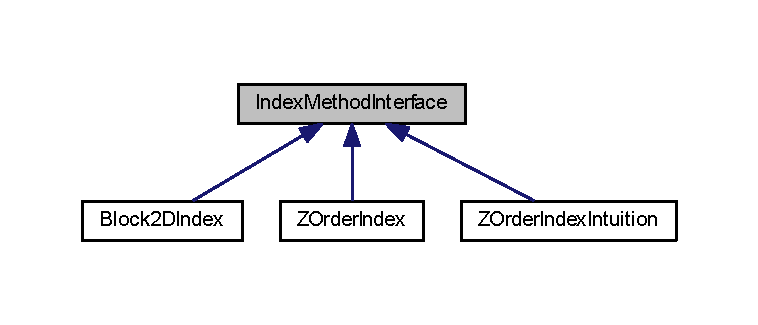
\includegraphics[width=350pt]{class_index_method_interface__inherit__graph}
\end{center}
\end{figure}
\subsection*{Public 类型}
\begin{DoxyCompactItemize}
\item 
typedef int64 {\bf Index\-Type}
\item 
typedef size\-\_\-t {\bf Row\-Major\-Index\-Type}
\end{DoxyCompactItemize}
\subsection*{Public 成员函数}
\begin{DoxyCompactItemize}
\item 
virtual {\bf Index\-Type} {\bf get\-\_\-index} ({\bf Row\-Major\-Index\-Type} row, {\bf Row\-Major\-Index\-Type} col) const =0\label{class_index_method_interface_ac711b80e04bd6fdf4cd5365ed8c9525b}

\begin{DoxyCompactList}\small\item\em get the index of row-\/major index (row, col) \end{DoxyCompactList}\item 
virtual {\bf Row\-Major\-Point} {\bf get\-\_\-origin\-\_\-index} ({\bf Index\-Type} index) const =0
\begin{DoxyCompactList}\small\item\em get the original row-\/major index \end{DoxyCompactList}\item 
virtual {\bf Index\-Type} {\bf get\-\_\-row\-\_\-result} ({\bf Row\-Major\-Index\-Type} row\-\_\-index) const =0
\begin{DoxyCompactList}\small\item\em get the row result from just the row index (for using row-\/major like loop). \end{DoxyCompactList}\item 
virtual {\bf Index\-Type} {\bf get\-\_\-index\-\_\-by\-\_\-row\-\_\-result} ({\bf Index\-Type} row\-\_\-result, {\bf Row\-Major\-Index\-Type} col\-\_\-index) const =0
\begin{DoxyCompactList}\small\item\em get the index from row result and col index \end{DoxyCompactList}\item 
virtual {\bf Index\-Type} {\bf get\-\_\-max\-\_\-index} () const =0
\begin{DoxyCompactList}\small\item\em get the maximum index, often used to ensure the size of the container \end{DoxyCompactList}\item 
virtual std\-::string {\bf get\-\_\-index\-\_\-method\-\_\-name} () const =0\label{class_index_method_interface_a020f398f97b2bdc041101c44e71cbcbf}

\begin{DoxyCompactList}\small\item\em get the index method name for identify different method \end{DoxyCompactList}\end{DoxyCompactItemize}


\subsection{详细描述}
The basic functions of the indexing method. 

在文件 {\bf Index\-Method\-Interface.\-h} 第  行定义.



\subsection{成员类型定义说明}
\index{Index\-Method\-Interface@{Index\-Method\-Interface}!Index\-Type@{Index\-Type}}
\index{Index\-Type@{Index\-Type}!IndexMethodInterface@{Index\-Method\-Interface}}
\subsubsection[{Index\-Type}]{\setlength{\rightskip}{0pt plus 5cm}typedef int64 {\bf Index\-Method\-Interface\-::\-Index\-Type}}\label{class_index_method_interface_ab7022c5b65707f1d10a71f45134b21ba}
the type of all the index 

在文件 {\bf Index\-Method\-Interface.\-h} 第  行定义.

\index{Index\-Method\-Interface@{Index\-Method\-Interface}!Row\-Major\-Index\-Type@{Row\-Major\-Index\-Type}}
\index{Row\-Major\-Index\-Type@{Row\-Major\-Index\-Type}!IndexMethodInterface@{Index\-Method\-Interface}}
\subsubsection[{Row\-Major\-Index\-Type}]{\setlength{\rightskip}{0pt plus 5cm}typedef size\-\_\-t {\bf Index\-Method\-Interface\-::\-Row\-Major\-Index\-Type}}\label{class_index_method_interface_ab8dd67018f74893f816260b05a5246b3}
the type of row-\/major like index 

在文件 {\bf Index\-Method\-Interface.\-h} 第  行定义.



\subsection{成员函数说明}
\index{Index\-Method\-Interface@{Index\-Method\-Interface}!get\-\_\-index\-\_\-by\-\_\-row\-\_\-result@{get\-\_\-index\-\_\-by\-\_\-row\-\_\-result}}
\index{get\-\_\-index\-\_\-by\-\_\-row\-\_\-result@{get\-\_\-index\-\_\-by\-\_\-row\-\_\-result}!IndexMethodInterface@{Index\-Method\-Interface}}
\subsubsection[{get\-\_\-index\-\_\-by\-\_\-row\-\_\-result}]{\setlength{\rightskip}{0pt plus 5cm}virtual {\bf Index\-Type} Index\-Method\-Interface\-::get\-\_\-index\-\_\-by\-\_\-row\-\_\-result (
\begin{DoxyParamCaption}
\item[{{\bf Index\-Type}}]{row\-\_\-result, }
\item[{{\bf Row\-Major\-Index\-Type}}]{col\-\_\-index}
\end{DoxyParamCaption}
) const\hspace{0.3cm}{\ttfamily [pure virtual]}}\label{class_index_method_interface_af6fda6db139d00aa3e722fcd20945322}


get the index from row result and col index 


\begin{DoxyParams}{参数}
{\em row\-\_\-result} & the result get from the \doxyref{get\-\_\-row\-\_\-result()}{p.}{class_index_method_interface_aab87157a6dcd40f8d249616829f7ec97} method \\
\hline
{\em col\-\_\-index} & the index of col in the row-\/major format \\
\hline
\end{DoxyParams}
\begin{DoxyReturn}{返回}
the index result combined both the row and col 
\end{DoxyReturn}


在 {\bf Z\-Order\-Index} \doxyref{}{p.}{class_z_order_index_a62ee0e4943a2c13f47eb9065ec056c00},{\bf Z\-Order\-Index\-Intuition} \doxyref{}{p.}{class_z_order_index_intuition_a260c382c65f156a14993c3035adff46c} , 以及 {\bf Block2\-D\-Index} \doxyref{}{p.}{class_block2_d_index_a3ead3723b1619b13e20a4ed14469a32d} 内被实现.

\index{Index\-Method\-Interface@{Index\-Method\-Interface}!get\-\_\-max\-\_\-index@{get\-\_\-max\-\_\-index}}
\index{get\-\_\-max\-\_\-index@{get\-\_\-max\-\_\-index}!IndexMethodInterface@{Index\-Method\-Interface}}
\subsubsection[{get\-\_\-max\-\_\-index}]{\setlength{\rightskip}{0pt plus 5cm}virtual {\bf Index\-Type} Index\-Method\-Interface\-::get\-\_\-max\-\_\-index (
\begin{DoxyParamCaption}
{}
\end{DoxyParamCaption}
) const\hspace{0.3cm}{\ttfamily [pure virtual]}}\label{class_index_method_interface_ad2e684fc1ef5ea505ccbc23278977478}


get the maximum index, often used to ensure the size of the container 

\begin{DoxyReturn}{返回}
the maximum index get from the this indexing method 
\end{DoxyReturn}


在 {\bf Z\-Order\-Index} \doxyref{}{p.}{class_z_order_index_ac9eacf3a0481b0b26e2b98216c04689e},{\bf Z\-Order\-Index\-Intuition} \doxyref{}{p.}{class_z_order_index_intuition_aaf09fc4e8668b254e8d8fb0abcc26719} , 以及 {\bf Block2\-D\-Index} \doxyref{}{p.}{class_block2_d_index_a1cdb7f2f1ca93be4e14cee70f4038160} 内被实现.

\index{Index\-Method\-Interface@{Index\-Method\-Interface}!get\-\_\-origin\-\_\-index@{get\-\_\-origin\-\_\-index}}
\index{get\-\_\-origin\-\_\-index@{get\-\_\-origin\-\_\-index}!IndexMethodInterface@{Index\-Method\-Interface}}
\subsubsection[{get\-\_\-origin\-\_\-index}]{\setlength{\rightskip}{0pt plus 5cm}virtual {\bf Row\-Major\-Point} Index\-Method\-Interface\-::get\-\_\-origin\-\_\-index (
\begin{DoxyParamCaption}
\item[{{\bf Index\-Type}}]{index}
\end{DoxyParamCaption}
) const\hspace{0.3cm}{\ttfamily [pure virtual]}}\label{class_index_method_interface_a44f4553bd06c787d4523c37a9a15fdd3}


get the original row-\/major index 


\begin{DoxyParams}{参数}
{\em index} & the index calculated from \doxyref{get\-\_\-index()}{p.}{class_index_method_interface_ac711b80e04bd6fdf4cd5365ed8c9525b} method \\
\hline
\end{DoxyParams}
\begin{DoxyReturn}{返回}
the row-\/major index (row, col) format 
\end{DoxyReturn}


在 {\bf Z\-Order\-Index} \doxyref{}{p.}{class_z_order_index_a90fb65a322a8b1f28f3a7e3b0ba5fe27},{\bf Z\-Order\-Index\-Intuition} \doxyref{}{p.}{class_z_order_index_intuition_a2cec2d33763c814a1aa638fc755eea68} , 以及 {\bf Block2\-D\-Index} \doxyref{}{p.}{class_block2_d_index_a95e1c7406cabbcf2decde099128a6fa5} 内被实现.

\index{Index\-Method\-Interface@{Index\-Method\-Interface}!get\-\_\-row\-\_\-result@{get\-\_\-row\-\_\-result}}
\index{get\-\_\-row\-\_\-result@{get\-\_\-row\-\_\-result}!IndexMethodInterface@{Index\-Method\-Interface}}
\subsubsection[{get\-\_\-row\-\_\-result}]{\setlength{\rightskip}{0pt plus 5cm}virtual {\bf Index\-Type} Index\-Method\-Interface\-::get\-\_\-row\-\_\-result (
\begin{DoxyParamCaption}
\item[{{\bf Row\-Major\-Index\-Type}}]{row\-\_\-index}
\end{DoxyParamCaption}
) const\hspace{0.3cm}{\ttfamily [pure virtual]}}\label{class_index_method_interface_aab87157a6dcd40f8d249616829f7ec97}


get the row result from just the row index (for using row-\/major like loop). 


\begin{DoxyPre}
Using this method for some kind of optimization when using row-major like loop 
for example:    
for(size\_t row = 0; row < rows; ++row) \{ 
        IndexType row\_result = get\_row\_result(row);
        for(size\_t col = 0; col < cols; ++col) \{ 
                IndexType index = get\_index\_by\_row\_result(row\_result, col); 
        \} 
\} 
\end{DoxyPre}



\begin{DoxyParams}{参数}
{\em row\-\_\-index} & the index of row in the row-\/major format \\
\hline
\end{DoxyParams}
\begin{DoxyReturn}{返回}
the row result 
\end{DoxyReturn}


在 {\bf Z\-Order\-Index} \doxyref{}{p.}{class_z_order_index_ae6448044c3c190826a85c29eac950b86},{\bf Z\-Order\-Index\-Intuition} \doxyref{}{p.}{class_z_order_index_intuition_a681922974bbe3800d01345c9a357238e} , 以及 {\bf Block2\-D\-Index} \doxyref{}{p.}{class_block2_d_index_a96c5893d835bf952463cef1398654361} 内被实现.



该类的文档由以下文件生成\-:\begin{DoxyCompactItemize}
\item 
D\-:/\-Out\-\_\-\-Of\-\_\-\-Core\-\_\-\-Git/src/Index\-Method\-Interface.\-h\end{DoxyCompactItemize}

\section{Pixel\-Element$<$ T $>$ 模板结构体 参考}
\label{struct_pixel_element}\index{Pixel\-Element$<$ T $>$@{Pixel\-Element$<$ T $>$}}


Pixel\-Element$<$ T $>$ 的协作图\-:\nopagebreak
\begin{figure}[H]
\begin{center}
\leavevmode
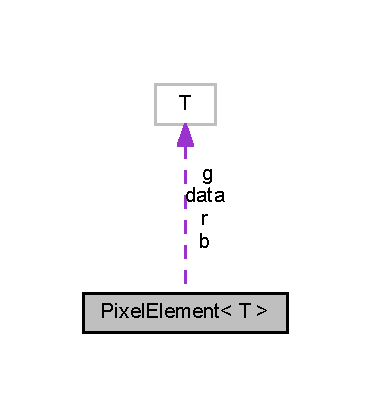
\includegraphics[width=178pt]{struct_pixel_element__coll__graph}
\end{center}
\end{figure}
\subsection*{Public 属性}
\begin{DoxyCompactItemize}
\item 
\begin{tabbing}
xx\=xx\=xx\=xx\=xx\=xx\=xx\=xx\=xx\=\kill
union \{\\
\>struct \{\\
\>\>T {\bfseries r}\\
\>\>T {\bfseries g}\\
\>\>T {\bfseries b}\\
\>\} \label{union_pixel_element_1_1@0_acb0a52d4faf6fe843e22eaec64e2d488}
\\
\>T {\bfseries data} [3]\\
\}; \label{struct_pixel_element_a1472a92dc3ce2319853f75bec0ac742f}
\\

\end{tabbing}\end{DoxyCompactItemize}


\subsection{详细描述}
\subsubsection*{template$<$typename T$>$struct Pixel\-Element$<$ T $>$}

\begin{Desc}
\item[示例\-: ]\par
{\bf test\-Image\-Containter.\-cpp},{\bf Write\-Block\-Wise\-Image.\-cpp} , 以及 {\bf Write\-Hierarchical\-Image.\-cpp}.\end{Desc}


在文件 {\bf Basic\-Type.\-h} 第  行定义.



该结构体的文档由以下文件生成\-:\begin{DoxyCompactItemize}
\item 
D\-:/\-Out\-\_\-\-Of\-\_\-\-Core\-\_\-\-Git/src/Basic\-Type.\-h\end{DoxyCompactItemize}

\section{Row\-Major\-Point结构体 参考}
\label{struct_row_major_point}\index{Row\-Major\-Point@{Row\-Major\-Point}}
\subsection*{Public 成员函数}
\begin{DoxyCompactItemize}
\item 
{\bfseries Row\-Major\-Point} (size\-\_\-t \-\_\-row, size\-\_\-t \-\_\-col)\label{struct_row_major_point_a842420c69222b1e6dc1bbdabe9a04d53}

\end{DoxyCompactItemize}
\subsection*{Public 属性}
\begin{DoxyCompactItemize}
\item 
size\-\_\-t {\bfseries row}\label{struct_row_major_point_ab37a563a22e1827a13b4dbaea2d2ce46}

\item 
size\-\_\-t {\bfseries col}\label{struct_row_major_point_a7c04e4879b6f83c7be6061302c1c7f15}

\end{DoxyCompactItemize}


\subsection{详细描述}
\begin{Desc}
\item[示例\-: ]\par
{\bf test\-Index\-Method.\-cpp}.\end{Desc}


在文件 {\bf Basic\-Type.\-h} 第  行定义.



该结构体的文档由以下文件生成\-:\begin{DoxyCompactItemize}
\item 
D\-:/\-Out\-\_\-\-Of\-\_\-\-Core\-\_\-\-Git/src/Basic\-Type.\-h\end{DoxyCompactItemize}

\section{Size结构体 参考}
\label{struct_size}\index{Size@{Size}}
\subsection*{Public 成员函数}
\begin{DoxyCompactItemize}
\item 
{\bfseries Size} (size\-\_\-t \-\_\-rows=0, size\-\_\-t \-\_\-cols=0)\label{struct_size_a9ca4538e296801bc1e621bfa3d79bf10}

\end{DoxyCompactItemize}
\subsection*{Public 属性}
\begin{DoxyCompactItemize}
\item 
size\-\_\-t {\bfseries cols}\label{struct_size_ad15cd5d15d1cc0cf43dcbae748484237}

\item 
size\-\_\-t {\bfseries rows}\label{struct_size_add52bc013a38bb9089daf65a16341b7f}

\end{DoxyCompactItemize}


\subsection{详细描述}


在文件 {\bf Basic\-Type.\-h} 第  行定义.



该结构体的文档由以下文件生成\-:\begin{DoxyCompactItemize}
\item 
D\-:/\-Out\-\_\-\-Of\-\_\-\-Core\-\_\-\-Git/src/Basic\-Type.\-h\end{DoxyCompactItemize}

\section{Z\-Order\-Index类 参考}
\label{class_z_order_index}\index{Z\-Order\-Index@{Z\-Order\-Index}}


类 Z\-Order\-Index 继承关系图\-:\nopagebreak
\begin{figure}[H]
\begin{center}
\leavevmode
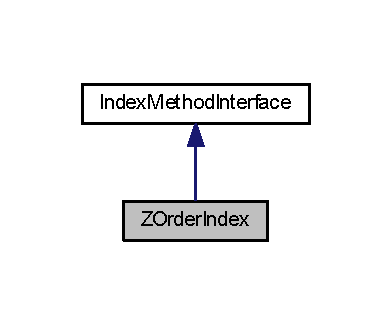
\includegraphics[width=188pt]{class_z_order_index__inherit__graph}
\end{center}
\end{figure}


Z\-Order\-Index 的协作图\-:\nopagebreak
\begin{figure}[H]
\begin{center}
\leavevmode
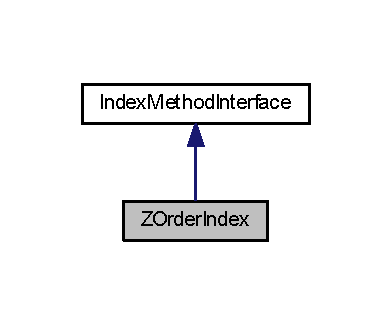
\includegraphics[width=188pt]{class_z_order_index__coll__graph}
\end{center}
\end{figure}
\subsection*{Public 成员函数}
\begin{DoxyCompactItemize}
\item 
{\bf Z\-Order\-Index} ({\bf Row\-Major\-Index\-Type} row\-\_\-size, {\bf Row\-Major\-Index\-Type} col\-\_\-size)
\item 
virtual {\bf Index\-Type} {\bf get\-\_\-row\-\_\-result} ({\bf Row\-Major\-Index\-Type} row\-\_\-index) const 
\begin{DoxyCompactList}\small\item\em get the row result from just the row index (for using row-\/major like loop). \end{DoxyCompactList}\item 
virtual {\bf Index\-Type} {\bf get\-\_\-index\-\_\-by\-\_\-row\-\_\-result} ({\bf Index\-Type} row\-\_\-result, {\bf Row\-Major\-Index\-Type} col\-\_\-index) const 
\begin{DoxyCompactList}\small\item\em get the index from row result and col index \end{DoxyCompactList}\item 
virtual {\bf Index\-Type} {\bf get\-\_\-index} ({\bf Row\-Major\-Index\-Type} row\-\_\-index, {\bf Row\-Major\-Index\-Type} col\-\_\-index) const \label{class_z_order_index_a12b02aba625065238dc1b5789440d9fa}

\begin{DoxyCompactList}\small\item\em get the index of row-\/major index (row, col) \end{DoxyCompactList}\item 
virtual {\bf Row\-Major\-Point} {\bf get\-\_\-origin\-\_\-index} ({\bf Index\-Type} index) const 
\begin{DoxyCompactList}\small\item\em get the original row-\/major index \end{DoxyCompactList}\item 
virtual {\bf Index\-Type} {\bf get\-\_\-max\-\_\-index} () const 
\begin{DoxyCompactList}\small\item\em get the maximum index, often used to ensure the size of the container \end{DoxyCompactList}\item 
virtual std\-::string {\bf get\-\_\-index\-\_\-method\-\_\-name} () const \label{class_z_order_index_aaf9253de07de2076a3de4c2d31210fbd}

\begin{DoxyCompactList}\small\item\em get the index method name for identify different method \end{DoxyCompactList}\end{DoxyCompactItemize}
\subsection*{额外继承的成员函数}


\subsection{详细描述}
\begin{Desc}
\item[示例\-: ]\par
{\bf test\-Image\-Containter.\-cpp} , 以及 {\bf test\-Index\-Method.\-cpp}.\end{Desc}


在文件 {\bf Index\-Method.\-hpp} 第  行定义.



\subsection{构造及析构函数说明}
\index{Z\-Order\-Index@{Z\-Order\-Index}!Z\-Order\-Index@{Z\-Order\-Index}}
\index{Z\-Order\-Index@{Z\-Order\-Index}!ZOrderIndex@{Z\-Order\-Index}}
\subsubsection[{Z\-Order\-Index}]{\setlength{\rightskip}{0pt plus 5cm}Z\-Order\-Index\-::\-Z\-Order\-Index (
\begin{DoxyParamCaption}
\item[{{\bf Row\-Major\-Index\-Type}}]{row\-\_\-size, }
\item[{{\bf Row\-Major\-Index\-Type}}]{col\-\_\-size}
\end{DoxyParamCaption}
)\hspace{0.3cm}{\ttfamily [inline]}}\label{class_z_order_index_a62f71dd133969aea5d5ee8128b405552}

\begin{DoxyParams}{参数}
{\em row\-\_\-size} & the row size of the image \\
\hline
{\em col\-\_\-size} & the col size of the image \\
\hline
\end{DoxyParams}


在文件 {\bf Index\-Method.\-hpp} 第  行定义.



\subsection{成员函数说明}
\index{Z\-Order\-Index@{Z\-Order\-Index}!get\-\_\-index\-\_\-by\-\_\-row\-\_\-result@{get\-\_\-index\-\_\-by\-\_\-row\-\_\-result}}
\index{get\-\_\-index\-\_\-by\-\_\-row\-\_\-result@{get\-\_\-index\-\_\-by\-\_\-row\-\_\-result}!ZOrderIndex@{Z\-Order\-Index}}
\subsubsection[{get\-\_\-index\-\_\-by\-\_\-row\-\_\-result}]{\setlength{\rightskip}{0pt plus 5cm}virtual {\bf Index\-Type} Z\-Order\-Index\-::get\-\_\-index\-\_\-by\-\_\-row\-\_\-result (
\begin{DoxyParamCaption}
\item[{{\bf Index\-Type}}]{row\-\_\-result, }
\item[{{\bf Row\-Major\-Index\-Type}}]{col\-\_\-index}
\end{DoxyParamCaption}
) const\hspace{0.3cm}{\ttfamily [inline]}, {\ttfamily [virtual]}}\label{class_z_order_index_a62ee0e4943a2c13f47eb9065ec056c00}


get the index from row result and col index 


\begin{DoxyParams}{参数}
{\em row\-\_\-result} & the result get from the \doxyref{get\-\_\-row\-\_\-result()}{p.}{class_z_order_index_ae6448044c3c190826a85c29eac950b86} method \\
\hline
{\em col\-\_\-index} & the index of col in the row-\/major format \\
\hline
\end{DoxyParams}
\begin{DoxyReturn}{返回}
the index result combined both the row and col 
\end{DoxyReturn}


实现了 {\bf Index\-Method\-Interface} \doxyref{}{p.}{class_index_method_interface_af6fda6db139d00aa3e722fcd20945322}.



在文件 {\bf Index\-Method.\-hpp} 第  行定义.

\index{Z\-Order\-Index@{Z\-Order\-Index}!get\-\_\-max\-\_\-index@{get\-\_\-max\-\_\-index}}
\index{get\-\_\-max\-\_\-index@{get\-\_\-max\-\_\-index}!ZOrderIndex@{Z\-Order\-Index}}
\subsubsection[{get\-\_\-max\-\_\-index}]{\setlength{\rightskip}{0pt plus 5cm}virtual {\bf Index\-Type} Z\-Order\-Index\-::get\-\_\-max\-\_\-index (
\begin{DoxyParamCaption}
{}
\end{DoxyParamCaption}
) const\hspace{0.3cm}{\ttfamily [inline]}, {\ttfamily [virtual]}}\label{class_z_order_index_ac9eacf3a0481b0b26e2b98216c04689e}


get the maximum index, often used to ensure the size of the container 

\begin{DoxyReturn}{返回}
the maximum index get from the this indexing method 
\end{DoxyReturn}


实现了 {\bf Index\-Method\-Interface} \doxyref{}{p.}{class_index_method_interface_ad2e684fc1ef5ea505ccbc23278977478}.



在文件 {\bf Index\-Method.\-hpp} 第  行定义.



函数调用图\-:\nopagebreak
\begin{figure}[H]
\begin{center}
\leavevmode
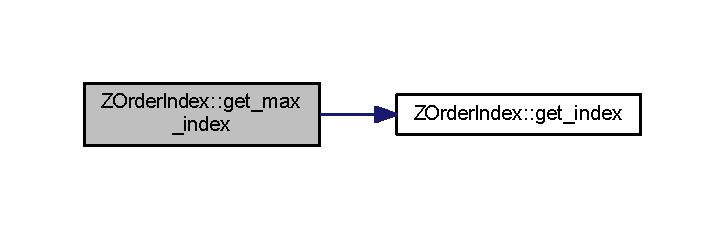
\includegraphics[width=348pt]{class_z_order_index_ac9eacf3a0481b0b26e2b98216c04689e_cgraph}
\end{center}
\end{figure}


\index{Z\-Order\-Index@{Z\-Order\-Index}!get\-\_\-origin\-\_\-index@{get\-\_\-origin\-\_\-index}}
\index{get\-\_\-origin\-\_\-index@{get\-\_\-origin\-\_\-index}!ZOrderIndex@{Z\-Order\-Index}}
\subsubsection[{get\-\_\-origin\-\_\-index}]{\setlength{\rightskip}{0pt plus 5cm}virtual {\bf Row\-Major\-Point} Z\-Order\-Index\-::get\-\_\-origin\-\_\-index (
\begin{DoxyParamCaption}
\item[{{\bf Index\-Type}}]{index}
\end{DoxyParamCaption}
) const\hspace{0.3cm}{\ttfamily [inline]}, {\ttfamily [virtual]}}\label{class_z_order_index_a90fb65a322a8b1f28f3a7e3b0ba5fe27}


get the original row-\/major index 


\begin{DoxyParams}{参数}
{\em index} & the index calculated from \doxyref{get\-\_\-index()}{p.}{class_z_order_index_a12b02aba625065238dc1b5789440d9fa} method \\
\hline
\end{DoxyParams}
\begin{DoxyReturn}{返回}
the row-\/major index (row, col) format 
\end{DoxyReturn}


实现了 {\bf Index\-Method\-Interface} \doxyref{}{p.}{class_index_method_interface_a44f4553bd06c787d4523c37a9a15fdd3}.



在文件 {\bf Index\-Method.\-hpp} 第  行定义.

\index{Z\-Order\-Index@{Z\-Order\-Index}!get\-\_\-row\-\_\-result@{get\-\_\-row\-\_\-result}}
\index{get\-\_\-row\-\_\-result@{get\-\_\-row\-\_\-result}!ZOrderIndex@{Z\-Order\-Index}}
\subsubsection[{get\-\_\-row\-\_\-result}]{\setlength{\rightskip}{0pt plus 5cm}virtual {\bf Index\-Type} Z\-Order\-Index\-::get\-\_\-row\-\_\-result (
\begin{DoxyParamCaption}
\item[{{\bf Row\-Major\-Index\-Type}}]{row\-\_\-index}
\end{DoxyParamCaption}
) const\hspace{0.3cm}{\ttfamily [inline]}, {\ttfamily [virtual]}}\label{class_z_order_index_ae6448044c3c190826a85c29eac950b86}


get the row result from just the row index (for using row-\/major like loop). 


\begin{DoxyPre}
Using this method for some kind of optimization when using row-major like loop 
for example:    
for(size\_t row = 0; row < rows; ++row) \{ 
        IndexType row\_result = get\_row\_result(row);
        for(size\_t col = 0; col < cols; ++col) \{ 
                IndexType index = get\_index\_by\_row\_result(row\_result, col); 
        \} 
\} 
\end{DoxyPre}



\begin{DoxyParams}{参数}
{\em row\-\_\-index} & the index of row in the row-\/major format \\
\hline
\end{DoxyParams}
\begin{DoxyReturn}{返回}
the row result 
\end{DoxyReturn}


实现了 {\bf Index\-Method\-Interface} \doxyref{}{p.}{class_index_method_interface_aab87157a6dcd40f8d249616829f7ec97}.



在文件 {\bf Index\-Method.\-hpp} 第  行定义.



该类的文档由以下文件生成\-:\begin{DoxyCompactItemize}
\item 
D\-:/\-Out\-\_\-\-Of\-\_\-\-Core\-\_\-\-Git/src/Index\-Method.\-hpp\end{DoxyCompactItemize}

\section{Z\-Order\-Index\-Intuition类 参考}
\label{class_z_order_index_intuition}\index{Z\-Order\-Index\-Intuition@{Z\-Order\-Index\-Intuition}}


类 Z\-Order\-Index\-Intuition 继承关系图\-:\nopagebreak
\begin{figure}[H]
\begin{center}
\leavevmode
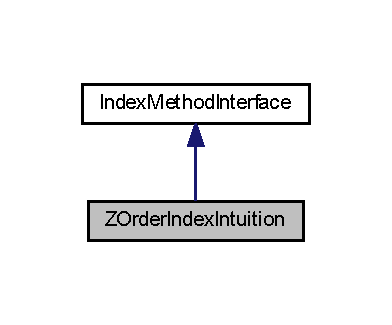
\includegraphics[width=188pt]{class_z_order_index_intuition__inherit__graph}
\end{center}
\end{figure}


Z\-Order\-Index\-Intuition 的协作图\-:\nopagebreak
\begin{figure}[H]
\begin{center}
\leavevmode
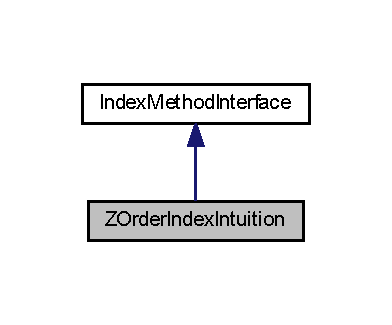
\includegraphics[width=188pt]{class_z_order_index_intuition__coll__graph}
\end{center}
\end{figure}
\subsection*{Public 成员函数}
\begin{DoxyCompactItemize}
\item 
{\bf Z\-Order\-Index\-Intuition} ({\bf Row\-Major\-Index\-Type} row\-\_\-size, {\bf Row\-Major\-Index\-Type} col\-\_\-size)
\item 
virtual {\bf Index\-Type} {\bf get\-\_\-row\-\_\-result} ({\bf Row\-Major\-Index\-Type} row\-\_\-index) const 
\begin{DoxyCompactList}\small\item\em get the row result from just the row index (for using row-\/major like loop). \end{DoxyCompactList}\item 
virtual {\bf Index\-Type} {\bf get\-\_\-index\-\_\-by\-\_\-row\-\_\-result} ({\bf Index\-Type} row\-\_\-result, {\bf Row\-Major\-Index\-Type} col\-\_\-index) const 
\begin{DoxyCompactList}\small\item\em get the index from row result and col index \end{DoxyCompactList}\item 
virtual {\bf Index\-Type} {\bf get\-\_\-index} ({\bf Row\-Major\-Index\-Type} row\-\_\-index, {\bf Row\-Major\-Index\-Type} col\-\_\-index) const \label{class_z_order_index_intuition_a63f6a17ea21fa44cf0a5ed7887b2a572}

\begin{DoxyCompactList}\small\item\em get the index of row-\/major index (row, col) \end{DoxyCompactList}\item 
virtual {\bf Row\-Major\-Point} {\bf get\-\_\-origin\-\_\-index} ({\bf Index\-Type} index) const 
\begin{DoxyCompactList}\small\item\em get the original row-\/major index \end{DoxyCompactList}\item 
virtual {\bf Index\-Type} {\bf get\-\_\-max\-\_\-index} () const 
\begin{DoxyCompactList}\small\item\em get the maximum index, often used to ensure the size of the container \end{DoxyCompactList}\item 
virtual std\-::string {\bf get\-\_\-index\-\_\-method\-\_\-name} () const \label{class_z_order_index_intuition_ac3df90bc072be9be5be2b517885b9ddd}

\begin{DoxyCompactList}\small\item\em get the index method name for identify different method \end{DoxyCompactList}\end{DoxyCompactItemize}
\subsection*{额外继承的成员函数}


\subsection{详细描述}


在文件 {\bf Index\-Method.\-hpp} 第  行定义.



\subsection{构造及析构函数说明}
\index{Z\-Order\-Index\-Intuition@{Z\-Order\-Index\-Intuition}!Z\-Order\-Index\-Intuition@{Z\-Order\-Index\-Intuition}}
\index{Z\-Order\-Index\-Intuition@{Z\-Order\-Index\-Intuition}!ZOrderIndexIntuition@{Z\-Order\-Index\-Intuition}}
\subsubsection[{Z\-Order\-Index\-Intuition}]{\setlength{\rightskip}{0pt plus 5cm}Z\-Order\-Index\-Intuition\-::\-Z\-Order\-Index\-Intuition (
\begin{DoxyParamCaption}
\item[{{\bf Row\-Major\-Index\-Type}}]{row\-\_\-size, }
\item[{{\bf Row\-Major\-Index\-Type}}]{col\-\_\-size}
\end{DoxyParamCaption}
)\hspace{0.3cm}{\ttfamily [inline]}}\label{class_z_order_index_intuition_a048353c02ef1c4858f4c8497de139518}

\begin{DoxyParams}{参数}
{\em row\-\_\-size} & the row size of the image \\
\hline
{\em col\-\_\-size} & the col size of the image \\
\hline
\end{DoxyParams}


在文件 {\bf Index\-Method.\-hpp} 第  行定义.



\subsection{成员函数说明}
\index{Z\-Order\-Index\-Intuition@{Z\-Order\-Index\-Intuition}!get\-\_\-index\-\_\-by\-\_\-row\-\_\-result@{get\-\_\-index\-\_\-by\-\_\-row\-\_\-result}}
\index{get\-\_\-index\-\_\-by\-\_\-row\-\_\-result@{get\-\_\-index\-\_\-by\-\_\-row\-\_\-result}!ZOrderIndexIntuition@{Z\-Order\-Index\-Intuition}}
\subsubsection[{get\-\_\-index\-\_\-by\-\_\-row\-\_\-result}]{\setlength{\rightskip}{0pt plus 5cm}virtual {\bf Index\-Type} Z\-Order\-Index\-Intuition\-::get\-\_\-index\-\_\-by\-\_\-row\-\_\-result (
\begin{DoxyParamCaption}
\item[{{\bf Index\-Type}}]{row\-\_\-result, }
\item[{{\bf Row\-Major\-Index\-Type}}]{col\-\_\-index}
\end{DoxyParamCaption}
) const\hspace{0.3cm}{\ttfamily [inline]}, {\ttfamily [virtual]}}\label{class_z_order_index_intuition_a260c382c65f156a14993c3035adff46c}


get the index from row result and col index 


\begin{DoxyParams}{参数}
{\em row\-\_\-result} & the result get from the \doxyref{get\-\_\-row\-\_\-result()}{p.}{class_z_order_index_intuition_a681922974bbe3800d01345c9a357238e} method \\
\hline
{\em col\-\_\-index} & the index of col in the row-\/major format \\
\hline
\end{DoxyParams}
\begin{DoxyReturn}{返回}
the index result combined both the row and col 
\end{DoxyReturn}


实现了 {\bf Index\-Method\-Interface} \doxyref{}{p.}{class_index_method_interface_af6fda6db139d00aa3e722fcd20945322}.



在文件 {\bf Index\-Method.\-hpp} 第  行定义.

\index{Z\-Order\-Index\-Intuition@{Z\-Order\-Index\-Intuition}!get\-\_\-max\-\_\-index@{get\-\_\-max\-\_\-index}}
\index{get\-\_\-max\-\_\-index@{get\-\_\-max\-\_\-index}!ZOrderIndexIntuition@{Z\-Order\-Index\-Intuition}}
\subsubsection[{get\-\_\-max\-\_\-index}]{\setlength{\rightskip}{0pt plus 5cm}virtual {\bf Index\-Type} Z\-Order\-Index\-Intuition\-::get\-\_\-max\-\_\-index (
\begin{DoxyParamCaption}
{}
\end{DoxyParamCaption}
) const\hspace{0.3cm}{\ttfamily [inline]}, {\ttfamily [virtual]}}\label{class_z_order_index_intuition_aaf09fc4e8668b254e8d8fb0abcc26719}


get the maximum index, often used to ensure the size of the container 

\begin{DoxyReturn}{返回}
the maximum index get from the this indexing method 
\end{DoxyReturn}


实现了 {\bf Index\-Method\-Interface} \doxyref{}{p.}{class_index_method_interface_ad2e684fc1ef5ea505ccbc23278977478}.



在文件 {\bf Index\-Method.\-hpp} 第  行定义.



函数调用图\-:\nopagebreak
\begin{figure}[H]
\begin{center}
\leavevmode
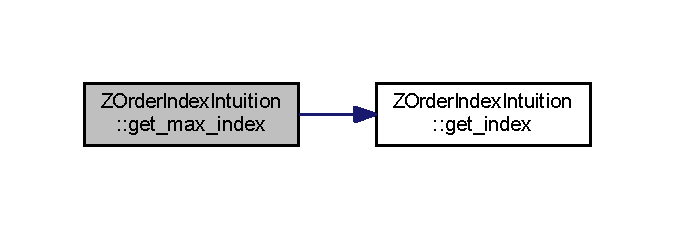
\includegraphics[width=324pt]{class_z_order_index_intuition_aaf09fc4e8668b254e8d8fb0abcc26719_cgraph}
\end{center}
\end{figure}


\index{Z\-Order\-Index\-Intuition@{Z\-Order\-Index\-Intuition}!get\-\_\-origin\-\_\-index@{get\-\_\-origin\-\_\-index}}
\index{get\-\_\-origin\-\_\-index@{get\-\_\-origin\-\_\-index}!ZOrderIndexIntuition@{Z\-Order\-Index\-Intuition}}
\subsubsection[{get\-\_\-origin\-\_\-index}]{\setlength{\rightskip}{0pt plus 5cm}virtual {\bf Row\-Major\-Point} Z\-Order\-Index\-Intuition\-::get\-\_\-origin\-\_\-index (
\begin{DoxyParamCaption}
\item[{{\bf Index\-Type}}]{index}
\end{DoxyParamCaption}
) const\hspace{0.3cm}{\ttfamily [inline]}, {\ttfamily [virtual]}}\label{class_z_order_index_intuition_a2cec2d33763c814a1aa638fc755eea68}


get the original row-\/major index 


\begin{DoxyParams}{参数}
{\em index} & the index calculated from \doxyref{get\-\_\-index()}{p.}{class_z_order_index_intuition_a63f6a17ea21fa44cf0a5ed7887b2a572} method \\
\hline
\end{DoxyParams}
\begin{DoxyReturn}{返回}
the row-\/major index (row, col) format 
\end{DoxyReturn}


实现了 {\bf Index\-Method\-Interface} \doxyref{}{p.}{class_index_method_interface_a44f4553bd06c787d4523c37a9a15fdd3}.



在文件 {\bf Index\-Method.\-hpp} 第  行定义.

\index{Z\-Order\-Index\-Intuition@{Z\-Order\-Index\-Intuition}!get\-\_\-row\-\_\-result@{get\-\_\-row\-\_\-result}}
\index{get\-\_\-row\-\_\-result@{get\-\_\-row\-\_\-result}!ZOrderIndexIntuition@{Z\-Order\-Index\-Intuition}}
\subsubsection[{get\-\_\-row\-\_\-result}]{\setlength{\rightskip}{0pt plus 5cm}virtual {\bf Index\-Type} Z\-Order\-Index\-Intuition\-::get\-\_\-row\-\_\-result (
\begin{DoxyParamCaption}
\item[{{\bf Row\-Major\-Index\-Type}}]{row\-\_\-index}
\end{DoxyParamCaption}
) const\hspace{0.3cm}{\ttfamily [inline]}, {\ttfamily [virtual]}}\label{class_z_order_index_intuition_a681922974bbe3800d01345c9a357238e}


get the row result from just the row index (for using row-\/major like loop). 


\begin{DoxyPre}
Using this method for some kind of optimization when using row-major like loop 
for example:    
for(size\_t row = 0; row < rows; ++row) \{ 
        IndexType row\_result = get\_row\_result(row);
        for(size\_t col = 0; col < cols; ++col) \{ 
                IndexType index = get\_index\_by\_row\_result(row\_result, col); 
        \} 
\} 
\end{DoxyPre}



\begin{DoxyParams}{参数}
{\em row\-\_\-index} & the index of row in the row-\/major format \\
\hline
\end{DoxyParams}
\begin{DoxyReturn}{返回}
the row result 
\end{DoxyReturn}


实现了 {\bf Index\-Method\-Interface} \doxyref{}{p.}{class_index_method_interface_aab87157a6dcd40f8d249616829f7ec97}.



在文件 {\bf Index\-Method.\-hpp} 第  行定义.



该类的文档由以下文件生成\-:\begin{DoxyCompactItemize}
\item 
D\-:/\-Out\-\_\-\-Of\-\_\-\-Core\-\_\-\-Git/src/Index\-Method.\-hpp\end{DoxyCompactItemize}

\chapter{示例说明}
\section{test\-Image\-Containter.\-cpp}
This an example of how to use the image processing interface in the \doxyref{Blockwise\-Image}{p.}{class_blockwise_image} class.


\begin{DoxyCodeInclude}
\textcolor{preprocessor}{#include <iostream>}
\textcolor{preprocessor}{#include <string>}

\textcolor{preprocessor}{#include <opencv2/core/core.hpp>}
\textcolor{preprocessor}{#include <opencv2/imgproc/imgproc.hpp>}
\textcolor{preprocessor}{#include <opencv2/highgui/highgui.hpp>}

\textcolor{preprocessor}{#include "../src/HierarchicalImage.hpp"}

\textcolor{preprocessor}{#include <boost/assert.hpp>}
\textcolor{preprocessor}{#include <boost/progress.hpp>}
\textcolor{preprocessor}{#include <boost/timer.hpp>}

\textcolor{keyword}{using namespace }std;

\textcolor{keyword}{typedef} GiantImageInterface<Vec3b> BigImageType;
\textcolor{keyword}{typedef} boost::shared\_ptr<BigImageType> BigImagePtr;
\textcolor{keyword}{typedef} DiskBigImage<Vec3b> DiskImageType;
\textcolor{keyword}{typedef} boost::shared\_ptr<DiskImageType> DiskImagePtr;
\textcolor{keyword}{typedef} ZOrderIndex ZOrderIndexType;

\textcolor{keyword}{static} BigImagePtr build\_enlarged\_image(\textcolor{keyword}{const} \textcolor{keywordtype}{char} *file\_name, \textcolor{keywordtype}{size\_t} 
      enlarge\_number, \textcolor{keywordtype}{size\_t} memory\_usage);

BigImagePtr build\_enlarged\_image(\textcolor{keyword}{const} \textcolor{keywordtype}{char} *file\_name, \textcolor{keywordtype}{size\_t} enlarge\_number, \textcolor{keywordtype}{
      size\_t} memory\_usage)
\{
        cv::Mat original\_img = cv::imread(file\_name);
        \textcolor{keywordflow}{if}(original\_img.empty()) \{
                cerr << \textcolor{stringliteral}{"Load image error"} << endl;
                \textcolor{keywordflow}{return} BigImagePtr();
        \}

        BOOST\_ASSERT\_MSG(original\_img.depth() == CV\_8U, \textcolor{stringliteral}{"image depth not
       correct"});
        BOOST\_ASSERT\_MSG(original\_img.channels() == 3, \textcolor{stringliteral}{"image channels not
       correct"});

        \textcolor{keywordtype}{size\_t} rows = original\_img.rows, cols = original\_img.cols;
        \textcolor{keywordtype}{size\_t} large\_rows = rows * enlarge\_number, large\_cols = cols * 
      enlarge\_number;

        boost::shared\_ptr<IndexMethodInterface> index\_method = 
      boost::make\_shared<ZOrderIndex>(large\_rows, large\_cols);
        \textcolor{comment}{//init the config file}
        \{
                \textcolor{keywordtype}{size\_t} imageBytes = (double)(index\_method->get\_max\_index() * \textcolor{keyword}{
      sizeof}(Vec3b)) / (1024*1024);
                fstream fout(\textcolor{stringliteral}{"config.stxxl"}, ios::out | ios::trunc);
                fout << \textcolor{stringliteral}{"disk=d:\(\backslash\)\(\backslash\)stxxl,"} << (imageBytes * 2) <<\textcolor{stringliteral}{",wincall"} << 
      endl;
                fout.close();
        \}

        \textcolor{comment}{//the container to store the enlarged image}
        BigImagePtr p\_big\_image = get\_block\_wise\_image\_by\_meomory\_usage<Vec3b>(
      memory\_usage, large\_rows, large\_cols, 1, 1, index\_method);
        BigImageType &big\_image = *p\_big\_image;
        big\_image.set\_file\_node\_size(1024*1024);

        \textcolor{comment}{//time related}
        boost::progress\_display pd(enlarge\_number*enlarge\_number);
        boost::timer t;
        t.restart();

        \textcolor{comment}{//the ZOrder part}
        \textcolor{keyword}{typedef} ZOrderIndexType::IndexType IndexType;
        \textcolor{keywordflow}{for}(IndexType outI = 0; outI < enlarge\_number; ++outI) \{
                \textcolor{keywordflow}{for}(IndexType outJ = 0; outJ < enlarge\_number; ++outJ) \{
                        IndexType startI = outI * rows;
                        IndexType startJ = outJ * cols;
                        \textcolor{keywordflow}{for}(IndexType i = 0; i < rows; ++i) \{
                                IndexType I = startI + i;
                                \textcolor{keywordflow}{for}(IndexType j = 0; j < cols; ++j) \{
                                        IndexType J = startJ + j;
                                        big\_image(I, J) = *(Vec3b*)(
      original\_img.data + i*original\_img.step[0] + j*original\_img.step[1]);
                                \}
                        \}
                        ++pd;
                \}
        \}
        cout << \textcolor{stringliteral}{"Build Enlarged Image Cost Time : "} << t.elapsed() << \textcolor{stringliteral}{" s "} << 
      endl;

        \textcolor{keywordflow}{return} p\_big\_image;
\}

\textcolor{comment}{/*}
\textcolor{comment}{ * 1) read a picture}
\textcolor{comment}{ * 2) enlarge it to get a big image (test the container ability)}
\textcolor{comment}{ * 3) input the range information to get the image range data }
\textcolor{comment}{ */}
\textcolor{keywordtype}{bool} test\_big\_image\_containter(\textcolor{keywordtype}{int} argc, \textcolor{keywordtype}{char} **argv)
\{
        \textcolor{keywordflow}{if}(argc < 5) \{
                cout << \textcolor{stringliteral}{"Read a image file first, just enlarge the image in
       both hierarchical and vertical "} << endl
                        << \textcolor{stringliteral}{"Para : enlarge number (the enlarge number of image
       in both hierarchical and vertical)"} << endl
                        << \textcolor{stringliteral}{"Para : memory usage (the maximum memory can be
       used)"} << endl
                        << \textcolor{stringliteral}{"Para : show image (whether show the enlarged image,
       too large is forbidden)"} << endl;

                cout << \textcolor{stringliteral}{"Usage : "} << \textcolor{stringliteral}{"[fileName] [enlarge number] [resRow]
       [resCol] "}
                        \textcolor{stringliteral}{"[memory usage(optional)] [show image(optional)]"} << 
      endl;
                \textcolor{keywordflow}{return} \textcolor{keyword}{false};
        \}

        \textcolor{keyword}{const} \textcolor{keywordtype}{char} *file\_name = argv[1];
        \textcolor{keywordtype}{size\_t} enlarge\_number = atoi(argv[2]);
        \textcolor{keyword}{const} \textcolor{keywordtype}{int} res\_row = atoi(argv[3]);
        \textcolor{keyword}{const} \textcolor{keywordtype}{int} res\_col = atoi(argv[4]);
        \textcolor{keywordtype}{size\_t} memory\_usage = (argc >= 6) ? (atoi(argv[5])) : 64;
        \textcolor{keywordtype}{bool} bShowImg = (argc >= 7 && (string(argv[6]) == \textcolor{stringliteral}{"1"} || string(argv[6]
      ) == \textcolor{stringliteral}{"true"})) ? \textcolor{keyword}{true} : \textcolor{keyword}{false};

        BigImagePtr p\_big\_image = build\_enlarged\_image(file\_name, 
      enlarge\_number, memory\_usage);
        \textcolor{keywordflow}{if}(!p\_big\_image) \textcolor{keywordflow}{return} \textcolor{keyword}{false};
        BigImageType &big\_image = *p\_big\_image;

        \textcolor{keywordtype}{size\_t} large\_rows = big\_image.get\_image\_rows(), large\_cols = big\_image.
      get\_image\_cols();
        \textcolor{keywordflow}{if}(bShowImg)
        \{
                boost::timer t;

                std::vector<Vec3b> data;
                \textcolor{keywordflow}{try} \{

            big\_image.get\_pixels(0, 0, big\_image.get\_image\_rows(), big\_image.
      get\_image\_cols(), data);

            cout << \textcolor{stringliteral}{"get the all data from zorder based container "} << t.
      elapsed() << \textcolor{stringliteral}{" s "} << endl;

            cv::Mat result\_image(large\_rows, large\_cols, CV\_8UC3, data.data());
            cv::namedWindow(\textcolor{stringliteral}{"Enlarged Image"});
            cv::imshow(\textcolor{stringliteral}{"Enlarged Image"}, result\_image);
            cv::waitKey(0);

                \} \textcolor{keywordflow}{catch} (std::exception &err) \{
                        cerr << err.what() << endl;
                        \textcolor{keywordflow}{return} \textcolor{keyword}{false};
                \}
        \}

        cout << \textcolor{stringliteral}{"Large Image Size Is : ("} << large\_rows << \textcolor{stringliteral}{","} << large\_cols <<
       \textcolor{stringliteral}{")"} << endl;

        \textcolor{comment}{/* save the input para */}
        std::string str\_array[4];
        \textcolor{keywordflow}{while}(1) \{
                cout << \textcolor{stringliteral}{"Input (quit to exit) : [start\_row] [start\_col] [rows]
       [cols]"} << endl;

                cin >> str\_array[0];
                \textcolor{keywordflow}{if}(str\_array[0] == \textcolor{stringliteral}{"quit"})      \textcolor{keywordflow}{return} \textcolor{keyword}{true};

                cin >> str\_array[1] >> str\_array[2] >> str\_array[3];

                \textcolor{keywordtype}{int} start\_row = atoi(str\_array[0].c\_str());
                \textcolor{keywordtype}{int} start\_col = atoi(str\_array[1].c\_str());
                \textcolor{keywordtype}{int} rows = atoi(str\_array[2].c\_str());
                \textcolor{keywordtype}{int} cols = atoi(str\_array[3].c\_str());

                \textcolor{keywordflow}{try}\{
                        std::vector<Vec3b> vec;
                        \textcolor{keywordflow}{if}(!big\_image.get\_pixels(start\_row, start\_col, rows, 
      cols, vec))
                                \textcolor{keywordflow}{continue};

                        cv::Mat result\_image(rows, cols, CV\_8UC3, vec.data());
                        cv::namedWindow(\textcolor{stringliteral}{"RangeArea"});
                        cv::imshow(\textcolor{stringliteral}{"RangeArea"}, result\_image);
                        cv::waitKey(2000);

                \} \textcolor{keywordflow}{catch}(std::exception &err) \{
                        cout << err.what() << endl;
                        \textcolor{keywordflow}{return} \textcolor{keyword}{false};
                \}
        \}

        \textcolor{keywordflow}{return} \textcolor{keyword}{true};
\}
\end{DoxyCodeInclude}
 
\section{test\-Index\-Method.\-cpp}
This an example of how to use the index method.


\begin{DoxyCodeInclude}
\textcolor{preprocessor}{#include <iostream>}
\textcolor{preprocessor}{#include <iomanip>}
\textcolor{preprocessor}{#include <algorithm>}
\textcolor{preprocessor}{#include <vector>}
\textcolor{preprocessor}{#include <boost/assert.hpp>}
\textcolor{preprocessor}{#include <string>}

\textcolor{preprocessor}{#include "../src/IndexMethod.hpp"}

\textcolor{keyword}{using namespace }std;

\textcolor{comment}{/* test the block index method, input the rows, cols, blockrows, blockcols for
       testing */}
\textcolor{keywordtype}{bool} test\_block\_index(\textcolor{keywordtype}{int} argc, \textcolor{keywordtype}{char} **argv)
\{
        \textcolor{keywordflow}{if}(argc < 5) \{
                cout << \textcolor{stringliteral}{"Usage : [row count] [col count] [block row size n(by
       2^n)] [block col size n(by 2^n)]"} << endl;
                \textcolor{keywordflow}{return} \textcolor{keyword}{false};
        \}

        \textcolor{keyword}{typedef} Block2DIndex::IndexType IndexType;
        \textcolor{keyword}{typedef} Block2DIndex::RowMajorIndexType RowMajorType;

        IndexType rowCount = atoi(argv[1]);
        IndexType colCount = atoi(argv[2]);
        IndexType blockRowOrderSize = atoi(argv[3]);
        IndexType blockColOrderSize = atoi(argv[4]);

        Block2DIndex blockObject(rowCount, colCount, blockRowOrderSize, 
      blockColOrderSize);

        \{
                cout << \textcolor{stringliteral}{"method one : using get\_index method : "} << endl;
                cout << \textcolor{stringliteral}{"
      *******************************************************"} << endl;
                IndexType totalSize = blockObject.get_max_index();
                \textcolor{keywordtype}{int} *vec = \textcolor{keyword}{new} \textcolor{keywordtype}{int}[totalSize];
                std::generate(vec, vec + totalSize, []()->\textcolor{keywordtype}{int} \{
                        \textcolor{keywordflow}{return} -1;
                \});

                \textcolor{keywordflow}{for}(RowMajorType i = 0; i < rowCount; ++i) \{
                        \textcolor{keywordflow}{for}(RowMajorType j = 0; j < colCount; ++j) \{
                                vec[blockObject.get_index(i, j)] = i*colCount +
       j;
                        \}
                \}

                IndexType blockSize = blockObject.getBlockTotalSize();

                IndexType blockColSize = blockObject.getBlockColSize();
                IndexType blockIndex = 0;

                cout << \textcolor{stringliteral}{"the after block : "} << endl;
                cout << \textcolor{stringliteral}{"------------------------------------------------------
      "} << endl;
                \textcolor{keywordflow}{for}(IndexType index = 0; index < totalSize;) \{
                        cout << setw(8) << vec[index++];

                        \textcolor{comment}{//meet the end of the small block line}
                        \textcolor{keywordflow}{if}(index % blockColSize == 0) cout << endl;

                        \textcolor{keywordflow}{if}(index % blockSize == 0) cout << \textcolor{stringliteral}{"
      ------------------------------------------------------"} << endl;
                \}
                cout << endl;

                cout << \textcolor{stringliteral}{"get row major index : "} << endl;
                cout << \textcolor{stringliteral}{"------------------------------------------------------
      "} << endl;
                \textcolor{keywordflow}{for}(IndexType index = 0; index < totalSize;) \{
                        RowMajorPoint point = blockObject.get_origin_index(
      index++);
                        cout << setw(8) << \textcolor{stringliteral}{"("} << point.row << \textcolor{stringliteral}{","} << point.col
       << \textcolor{stringliteral}{")"};
                        \textcolor{keywordflow}{if}(index % blockColSize == 0) cout << endl;
                        \textcolor{keywordflow}{if}(index % blockSize == 0) cout << \textcolor{stringliteral}{"
      ------------------------------------------------------"} << endl;
                \}
                cout << endl;
        \}

        \{
                cout << \textcolor{stringliteral}{"method two : using get\_index\_by\_row\_index method : "} <
      < endl;
                cout << \textcolor{stringliteral}{"
      *******************************************************"} << endl;
                IndexType totalSize = blockObject.get_max_index();
                \textcolor{keywordtype}{int} *vec = \textcolor{keyword}{new} \textcolor{keywordtype}{int}[totalSize];
                std::generate(vec, vec + totalSize, []()->\textcolor{keywordtype}{int} \{
                        \textcolor{keywordflow}{return} -1;
                \});

                \textcolor{keywordflow}{for}(RowMajorType i = 0; i < rowCount; ++i) \{
                        IndexType row\_result = blockObject.get_row_result(i);
                        \textcolor{keywordflow}{for}(RowMajorType j = 0; j < colCount; ++j) \{
                                vec[blockObject.get_index_by_row_result(
      row\_result, j)] = i*colCount + j;
                        \}
                \}

                IndexType blockSize = blockObject.getBlockTotalSize();

                IndexType blockColSize = blockObject.getBlockColSize();
                IndexType blockIndex = 0;

                cout << \textcolor{stringliteral}{"the after block : "} << endl;
                cout << \textcolor{stringliteral}{"------------------------------------------------------
      "} << endl;
                \textcolor{keywordflow}{for}(IndexType index = 0; index < totalSize;) \{
                        cout << setw(8) << vec[index++];

                        \textcolor{comment}{//meet the end of the small block line}
                        \textcolor{keywordflow}{if}(index % blockColSize == 0) cout << endl;

                        \textcolor{keywordflow}{if}(index % blockSize == 0) cout << \textcolor{stringliteral}{"
      ------------------------------------------------------"} << endl;
                \}
                cout << endl;

                cout << \textcolor{stringliteral}{"get row major index : "} << endl;
                cout << \textcolor{stringliteral}{"------------------------------------------------------
      "} << endl;
                \textcolor{keywordflow}{for}(IndexType index = 0; index < totalSize;) \{
                        RowMajorPoint point = blockObject.get_origin_index(
      index++);
                        cout << setw(8) << \textcolor{stringliteral}{"("} << point.row << \textcolor{stringliteral}{","} << point.col
       << \textcolor{stringliteral}{")"};
                        \textcolor{keywordflow}{if}(index % blockColSize == 0) cout << endl;
                        \textcolor{keywordflow}{if}(index % blockSize == 0) cout << \textcolor{stringliteral}{"
      ------------------------------------------------------"} << endl;
                \}
                cout << endl;
        \}
        \textcolor{keywordflow}{return} \textcolor{keyword}{true};
\}
\textcolor{keyword}{template}<\textcolor{keyword}{typename} T, \textcolor{keyword}{typename} RowMajorType>
\textcolor{keywordtype}{void} printTwoArrayVector(T array, RowMajorType row, RowMajorType col, \textcolor{keywordtype}{string} 
      arrayInfo = \textcolor{stringliteral}{""}, ostream& os = cout) \{
        os << arrayInfo << endl;
        \textcolor{keywordflow}{for}(RowMajorType i = 0; i < row; ++i) \{
                \textcolor{keywordflow}{for}(RowMajorType j = 0; j < col; ++j) \{
                        os << setw(8) << array[i*col + j];
                \}
                os << endl;
        \}
        os << endl;
\}

\textcolor{comment}{/* test zorder index, input the rows and cols for indexing */}
\textcolor{keyword}{typedef} ZOrderIndex ZOrderIndexType;
\textcolor{keywordtype}{bool} test\_zorder\_index(\textcolor{keywordtype}{int} argc, \textcolor{keywordtype}{char} **argv)
\{
        \textcolor{keywordflow}{if}(argc < 3) \{
                cout << \textcolor{stringliteral}{"Usage : [row] [col] "} << endl;
                \textcolor{keywordflow}{return} \textcolor{keyword}{false};
        \}

        \textcolor{keywordtype}{size\_t} row = atoi(argv[1]);
        \textcolor{keywordtype}{size\_t} col = atoi(argv[2]);

        \textcolor{comment}{//just insure the row and col are even}
        \textcolor{comment}{//BOOST\_ASSERT((row & 1) == 0 && (col & 1) == 0);}

        \textcolor{keyword}{typedef} std::vector<int> VecType;
        \textcolor{keyword}{typedef} ZOrderIndexType::IndexType IndexType;

        cout << \textcolor{stringliteral}{"method one : using get\_index method : "} << endl;
        cout << \textcolor{stringliteral}{"*******************************************************"} << 
      endl;
        \{
                \textcolor{comment}{//save the original data}
                VecType vec(row * col);
                \textcolor{keywordflow}{for}(IndexType i = 0; i < vec.size(); ++i) vec[i] = i;

                ZOrderIndexType zorder(row, col);
                \textcolor{comment}{//the after Z-order index data}
                IndexType maxIndex = zorder.get\_max\_index();
                VecType newVec(maxIndex + 1);

                IndexType result, rowResult;
                cout << \textcolor{stringliteral}{"zorder index result"} << endl;
                \textcolor{keywordflow}{for}(\textcolor{keywordtype}{size\_t} i = 0; i < row; ++i) \{
                        rowResult = zorder.get\_row\_result(i);
                        \textcolor{keywordflow}{for}(\textcolor{keywordtype}{size\_t} j = 0; j < col; ++j) \{
                                result = zorder.get\_index\_by\_row\_result(
      rowResult, j);
                                cout << setw(8) << result;

                                newVec[result] = vec[i*col + j];
                        \} \textcolor{comment}{//end for of col}
                        cout << endl;
                \} \textcolor{comment}{// end for of row}

                printTwoArrayVector(newVec, row, col, \textcolor{stringliteral}{"zorder index array"});

                VecType testVec(col * row);
                \textcolor{keywordflow}{for}(IndexType i = 0; i < newVec.size(); ++i) \{
                        RowMajorPoint point = zorder.get\_origin\_index(i);
                        \textcolor{keywordtype}{size\_t} x = point.row;
                        \textcolor{keywordtype}{size\_t} y = point.col;
                        \textcolor{keywordflow}{if}(x < row && y < col) testVec[x*col + y] = newVec[i];
                \}

                printTwoArrayVector(testVec, row, col, \textcolor{stringliteral}{"get back vector"});

                \textcolor{keywordflow}{if}(std::equal(vec.begin(), vec.end(), testVec.begin()))
                        cout << \textcolor{stringliteral}{"the result is correct"} << endl;
                \textcolor{keywordflow}{else}
                        cout << \textcolor{stringliteral}{"the result is not correct"} << endl;
        \}

        cout << \textcolor{stringliteral}{"method two : using get\_index\_by\_row\_index method : "} << endl;
        cout << \textcolor{stringliteral}{"*******************************************************"} << 
      endl;
        \{
                \textcolor{comment}{//save the original data}
                VecType vec(row * col);
                \textcolor{keywordflow}{for}(IndexType i = 0; i < vec.size(); ++i) vec[i] = i;

                ZOrderIndexType zorder(row, col);
                \textcolor{comment}{//the after Z-order index data}
                IndexType maxIndex = zorder.get\_max\_index();
                VecType newVec(maxIndex + 1);

                IndexType result, rowResult;
                cout << \textcolor{stringliteral}{"zorder index result"} << endl;
                \textcolor{keywordflow}{for}(\textcolor{keywordtype}{size\_t} i = 0; i < row; ++i) \{
                        \textcolor{keywordflow}{for}(\textcolor{keywordtype}{size\_t} j = 0; j < col; ++j) \{
                                result = zorder.get\_index(i, j);
                                cout << setw(8) << result;

                                newVec[result] = vec[i*col + j];
                        \} \textcolor{comment}{//end for of col}
                        cout << endl;
                \} \textcolor{comment}{// end for of row}

                printTwoArrayVector(newVec, row, col, \textcolor{stringliteral}{"zorder index array"});

                VecType testVec(col * row);
                \textcolor{keywordflow}{for}(IndexType i = 0; i < newVec.size(); ++i) \{
                        RowMajorPoint point = zorder.get\_origin\_index(i);
                        \textcolor{keywordtype}{size\_t} x = point.row;
                        \textcolor{keywordtype}{size\_t} y = point.col;
                        \textcolor{keywordflow}{if}(x < row && y < col) testVec[x*col + y] = newVec[i];
                \}

                printTwoArrayVector(testVec, row, col, \textcolor{stringliteral}{"get back vector"});

                \textcolor{keywordflow}{if}(std::equal(vec.begin(), vec.end(), testVec.begin()))
                        cout << \textcolor{stringliteral}{"the result is correct"} << endl;
                \textcolor{keywordflow}{else}
                        cout << \textcolor{stringliteral}{"the result is not correct"} << endl;
        \}

        \textcolor{keywordflow}{return} \textcolor{keyword}{true};
\}
\end{DoxyCodeInclude}
 
\section{test\-Reading\-Disk\-Image.\-cpp}
Showing how to use the \doxyref{Disk\-Big\-Image}{p.}{class_disk_big_image} class. This an example of how to read the image data from the big image that stored in the file system.


\begin{DoxyCodeInclude}
\textcolor{preprocessor}{#include "../src/DiskBigImage.hpp"}

\textcolor{preprocessor}{#include <opencv2/core/core.hpp>}
\textcolor{preprocessor}{#include <opencv2/highgui/highgui.hpp>}
\textcolor{preprocessor}{#include <opencv2/imgproc/imgproc.hpp>}

\textcolor{preprocessor}{#include <iostream>}
\textcolor{preprocessor}{#include <string>}

\textcolor{comment}{/*}
\textcolor{comment}{ * test the correctness of reading a big image from disk that was wrote by
       BlockwiseImage or HierarchicalImage}
\textcolor{comment}{ * input the (*.bigimage) file name, then get the range image data}
\textcolor{comment}{ */}

\textcolor{keywordtype}{bool} test\_read\_level\_range\_image(\textcolor{keywordtype}{int} argc, \textcolor{keywordtype}{char} **argv)
\{
        \textcolor{keyword}{using namespace }std;
        \textcolor{keywordflow}{if}(argc < 2) \{
                cout << \textcolor{stringliteral}{"Input the big image file name to get level data"} << 
      endl;
                cout << \textcolor{stringliteral}{"Usage : [image file name] "} << endl;
                \textcolor{keywordflow}{return} \textcolor{keyword}{false};
        \}

        \textcolor{keyword}{const} \textcolor{keywordtype}{char} *file\_name = argv[1];
        boost::shared\_ptr<DiskBigImageInterface<Vec3b> > big\_image = 
      load\_disk\_image<Vec3b>(file\_name); 
        \textcolor{keywordflow}{if}(!big\_image) \{
                cerr << \textcolor{stringliteral}{"can't load image "} << endl;
                \textcolor{keywordflow}{return} \textcolor{keyword}{false};
        \}

        \textcolor{comment}{/* save the input para */}
        std::string str\_array[5];
        \textcolor{keywordflow}{while}(1) \{
                cout << \textcolor{stringliteral}{"Input (quit to exit) : [image level] [start\_row]
       [start\_col] [rows] [cols]"} << endl;

                cin >> str\_array[0];
                \textcolor{keywordflow}{if}(str\_array[0] == \textcolor{stringliteral}{"quit"})      \textcolor{keywordflow}{return} \textcolor{keyword}{true};

                cin >> str\_array[1] >> str\_array[2] >> str\_array[3] >> 
      str\_array[4];

                \textcolor{keywordtype}{int} level = atoi(str\_array[0].c\_str());
                \textcolor{keywordtype}{int} start\_row = atoi(str\_array[1].c\_str());
                \textcolor{keywordtype}{int} start\_col = atoi(str\_array[2].c\_str());
                \textcolor{keywordtype}{int} rows = atoi(str\_array[3].c\_str());
                \textcolor{keywordtype}{int} cols = atoi(str\_array[4].c\_str());

                \textcolor{keywordflow}{if}(!big\_image->set\_current\_level(level)) \textcolor{keywordflow}{continue};

                cout << \textcolor{stringliteral}{"The level image size is "} << \textcolor{stringliteral}{"("}
                        << big\_image->get\_current\_level\_image\_rows() << \textcolor{stringliteral}{","} 
                        << big\_image->get\_current\_level\_image\_cols() << \textcolor{stringliteral}{")"} << 
      endl;

                \textcolor{keywordflow}{try}\{
                        std::vector<Vec3b> vec;
                        \textcolor{keywordflow}{if}(!big\_image->get\_pixels\_by\_level(level, start\_row, 
      start\_col, rows, cols, vec))
                                \textcolor{keywordflow}{continue};

                        cv::Mat result\_image(rows, cols, CV\_8UC3, vec.data());

                        \textcolor{comment}{/* image data was wrote in the format of RGB, but
       opencv is BRG*/}
                        cv::cvtColor(result\_image, result\_image, CV\_RGB2BGR);
                        cv::namedWindow(\textcolor{stringliteral}{"get pixel by level image"});
                        cv::imshow(\textcolor{stringliteral}{"get pixel by level image"}, result\_image);
                        cv::waitKey(2000);

                \} \textcolor{keywordflow}{catch}(std::exception &err) \{
                        cout << err.what() << endl;
                        \textcolor{keywordflow}{return} \textcolor{keyword}{false};
                \}
        \}

        \textcolor{keywordflow}{return} \textcolor{keyword}{true};
\}
\end{DoxyCodeInclude}
 
\section{Write\-Block\-Wise\-Image.\-cpp}
This an example of how to write the block wise image into the file system.


\begin{DoxyCodeInclude}
\textcolor{comment}{// WriteBlockWiseImage.cpp : Defines the entry point for the console
       application.}
\textcolor{comment}{//}

\textcolor{preprocessor}{#include "../src/BlockwiseImage.hpp"}

\textcolor{preprocessor}{#include <boost/timer.hpp>}
\textcolor{preprocessor}{#include <boost/progress.hpp>}

\textcolor{comment}{/* opencv part */}
\textcolor{preprocessor}{#include <opencv2/core/core.hpp>}
\textcolor{preprocessor}{#include <opencv2/highgui/highgui.hpp>}
\textcolor{preprocessor}{#include <opencv2/imgproc/imgproc.hpp>}

\textcolor{preprocessor}{#ifdef NDEBUG}
\textcolor{preprocessor}{}\textcolor{preprocessor}{#pragma comment(lib, "opencv\_highgui240.lib")}
\textcolor{preprocessor}{}\textcolor{preprocessor}{#pragma comment(lib, "opencv\_core240.lib")}
\textcolor{preprocessor}{}\textcolor{preprocessor}{#pragma comment(lib, "opencv\_imgproc240.lib")}
\textcolor{preprocessor}{}\textcolor{preprocessor}{#else}
\textcolor{preprocessor}{}\textcolor{preprocessor}{#pragma comment(lib, "opencv\_highgui240d.lib")}
\textcolor{preprocessor}{}\textcolor{preprocessor}{#pragma comment(lib, "opencv\_core240d.lib")}
\textcolor{preprocessor}{}\textcolor{preprocessor}{#pragma comment(lib, "opencv\_imgproc240d.lib")}
\textcolor{preprocessor}{}\textcolor{preprocessor}{#endif}
\textcolor{preprocessor}{}\textcolor{comment}{/*---------------------------------------------*/}

\textcolor{keywordtype}{bool} test\_writing\_blockwise(\textcolor{keywordtype}{int} argc, \textcolor{keywordtype}{char} **argv)
\{
        \textcolor{keyword}{using namespace }std;

        \textcolor{keywordflow}{if}(argc < 6) \{
                cout << \textcolor{stringliteral}{"Usage : [file name] [res row] [res col] [write image
       file name] [enlarge number]"}
                        \textcolor{stringliteral}{" [optinal (show image)] "} << endl;
                \textcolor{keywordflow}{return} \textcolor{keyword}{false};
        \}

        \textcolor{keyword}{const} \textcolor{keywordtype}{char} *file\_name = argv[1];
        \textcolor{keywordtype}{size\_t} mini\_rows = atoi(argv[2]);
        \textcolor{keywordtype}{size\_t} mini\_cols = atoi(argv[3]);
        \textcolor{keyword}{const} \textcolor{keywordtype}{char} *write\_image\_name = argv[4];
        \textcolor{keywordtype}{size\_t} enlarge\_number = atoi(argv[5]);
        \textcolor{keywordtype}{bool} show\_image = (argc >= 7) ? atoi(argv[6]) : \textcolor{keyword}{false};

        cv::Mat original\_img = cv::imread(file\_name);
        \textcolor{keywordflow}{if}(original\_img.empty()) \{
                cerr << \textcolor{stringliteral}{"Load image error"} << endl;
                \textcolor{keywordflow}{return} \textcolor{keyword}{false};
        \}

        BOOST\_ASSERT\_MSG(original\_img.depth() == CV\_8U, \textcolor{stringliteral}{"image depth not
       correct"});
        BOOST\_ASSERT\_MSG(original\_img.channels() == 3, \textcolor{stringliteral}{"image channels not
       correct"});

        cv::cvtColor(original\_img, original\_img, CV\_BGR2RGB);

        \textcolor{keywordtype}{size\_t} rows = original\_img.rows, cols = original\_img.cols;
        \textcolor{keywordtype}{size\_t} large\_rows = rows * enlarge\_number, large\_cols = cols * 
      enlarge\_number;

        boost::shared\_ptr<IndexMethodInterface> index\_method = 
      boost::make\_shared<ZOrderIndex>(large\_rows, large\_cols);
        \textcolor{comment}{//init the config file}
        \{
                \textcolor{keywordtype}{size\_t} imageBytes = (double)(index\_method->get\_max\_index() * \textcolor{keyword}{
      sizeof}(Vec3b)) / (1024*1024);
                fstream fout(\textcolor{stringliteral}{"config.stxxl"}, ios::out | ios::trunc);
                fout << \textcolor{stringliteral}{"disk=d:\(\backslash\)\(\backslash\)stxxl,"} << (imageBytes * 2) <<\textcolor{stringliteral}{",wincall"} << 
      endl;
                fout.close();
        \}

        \textcolor{keyword}{typedef} BlockwiseImage<Vec3b, 512> ImageType;
        ImageType big\_image(large\_rows, large\_cols, mini\_rows, mini\_cols);
        cout << \textcolor{stringliteral}{"mini\_rows "} << big\_image.get\_minimal\_image\_rows() << endl;
        cout << \textcolor{stringliteral}{"mini\_cols "} << big\_image.get\_minimal\_image\_cols() << endl;
        cout << \textcolor{stringliteral}{"max\_level "} << big\_image.get\_max\_image\_level() << endl;

        \textcolor{comment}{//time related}
        boost::progress\_display pd(enlarge\_number*enlarge\_number);
        boost::timer t;
        t.restart();

        \textcolor{comment}{//the ZOrder part}
        \textcolor{keyword}{typedef} ZOrderIndex::IndexType IndexType;
        \textcolor{keywordflow}{for}(IndexType outI = 0; outI < enlarge\_number; ++outI) \{
                \textcolor{keywordflow}{for}(IndexType outJ = 0; outJ < enlarge\_number; ++outJ) \{
                        IndexType startI = outI * rows;
                        IndexType startJ = outJ * cols;
                        \textcolor{keywordflow}{for}(IndexType i = 0; i < rows; ++i) \{
                                IndexType I = startI + i;
                                \textcolor{keywordflow}{for}(IndexType j = 0; j < cols; ++j) \{
                                        IndexType J = startJ + j;
                                        big\_image(I, J) = *(Vec3b*)(
      original\_img.data + i*original\_img.step[0] + j*original\_img.step[1]);
                                \}
                        \}
                        ++pd;
                \}
        \}
        cout << \textcolor{stringliteral}{"Build Enlarged Image Cost Time : "} << t.elapsed() << \textcolor{stringliteral}{" s "} << 
      endl;

        t.restart();

        \textcolor{comment}{/* 6M per file */}
        big\_image.set\_file\_node\_size(6*1024*1024);

        \textcolor{keywordflow}{if}(!big\_image.write\_image(write\_image\_name)) \textcolor{keywordflow}{return} \textcolor{keyword}{false};
        cout << \textcolor{stringliteral}{"Write Hierarchical Image Cost : "} << t.elapsed() << \textcolor{stringliteral}{" s "} << 
      endl;

        \textcolor{keywordflow}{if}(show\_image) \{
                \textcolor{keyword}{const} ImageType &c\_big\_image = big\_image;
                std::vector<Vec3b> vec(large\_rows*large\_cols);
                \textcolor{keywordflow}{for}(IndexType i = 0; i < big\_image.get\_image\_rows(); ++i) \{
                        \textcolor{keywordflow}{for}(IndexType j = 0; j < big\_image.get\_image\_cols(); ++
      j) \{
                                vec[i*large\_cols  + j] = c\_big\_image(i,j);
                        \}
                \}

                cv::Mat result\_image(large\_rows, large\_cols, CV\_8UC3, vec.data(
      ));
                cv::cvtColor(result\_image, result\_image, CV\_RGB2BGR);
                cv::namedWindow(\textcolor{stringliteral}{"hierarchical image"});
                cv::imshow(\textcolor{stringliteral}{"hierarchical image"}, result\_image);
                cv::waitKey(0);
        \}

        \textcolor{keywordflow}{return} \textcolor{keyword}{true};
\}

\textcolor{keywordtype}{int} main(\textcolor{keywordtype}{int} argc, \textcolor{keywordtype}{char} **argv)
\{
        test\_writing\_blockwise(argc, argv);
        \textcolor{keywordflow}{return} 0;
\}

\end{DoxyCodeInclude}
 
\section{Write\-Hierarchical\-Image.\-cpp}
This an example of how to write the hierarchical image into the file system.


\begin{DoxyCodeInclude}
\textcolor{preprocessor}{#include "../src/HierarchicalImage.hpp"}

\textcolor{preprocessor}{#include <boost/timer.hpp>}
\textcolor{preprocessor}{#include <boost/progress.hpp>}
\textcolor{comment}{/*---------------------------------------------*/}
\textcolor{comment}{/* opencv part */}
\textcolor{preprocessor}{#include <opencv2/core/core.hpp>}
\textcolor{preprocessor}{#include <opencv2/highgui/highgui.hpp>}
\textcolor{preprocessor}{#include <opencv2/imgproc/imgproc.hpp>}

\textcolor{preprocessor}{#ifdef NDEBUG}
\textcolor{preprocessor}{}\textcolor{preprocessor}{#pragma comment(lib, "opencv\_highgui240.lib")}
\textcolor{preprocessor}{}\textcolor{preprocessor}{#pragma comment(lib, "opencv\_core240.lib")}
\textcolor{preprocessor}{}\textcolor{preprocessor}{#pragma comment(lib, "opencv\_imgproc240.lib")}
\textcolor{preprocessor}{}\textcolor{preprocessor}{#else}
\textcolor{preprocessor}{}\textcolor{preprocessor}{#pragma comment(lib, "opencv\_highgui240d.lib")}
\textcolor{preprocessor}{}\textcolor{preprocessor}{#pragma comment(lib, "opencv\_core240d.lib")}
\textcolor{preprocessor}{}\textcolor{preprocessor}{#pragma comment(lib, "opencv\_imgproc240d.lib")}
\textcolor{preprocessor}{}\textcolor{preprocessor}{#endif}
\textcolor{preprocessor}{}\textcolor{comment}{/*---------------------------------------------*/}

\textcolor{keywordtype}{bool} test\_writing\_hierarchical(\textcolor{keywordtype}{int} argc, \textcolor{keywordtype}{char} ** argv)
\{
        \textcolor{keyword}{using namespace }std;

        \textcolor{keywordflow}{if}(argc < 7) \{
                cout << \textcolor{stringliteral}{"Usage : [file name] [res row] [res col] [write image
       file name] [multiply ways number] [enlarge number]"}
                        \textcolor{stringliteral}{" [optinal (show image)] "} << endl;
                \textcolor{keywordflow}{return} \textcolor{keyword}{false};
        \}

        \textcolor{keyword}{const} \textcolor{keywordtype}{char} *file\_name = argv[1];
        \textcolor{keywordtype}{size\_t} mini\_rows = atoi(argv[2]);
        \textcolor{keywordtype}{size\_t} mini\_cols = atoi(argv[3]);
        \textcolor{keyword}{const} \textcolor{keywordtype}{char} *write\_image\_name = argv[4];
        \textcolor{keywordtype}{size\_t} merge\_number = atoi(argv[5]);
        \textcolor{keywordtype}{size\_t} enlarge\_number = atoi(argv[6]);
        \textcolor{keywordtype}{bool} show\_image = (argc >= 8) ? atoi(argv[7]) : \textcolor{keyword}{false};

        cv::Mat original\_img = cv::imread(file\_name);
        \textcolor{keywordflow}{if}(original\_img.empty()) \{
                cerr << \textcolor{stringliteral}{"Load image error"} << endl;
                \textcolor{keywordflow}{return} \textcolor{keyword}{false};
        \}

        BOOST\_ASSERT\_MSG(original\_img.depth() == CV\_8U, \textcolor{stringliteral}{"image depth not
       correct"});
        BOOST\_ASSERT\_MSG(original\_img.channels() == 3, \textcolor{stringliteral}{"image channels not
       correct"});

        cv::cvtColor(original\_img, original\_img, CV\_BGR2RGB);

        \textcolor{keywordtype}{size\_t} rows = original\_img.rows, cols = original\_img.cols;
        \textcolor{keywordtype}{size\_t} large\_rows = rows * enlarge\_number, large\_cols = cols * 
      enlarge\_number;

        boost::shared\_ptr<IndexMethodInterface> index\_method = 
      boost::make\_shared<ZOrderIndex>(large\_rows, large\_cols);
        \textcolor{comment}{//init the config file}
        \{
                \textcolor{keywordtype}{size\_t} imageBytes = (double)(index\_method->get\_max\_index() * \textcolor{keyword}{
      sizeof}(Vec3b)) / (1024*1024);
                fstream fout(\textcolor{stringliteral}{"config.stxxl"}, ios::out | ios::trunc);
                fout << \textcolor{stringliteral}{"disk=d:\(\backslash\)\(\backslash\)stxxl,"} << (imageBytes * 2) <<\textcolor{stringliteral}{",wincall"} << 
      endl;
                fout.close();
        \}

        HierarchicalImage<Vec3b, 512> big\_image(large\_rows, large\_cols, 
      mini\_rows, mini\_cols);
        big\_image.set_mutliply_ways_writing_number(merge\_number);
        cout << \textcolor{stringliteral}{"mini\_rows "} << big\_image.get_minimal_image_rows() << endl;
        cout << \textcolor{stringliteral}{"mini\_cols "} << big\_image.get\_minimal\_image\_cols() << endl;
        cout << \textcolor{stringliteral}{"max\_level "} << big\_image.get_max_image_level() << endl;

        \textcolor{comment}{//time related}
        boost::progress\_display pd(enlarge\_number*enlarge\_number);
        boost::timer t;
        t.restart();

        \textcolor{comment}{//the ZOrder part}
        \textcolor{keyword}{typedef} ZOrderIndex::IndexType IndexType;
        \textcolor{keywordflow}{for}(IndexType outI = 0; outI < enlarge\_number; ++outI) \{
                \textcolor{keywordflow}{for}(IndexType outJ = 0; outJ < enlarge\_number; ++outJ) \{
                        IndexType startI = outI * rows;
                        IndexType startJ = outJ * cols;
                        \textcolor{keywordflow}{for}(IndexType i = 0; i < rows; ++i) \{
                                IndexType I = startI + i;
                                \textcolor{keywordflow}{for}(IndexType j = 0; j < cols; ++j) \{
                                        IndexType J = startJ + j;
                                        big\_image(I, J) = *(Vec3b*)(
      original\_img.data + i*original\_img.step[0] + j*original\_img.step[1]);
                                \}
                        \}
                        ++pd;
                \}
        \}
        cout << \textcolor{stringliteral}{"Build Enlarged Image Cost Time : "} << t.elapsed() << \textcolor{stringliteral}{" s "} << 
      endl;

        t.restart();

        \textcolor{comment}{/* 6M per file */}
        big\_image.set_file_node_size(6*1024*1024);

        \textcolor{keywordflow}{if}(!big\_image.write_image(write\_image\_name)) \textcolor{keywordflow}{return} \textcolor{keyword}{false};
        cout << \textcolor{stringliteral}{"Write Hierarchical Image Cost : "} << t.elapsed() << \textcolor{stringliteral}{" s "} << 
      endl;

        \textcolor{keywordflow}{if}(show\_image) \{
                \textcolor{keyword}{const} HierarchicalImage<Vec3b, 512> &c\_big\_image = big\_image;
                std::vector<Vec3b> vec(large\_rows*large\_cols);
                \textcolor{keywordflow}{for}(IndexType i = 0; i < big\_image.get\_image\_rows(); ++i) \{
                        \textcolor{keywordflow}{for}(IndexType j = 0; j < big\_image.get\_image\_cols(); ++
      j) \{
                                vec[i*large\_cols  + j] = c\_big\_image(i,j);
                        \}
                \}

                cv::Mat result\_image(large\_rows, large\_cols, CV\_8UC3, vec.data(
      ));
                cv::cvtColor(result\_image, result\_image, CV\_RGB2BGR);
                cv::namedWindow(\textcolor{stringliteral}{"hierarchical image"});
                cv::imshow(\textcolor{stringliteral}{"hierarchical image"}, result\_image);
                cv::waitKey(0);
        \}

        \textcolor{keywordflow}{return} \textcolor{keyword}{true};
\}

\textcolor{keywordtype}{int} main(\textcolor{keywordtype}{int} argc, \textcolor{keywordtype}{char} **argv)
\{
        test\_writing\_hierarchical(argc, argv);
        \textcolor{keywordflow}{return} 0;
\}
\end{DoxyCodeInclude}
 
\printindex
\end{document}
